\documentclass{article}\usepackage[]{graphicx}\usepackage[]{color}
%% maxwidth is the original width if it is less than linewidth
%% otherwise use linewidth (to make sure the graphics do not exceed the margin)
\makeatletter
\def\maxwidth{ %
  \ifdim\Gin@nat@width>\linewidth
    \linewidth
  \else
    \Gin@nat@width
  \fi
}
\makeatother

\definecolor{fgcolor}{rgb}{0.345, 0.345, 0.345}
\newcommand{\hlnum}[1]{\textcolor[rgb]{0.686,0.059,0.569}{#1}}%
\newcommand{\hlstr}[1]{\textcolor[rgb]{0.192,0.494,0.8}{#1}}%
\newcommand{\hlcom}[1]{\textcolor[rgb]{0.678,0.584,0.686}{\textit{#1}}}%
\newcommand{\hlopt}[1]{\textcolor[rgb]{0,0,0}{#1}}%
\newcommand{\hlstd}[1]{\textcolor[rgb]{0.345,0.345,0.345}{#1}}%
\newcommand{\hlkwa}[1]{\textcolor[rgb]{0.161,0.373,0.58}{\textbf{#1}}}%
\newcommand{\hlkwb}[1]{\textcolor[rgb]{0.69,0.353,0.396}{#1}}%
\newcommand{\hlkwc}[1]{\textcolor[rgb]{0.333,0.667,0.333}{#1}}%
\newcommand{\hlkwd}[1]{\textcolor[rgb]{0.737,0.353,0.396}{\textbf{#1}}}%

\usepackage{framed}
\makeatletter
\newenvironment{kframe}{%
 \def\at@end@of@kframe{}%
 \ifinner\ifhmode%
  \def\at@end@of@kframe{\end{minipage}}%
  \begin{minipage}{\columnwidth}%
 \fi\fi%
 \def\FrameCommand##1{\hskip\@totalleftmargin \hskip-\fboxsep
 \colorbox{shadecolor}{##1}\hskip-\fboxsep
     % There is no \\@totalrightmargin, so:
     \hskip-\linewidth \hskip-\@totalleftmargin \hskip\columnwidth}%
 \MakeFramed {\advance\hsize-\width
   \@totalleftmargin\z@ \linewidth\hsize
   \@setminipage}}%
 {\par\unskip\endMakeFramed%
 \at@end@of@kframe}
\makeatother

\definecolor{shadecolor}{rgb}{.97, .97, .97}
\definecolor{messagecolor}{rgb}{0, 0, 0}
\definecolor{warningcolor}{rgb}{1, 0, 1}
\definecolor{errorcolor}{rgb}{1, 0, 0}
\newenvironment{knitrout}{}{} % an empty environment to be redefined in TeX

\usepackage{alltt}
\usepackage{geometry}
\usepackage{amsmath}
\usepackage{lscape}
\geometry{verbose,tmargin=2.5cm,bmargin=2.5cm,lmargin=2.5cm,rmargin=2.5cm}
\IfFileExists{upquote.sty}{\usepackage{upquote}}{}
\begin{document}




\begin{knitrout}
\definecolor{shadecolor}{rgb}{0.969, 0.969, 0.969}\color{fgcolor}\begin{kframe}
\begin{alltt}
\hlkwd{library}\hlstd{(flexsurv)}
\end{alltt}


{\ttfamily\noindent\itshape\color{messagecolor}{\#\# Loading required package: survival\\\#\# Loading required package: splines}}\begin{alltt}
\hlkwd{library}\hlstd{(boot)}
\end{alltt}


{\ttfamily\noindent\itshape\color{messagecolor}{\#\# \\\#\# Attaching package: 'boot'\\\#\# \\\#\# The following object is masked from 'package:survival':\\\#\# \\\#\#\ \ \ \  aml}}\begin{alltt}
\hlkwd{library}\hlstd{(randomForestSRC)}
\end{alltt}


{\ttfamily\noindent\itshape\color{messagecolor}{\#\# Loading required package: parallel\\\#\# \\\#\#\ \ randomForestSRC 1.5.5 \\\#\#\ \ \\\#\#\ \ Type rfsrc.news() to see new features, changes, and bug fixes. \\\#\# }}\begin{alltt}
\hlkwd{library}\hlstd{(timeROC)}
\end{alltt}


{\ttfamily\noindent\itshape\color{messagecolor}{\#\# Loading required package: pec\\\#\# Loading required package: mvtnorm\\\#\# Loading required package: timereg}}\begin{alltt}
\hlkwd{library}\hlstd{(risksetROC)}
\end{alltt}


{\ttfamily\noindent\itshape\color{messagecolor}{\#\# Loading required package: MASS}}\begin{alltt}
\hlkwd{library}\hlstd{(ggplot2)}
\end{alltt}


{\ttfamily\noindent\itshape\color{messagecolor}{\#\# Loading required package: methods}}\begin{alltt}
\hlkwd{library}\hlstd{(RColorBrewer)}
\hlstd{pal} \hlkwb{=} \hlkwd{brewer.pal}\hlstd{(}\hlnum{4}\hlstd{,} \hlstr{"Dark2"}\hlstd{)}
\hlkwd{names}\hlstd{(pal)} \hlkwb{=} \hlkwd{c}\hlstd{(}\hlstr{"gg"}\hlstd{,} \hlstr{"km0"}\hlstd{,} \hlstr{"mskcc.pre"}\hlstd{,} \hlstr{"mskcc.post"}\hlstd{)}
\end{alltt}
\end{kframe}
\end{knitrout}


\section{Preparation}
Construct a *preoperative* function based on the Brennan nomogram.  The preoperative nature will mean that most prognostic components will need to be marginalized out.

\begin{table}[h]
\begin{tabular}{llll}
Variable            & Preoperative? & Available? & Marginals                                                                                     \\
Age                 & Yes           & Yes        & Linear.  90 =\textgreater 0, 30 =\textgreater 8.  Therefore $f(x) = -2/15(x-90) = -2/15x + 12$ \\
Sex                 & Yes           & Yes        & Male risk delta 3                                                                             \\
Portal Vein         & NO            &            & 14.4\% YES, risk delta 10, marginal 1.4                                                       \\
Splenectomy         & NO            &            & 9.9\% YES, risk delta 62, marginal 6.1                                                        \\
Margin of resection & NO            &            & 20.7\% POS, risk delta 4, marginal 0.8                                                        \\
Head.vs.Other       & Yes           & Yes        & Head risk delta 51                                                                            \\
Differentiation     & NO            &            & 14.2\% Well, risk delta 0, marginal 0                                                         \\
                    &               &            & 56.4\% Mod, risk delta 14, marginal 7.9                                                       \\
                    &               &            & 29.5\% Poor, risk delta 35, marginal 10.3.  Overall marginal 18.2                             \\
Posterior.margin    & NO            &            & 86.0\% POS, risk delta 22, marginal 18.9                                                      \\
Numb.pos.nodes      & NO            &            & Mean 2.1, approx marginal 15                                                                  \\
Numb.neg.nodes      & NO            &            & Mean 16.9, approx marginal 9                                                                  \\
Back.pain           & Yes           & NO         & 13.7\% YES, risk delta 15, marginal 2.0                                                       \\
T.stage             & Yes           & Yes        &                                                                                               \\
Weight Loss         & Yes           & NO         & 53.7\% YES, risk delta 3,  marginal 1.6                                                       \\
Max.path.axis       & Yes           & Yes        &                                                                                              
\end{tabular}
\end{table}

So the preoperative MSKCC score would be:
\begin{align}
S &= 1.4 + 6.1 + 0.8 + 18.2 + 18.9 + 15 + 9 + 15*Back.pain + 3*Weight.Loss + -2/15*Age + 12 + 3\left[Sex = M\right] + 51\left[Head.vs.Other = Head\right] + T.stage + Max.path.axis
  &= 81.4 + 15*Back.pain + 3*Weight.Loss + -2/15*Age + 3*\left[Sex = M\right] + 51\left[Head.vs.Other = Head\right] + fT(T.stage) + fS(Max.path.axis)
fT(T.stage) = 36\left[T.stage = T1\right] + 10\left[T.stage = T3\right] + 63\left[T.stage = T4\right]
\end{align}


\begin{knitrout}
\definecolor{shadecolor}{rgb}{0.969, 0.969, 0.969}\color{fgcolor}\begin{kframe}
\begin{alltt}
\hlstd{fit.mskcc} \hlkwb{=} \hlkwd{list}\hlstd{(}
        \hlkwc{inputs} \hlstd{=} \hlkwd{list}\hlstd{(}
        \hlkwc{History.Diagnosis.AgeAt} \hlstd{=} \hlkwd{list}\hlstd{(}
                \hlkwc{margins} \hlstd{=} \hlkwd{data.frame}\hlstd{(}\hlkwc{value} \hlstd{=} \hlnum{65}\hlstd{,} \hlkwc{fraction} \hlstd{=} \hlnum{1}\hlstd{),}
                \hlkwc{scorefunc} \hlstd{=} \hlkwa{function}\hlstd{(}\hlkwc{x}\hlstd{) \{ x} \hlkwb{=} \hlstd{x;} \hlopt{-}\hlnum{2}\hlopt{/}\hlnum{15}\hlopt{*}\hlkwd{pmin}\hlstd{(}\hlkwd{pmax}\hlstd{(x,} \hlnum{0}\hlstd{),} \hlnum{90}\hlstd{)} \hlopt{+} \hlnum{12} \hlstd{\}),}
        \hlkwc{Patient.Sex} \hlstd{=} \hlkwd{list}\hlstd{(}
                \hlkwc{margins} \hlstd{=} \hlkwd{data.frame}\hlstd{(}\hlkwc{value} \hlstd{=} \hlkwd{c}\hlstd{(}\hlstr{"M"}\hlstd{,} \hlstr{"F"}\hlstd{),} \hlkwc{fraction} \hlstd{=} \hlkwd{c}\hlstd{(}\hlnum{0.501}\hlstd{,} \hlnum{1}\hlopt{-}\hlnum{0.501}\hlstd{)),}
                \hlkwc{scorefunc} \hlstd{=} \hlkwa{function}\hlstd{(}\hlkwc{x}\hlstd{) \{} \hlnum{3}\hlopt{*}\hlkwd{I}\hlstd{(x} \hlopt{==} \hlstr{"M"}\hlstd{) \}),}
        \hlkwc{Portal.Vein} \hlstd{=} \hlkwd{list}\hlstd{(}
                \hlkwc{margins} \hlstd{=} \hlkwd{data.frame}\hlstd{(}\hlkwc{value} \hlstd{=} \hlkwd{c}\hlstd{(}\hlnum{TRUE}\hlstd{,} \hlnum{FALSE}\hlstd{),} \hlkwc{fraction} \hlstd{=} \hlkwd{c}\hlstd{(}\hlnum{0.144}\hlstd{,} \hlnum{1}\hlopt{-}\hlnum{0.144}\hlstd{)),}
                \hlkwc{scorefunc} \hlstd{=} \hlkwa{function}\hlstd{(}\hlkwc{x}\hlstd{) \{} \hlnum{10}\hlopt{*}\hlkwd{I}\hlstd{(x} \hlopt{==} \hlnum{TRUE}\hlstd{) \}),}
        \hlkwc{Splenectomy} \hlstd{=} \hlkwd{list}\hlstd{(}
                \hlkwc{margins} \hlstd{=} \hlkwd{data.frame}\hlstd{(}\hlkwc{value} \hlstd{=} \hlkwd{c}\hlstd{(}\hlnum{TRUE}\hlstd{,} \hlnum{FALSE}\hlstd{),} \hlkwc{fraction} \hlstd{=} \hlkwd{c}\hlstd{(}\hlnum{0.099}\hlstd{,} \hlnum{1}\hlopt{-}\hlnum{0.099}\hlstd{)),}
                \hlkwc{scorefunc} \hlstd{=} \hlkwa{function}\hlstd{(}\hlkwc{x}\hlstd{) \{} \hlnum{62}\hlopt{*}\hlkwd{I}\hlstd{(x} \hlopt{==} \hlnum{TRUE}\hlstd{) \}),}
        \hlkwc{Treat.MarginPositive} \hlstd{=} \hlkwd{list}\hlstd{(}
                \hlkwc{margins} \hlstd{=} \hlkwd{data.frame}\hlstd{(}\hlkwc{value} \hlstd{=} \hlkwd{c}\hlstd{(}\hlnum{TRUE}\hlstd{,} \hlnum{FALSE}\hlstd{),} \hlkwc{fraction} \hlstd{=} \hlkwd{c}\hlstd{(}\hlnum{0.207}\hlstd{,} \hlnum{1}\hlopt{-}\hlnum{0.207}\hlstd{)),}
                \hlkwc{scorefunc} \hlstd{=} \hlkwa{function}\hlstd{(}\hlkwc{x}\hlstd{) \{} \hlnum{4}\hlopt{*}\hlkwd{I}\hlstd{(x} \hlopt{==} \hlnum{TRUE}\hlstd{) \}),}
        \hlkwc{Path.LocationBody} \hlstd{=} \hlkwd{list}\hlstd{(}
                \hlkwc{margins} \hlstd{=} \hlkwd{data.frame}\hlstd{(}\hlkwc{value} \hlstd{=} \hlkwd{c}\hlstd{(}\hlnum{FALSE}\hlstd{,} \hlnum{TRUE}\hlstd{),} \hlkwc{fraction} \hlstd{=} \hlkwd{c}\hlstd{(}\hlnum{0.894}\hlstd{,} \hlnum{1}\hlopt{-}\hlnum{0.894}\hlstd{)),}
                \hlkwc{scorefunc} \hlstd{=} \hlkwa{function}\hlstd{(}\hlkwc{x}\hlstd{) \{} \hlnum{51}\hlopt{*}\hlkwd{I}\hlstd{(x} \hlopt{==} \hlnum{TRUE}\hlstd{) \}),}
        \hlkwc{Path.Differentiation} \hlstd{=} \hlkwd{list}\hlstd{(}
                \hlkwc{margins} \hlstd{=} \hlkwd{data.frame}\hlstd{(}\hlkwc{value} \hlstd{=} \hlkwd{c}\hlstd{(}\hlstr{"1"}\hlstd{,} \hlstr{"2"}\hlstd{,} \hlstr{"3"}\hlstd{,} \hlstr{"4"}\hlstd{),} \hlkwc{fraction} \hlstd{=} \hlkwd{c}\hlstd{(}\hlnum{0.142}\hlstd{,} \hlnum{0.564}\hlstd{,} \hlnum{1}\hlopt{-}\hlnum{0.142}\hlopt{-}\hlnum{0.564}\hlstd{,} \hlnum{0}\hlstd{)),}
                \hlkwc{scorefunc} \hlstd{=} \hlkwa{function}\hlstd{(}\hlkwc{x}\hlstd{) \{} \hlnum{14}\hlopt{*}\hlkwd{I}\hlstd{(x} \hlopt{==} \hlstr{"2"}\hlstd{)} \hlopt{+} \hlnum{35}\hlopt{*}\hlkwd{I}\hlstd{(x} \hlopt{==} \hlstr{"3"}\hlstd{)} \hlopt{+} \hlnum{35}\hlopt{*}\hlkwd{I}\hlstd{(x} \hlopt{==} \hlstr{"4"}\hlstd{) \}),}          \hlcom{# Undifferentiated (4) not covered by the MSKCC nomogram; here assign the same score as poorly differentiated (3)}
        \hlkwc{Posterior.Margin} \hlstd{=} \hlkwd{list}\hlstd{(}
                \hlkwc{margins} \hlstd{=} \hlkwd{data.frame}\hlstd{(}\hlkwc{value} \hlstd{=} \hlkwd{c}\hlstd{(}\hlnum{TRUE}\hlstd{,} \hlnum{FALSE}\hlstd{),} \hlkwc{fraction} \hlstd{=} \hlkwd{c}\hlstd{(}\hlnum{0.86}\hlstd{,} \hlnum{1}\hlopt{-}\hlnum{0.86}\hlstd{)),}
                \hlkwc{scorefunc} \hlstd{=} \hlkwa{function}\hlstd{(}\hlkwc{x}\hlstd{) \{} \hlnum{22}\hlopt{*}\hlkwd{I}\hlstd{(x} \hlopt{==} \hlnum{TRUE}\hlstd{) \}),}
        \hlkwc{Path.LN.Involved} \hlstd{=} \hlkwd{list}\hlstd{(}
                \hlkwc{margins} \hlstd{=} \hlkwd{data.frame}\hlstd{(}\hlkwc{value} \hlstd{=} \hlnum{2.1}\hlstd{,} \hlkwc{fraction} \hlstd{=} \hlnum{1}\hlstd{),}
                \hlkwc{scorefunc} \hlstd{=} \hlkwa{function}\hlstd{(}\hlkwc{x}\hlstd{) \{}
                        \hlstd{x} \hlkwb{=} \hlkwd{pmin}\hlstd{(}\hlnum{40}\hlstd{,} \hlkwd{pmax}\hlstd{(x,} \hlnum{0}\hlstd{))}
                        \hlstd{fitfun} \hlkwb{=} \hlkwd{splinefun}\hlstd{(}\hlkwd{c}\hlstd{(}\hlnum{0}\hlstd{,} \hlnum{1}\hlstd{,} \hlnum{2}\hlstd{,} \hlnum{3}\hlstd{,} \hlnum{4}\hlstd{,} \hlnum{10}\hlstd{,} \hlnum{15}\hlstd{,} \hlnum{20}\hlstd{,} \hlnum{25}\hlstd{,} \hlnum{30}\hlstd{,} \hlnum{35}\hlstd{,} \hlnum{40}\hlstd{),} \hlkwd{c}\hlstd{(}\hlnum{0}\hlstd{,} \hlnum{14.56}\hlstd{,} \hlnum{24.64}\hlstd{,} \hlnum{30.28}\hlstd{,} \hlnum{33.00}\hlstd{,} \hlnum{39.05}\hlstd{,} \hlnum{43.89}\hlstd{,} \hlnum{48.83}\hlstd{,} \hlnum{53.77}\hlstd{,} \hlnum{58.61}\hlstd{,} \hlnum{63.55}\hlstd{,} \hlnum{68.49}\hlstd{),} \hlkwc{method} \hlstd{=} \hlstr{"natural"}\hlstd{)}
                        \hlkwd{fitfun}\hlstd{(x)}
                \hlstd{\}),}
        \hlkwc{Path.LN.Negative} \hlstd{=} \hlkwd{list}\hlstd{(}
                \hlkwc{margins} \hlstd{=} \hlkwd{data.frame}\hlstd{(}\hlkwc{value} \hlstd{=} \hlnum{16.9}\hlstd{,} \hlkwc{fraction} \hlstd{=} \hlnum{1}\hlstd{),}
                \hlkwc{scorefunc} \hlstd{=} \hlkwa{function}\hlstd{(}\hlkwc{x}\hlstd{) \{ (}\hlkwd{pmin}\hlstd{(}\hlkwd{pmax}\hlstd{(x,} \hlnum{0}\hlstd{),} \hlnum{90}\hlstd{)}\hlopt{-}\hlnum{90}\hlstd{)}\hlopt{*-}\hlnum{11}\hlopt{/}\hlnum{90} \hlstd{\}),}
        \hlkwc{Back.pain} \hlstd{=} \hlkwd{list}\hlstd{(}
                \hlkwc{margins} \hlstd{=} \hlkwd{data.frame}\hlstd{(}\hlkwc{value} \hlstd{=} \hlkwd{c}\hlstd{(}\hlnum{TRUE}\hlstd{,} \hlnum{FALSE}\hlstd{),} \hlkwc{fraction} \hlstd{=} \hlkwd{c}\hlstd{(}\hlnum{0.137}\hlstd{,} \hlnum{1}\hlopt{-}\hlnum{0.137}\hlstd{)),}
                \hlkwc{scorefunc} \hlstd{=} \hlkwa{function}\hlstd{(}\hlkwc{x}\hlstd{) \{} \hlnum{15}\hlopt{*}\hlkwd{I}\hlstd{(x} \hlopt{==} \hlnum{TRUE}\hlstd{) \}),}
        \hlkwc{Stage.pT.Simplified} \hlstd{=} \hlkwd{list}\hlstd{(}
                \hlkwc{margins} \hlstd{=} \hlkwd{data.frame}\hlstd{(}\hlkwc{value} \hlstd{=} \hlkwd{c}\hlstd{(}\hlstr{"T1"}\hlstd{,} \hlstr{"T2"}\hlstd{,} \hlstr{"T34"}\hlstd{),} \hlkwc{fraction} \hlstd{=} \hlkwd{c}\hlstd{(}\hlnum{0.037}\hlstd{,} \hlnum{0.119}\hlstd{,} \hlnum{1}\hlopt{-}\hlnum{0.037}\hlopt{-}\hlnum{0.119}\hlstd{)),}
                \hlkwc{scorefunc} \hlstd{=} \hlkwa{function}\hlstd{(}\hlkwc{x}\hlstd{) \{} \hlnum{36}\hlopt{*}\hlkwd{I}\hlstd{(x} \hlopt{==} \hlstr{"T1"}\hlstd{)} \hlopt{+} \hlnum{11}\hlopt{*}\hlkwd{I}\hlstd{(x} \hlopt{==} \hlstr{"T34"}\hlstd{) \}),}
                \hlcom{# The following matches the original Brennan nomogram, but was not used as there are too few T4}
                \hlcom{# tumours in either the NSWPCN *or* the MSKCC cohorts -- how the T4 coefficient was ever estimated,}
                \hlcom{# I'll never know.  The T34 coefficient of 11 was arrived at as (0.828*10+(1-0.037-0.119-0.828)*63)/(1-0.037-0.119),}
                \hlcom{# being a frequency-weighted average of the T3 and T4 coefficients.}
                \hlcom{# margins = data.frame(value = c("T1", "T2", "T3", "T4"), fraction = c(0.037, 0.119, 0.828, 1-0.037-0.119-0.828)),}
                \hlcom{# scorefunc = function(x) \{ 36*I(x == "T1") + 10*I(x == "T3") + 63*I(x == "T4") \}),}
        \hlkwc{Weight.loss} \hlstd{=} \hlkwd{list}\hlstd{(}
                \hlkwc{margins} \hlstd{=} \hlkwd{data.frame}\hlstd{(}\hlkwc{value} \hlstd{=} \hlkwd{c}\hlstd{(}\hlnum{TRUE}\hlstd{,} \hlnum{FALSE}\hlstd{),} \hlkwc{fraction} \hlstd{=} \hlkwd{c}\hlstd{(}\hlnum{0.537}\hlstd{,} \hlnum{1}\hlopt{-}\hlnum{0.537}\hlstd{)),}
                \hlkwc{scorefunc} \hlstd{=} \hlkwa{function}\hlstd{(}\hlkwc{x}\hlstd{) \{} \hlnum{3}\hlopt{*}\hlkwd{I}\hlstd{(x} \hlopt{==} \hlnum{TRUE}\hlstd{) \}),}
        \hlkwc{Path.Size} \hlstd{=} \hlkwd{list}\hlstd{(}
                \hlkwc{margins} \hlstd{=} \hlkwd{data.frame}\hlstd{(),}
                \hlkwc{scorefunc} \hlstd{=} \hlkwa{function}\hlstd{(}\hlkwc{x}\hlstd{) \{}
                        \hlstd{x} \hlkwb{=} \hlkwd{pmin}\hlstd{(}\hlnum{16}\hlstd{,} \hlkwd{pmax}\hlstd{(x,} \hlnum{0}\hlstd{))}
                        \hlstd{fitfun} \hlkwb{=} \hlkwd{splinefun}\hlstd{(}\hlkwd{c}\hlstd{(}\hlnum{0}\hlstd{,} \hlnum{1}\hlstd{,} \hlnum{2}\hlstd{,} \hlnum{3}\hlstd{,} \hlnum{4}\hlstd{,} \hlnum{6}\hlstd{,} \hlnum{8}\hlstd{,} \hlnum{10}\hlstd{,} \hlnum{12}\hlstd{,} \hlnum{14}\hlstd{,} \hlnum{16}\hlstd{),} \hlkwd{c}\hlstd{(}\hlnum{0}\hlstd{,} \hlnum{29.74}\hlstd{,} \hlnum{59.48}\hlstd{,} \hlnum{86.70}\hlstd{,} \hlnum{100}\hlstd{,} \hlnum{97.29}\hlstd{,} \hlnum{90.03}\hlstd{,} \hlnum{82.77}\hlstd{,} \hlnum{75.51}\hlstd{,} \hlnum{68.25}\hlstd{,} \hlnum{61.10}\hlstd{),} \hlkwc{method} \hlstd{=} \hlstr{"natural"}\hlstd{)}
                        \hlkwd{fitfun}\hlstd{(x)}
                \hlstd{\}) ),}
        \hlkwc{outputs} \hlstd{=} \hlkwd{list}\hlstd{(}
                \hlkwc{DSS12mo} \hlstd{=} \hlkwa{function}\hlstd{(}\hlkwc{s}\hlstd{) \{}
                        \hlstd{x} \hlkwb{=} \hlkwd{pmax}\hlstd{(}\hlnum{50}\hlstd{,} \hlkwd{pmin}\hlstd{(}\hlnum{350}\hlstd{, s))}
                        \hlstd{fitfun} \hlkwb{=} \hlkwd{splinefun}\hlstd{(}\hlkwd{c}\hlstd{(}\hlnum{79.0323}\hlstd{,} \hlnum{115.02}\hlstd{,} \hlnum{165.524}\hlstd{,} \hlnum{197.278}\hlstd{,} \hlnum{221.774}\hlstd{,} \hlnum{242.339}\hlstd{,} \hlnum{261.089}\hlstd{,} \hlnum{279.839}\hlstd{,} \hlnum{299.194}\hlstd{,} \hlnum{323.992}\hlstd{,} \hlnum{337.298}\hlstd{),} \hlkwd{c}\hlstd{(}\hlnum{0.94}\hlstd{,} \hlnum{0.9}\hlstd{,} \hlnum{0.8}\hlstd{,} \hlnum{0.7}\hlstd{,} \hlnum{0.6}\hlstd{,} \hlnum{0.5}\hlstd{,} \hlnum{0.4}\hlstd{,} \hlnum{0.3}\hlstd{,} \hlnum{0.2}\hlstd{,} \hlnum{0.1}\hlstd{,} \hlnum{0.06}\hlstd{))}
                        \hlstd{y} \hlkwb{=} \hlkwd{fitfun}\hlstd{(x)}
                        \hlkwd{pmax}\hlstd{(}\hlnum{0}\hlstd{,} \hlkwd{pmin}\hlstd{(}\hlnum{1}\hlstd{, y))}
                \hlstd{\},}
                \hlkwc{DSS24mo} \hlstd{=} \hlkwa{function}\hlstd{(}\hlkwc{s}\hlstd{) \{}
                        \hlstd{x} \hlkwb{=} \hlkwd{pmax}\hlstd{(}\hlnum{50}\hlstd{,} \hlkwd{pmin}\hlstd{(}\hlnum{350}\hlstd{, s))}
                        \hlstd{fitfun} \hlkwb{=} \hlkwd{splinefun}\hlstd{(}\hlkwd{c}\hlstd{(}\hlnum{71.1694}\hlstd{,} \hlnum{97.7823}\hlstd{,} \hlnum{129.536}\hlstd{,} \hlnum{153.73}\hlstd{,} \hlnum{174.294}\hlstd{,} \hlnum{193.347}\hlstd{,} \hlnum{211.794}\hlstd{,} \hlnum{231.452}\hlstd{,} \hlnum{255.645}\hlstd{,} \hlnum{303.125}\hlstd{),} \hlkwd{c}\hlstd{(}\hlnum{0.86}\hlstd{,} \hlnum{0.8}\hlstd{,} \hlnum{0.7}\hlstd{,} \hlnum{0.6}\hlstd{,} \hlnum{0.5}\hlstd{,} \hlnum{0.4}\hlstd{,} \hlnum{0.3}\hlstd{,} \hlnum{0.2}\hlstd{,} \hlnum{0.1}\hlstd{,} \hlnum{0.01}\hlstd{))}
                        \hlstd{y} \hlkwb{=} \hlkwd{fitfun}\hlstd{(x)}
                        \hlkwd{pmax}\hlstd{(}\hlnum{0}\hlstd{,} \hlkwd{pmin}\hlstd{(}\hlnum{1}\hlstd{, y))}
                \hlstd{\},}
                \hlkwc{DSS36mo} \hlstd{=} \hlkwa{function}\hlstd{(}\hlkwc{s}\hlstd{) \{}
                        \hlstd{x} \hlkwb{=} \hlkwd{pmax}\hlstd{(}\hlnum{50}\hlstd{,} \hlkwd{pmin}\hlstd{(}\hlnum{350}\hlstd{, s))}
                        \hlstd{fitfun} \hlkwb{=} \hlkwd{splinefun}\hlstd{(}\hlkwd{c}\hlstd{(}\hlnum{69.3548}\hlstd{,} \hlnum{101.109}\hlstd{,} \hlnum{125.302}\hlstd{,} \hlnum{145.867}\hlstd{,} \hlnum{164.919}\hlstd{,} \hlnum{183.367}\hlstd{,} \hlnum{202.722}\hlstd{,} \hlnum{226.915}\hlstd{,} \hlnum{274.093}\hlstd{),} \hlkwd{c}\hlstd{(}\hlnum{0.8}\hlstd{,} \hlnum{0.7}\hlstd{,} \hlnum{0.6}\hlstd{,} \hlnum{0.5}\hlstd{,} \hlnum{0.4}\hlstd{,} \hlnum{0.3}\hlstd{,} \hlnum{0.2}\hlstd{,} \hlnum{0.1}\hlstd{,} \hlnum{0.01}\hlstd{))}
                        \hlstd{y} \hlkwb{=} \hlkwd{fitfun}\hlstd{(x)}
                        \hlkwd{pmax}\hlstd{(}\hlnum{0}\hlstd{,} \hlkwd{pmin}\hlstd{(}\hlnum{1}\hlstd{, y))}
                \hlstd{\})}
        \hlstd{)}

\hlstd{applyNomogram} \hlkwb{=} \hlkwa{function}\hlstd{(}\hlkwc{nomogram}\hlstd{,} \hlkwc{data}\hlstd{)}
\hlstd{\{}
        \hlstd{scores} \hlkwb{=} \hlkwd{rowSums}\hlstd{(}\hlkwd{sapply}\hlstd{(}\hlkwd{names}\hlstd{(nomogram}\hlopt{$}\hlstd{inputs),} \hlkwa{function}\hlstd{(}\hlkwc{input}\hlstd{) \{}
                \hlkwa{if} \hlstd{(input} \hlopt \hlkwd{colnames}\hlstd{(data)) \{}
                        \hlkwd{return}\hlstd{(nomogram}\hlopt{$}\hlstd{inputs[[input]]}\hlopt{$}\hlkwd{scorefunc}\hlstd{(data[,input]))}
                \hlstd{\}}
                \hlkwd{warning}\hlstd{(}\hlkwd{sprintf}\hlstd{(}\hlstr{"Marginalizing missing variable: %s"}\hlstd{, input))}
                \hlstd{margin_score} \hlkwb{=} \hlkwd{sum}\hlstd{(nomogram}\hlopt{$}\hlstd{inputs[[input]]}\hlopt{$}\hlkwd{scorefunc}\hlstd{(nomogram}\hlopt{$}\hlstd{inputs[[input]]}\hlopt{$}\hlstd{margins}\hlopt{$}\hlstd{value)} \hlopt{*} \hlstd{nomogram}\hlopt{$}\hlstd{inputs[[input]]}\hlopt{$}\hlstd{margins}\hlopt{$}\hlstd{fraction)}
                \hlkwd{return}\hlstd{(}\hlkwd{rep}\hlstd{(margin_score,} \hlkwd{nrow}\hlstd{(data)))}
        \hlstd{\}))}

        \hlstd{outputs} \hlkwb{=} \hlkwd{sapply}\hlstd{(nomogram}\hlopt{$}\hlstd{outputs,} \hlkwa{function}\hlstd{(}\hlkwc{f}\hlstd{)} \hlkwd{f}\hlstd{(scores))}
        \hlkwd{cbind}\hlstd{(}\hlkwc{Score} \hlstd{= scores, outputs)}
\hlstd{\}}
\end{alltt}
\end{kframe}
\end{knitrout}


\section{Model and data loading}
Trained models:
\begin{knitrout}
\definecolor{shadecolor}{rgb}{0.969, 0.969, 0.969}\color{fgcolor}\begin{kframe}
\begin{alltt}
\hlstd{temp} \hlkwb{=} \hlkwd{readRDS}\hlstd{(}\hlstr{"05_final_model.rds"}\hlstd{)}
\hlstd{fit.gg} \hlkwb{=} \hlstd{temp}\hlopt{$}\hlstd{gg}
\hlstd{fit.km0} \hlkwb{=} \hlstd{temp}\hlopt{$}\hlstd{km0}
\hlstd{data.nswpcn} \hlkwb{=} \hlstd{temp}\hlopt{$}\hlstd{data.train}
\end{alltt}
\end{kframe}
\end{knitrout}

\begin{knitrout}
\definecolor{shadecolor}{rgb}{0.969, 0.969, 0.969}\color{fgcolor}\begin{kframe}
\begin{alltt}
\hlstd{data.glasgow} \hlkwb{=} \hlkwd{readRDS}\hlstd{(}\hlstr{"06_Glasgow.rds"}\hlstd{)}
\hlstd{data.glasgow} \hlkwb{=} \hlstd{data.glasgow[data.glasgow}\hlopt{$}\hlstd{Path.Type} \hlopt \hlkwd{c}\hlstd{(}\hlstr{"Pancreatic Adenocarcinoma"}\hlstd{,} \hlstr{"Pancreatic adenocarcinoma"}\hlstd{,} \hlstr{"Pancreatic Adenocarcinom"}\hlstd{),]}
\hlstd{data.glasgow}\hlopt{$}\hlstd{Path.LN.Negative} \hlkwb{=} \hlstd{data.glasgow}\hlopt{$}\hlstd{Path.LN.Inspected} \hlopt{-} \hlstd{data.glasgow}\hlopt{$}\hlstd{Path.LN.Involved}
\hlstd{data.glasgow}\hlopt{$}\hlstd{History.Diagnosis.AgeAt} \hlkwb{=} \hlstd{data.glasgow}\hlopt{$}\hlstd{History.Diagnosis.AgeAt.Cent} \hlopt{+} \hlnum{68}
\hlstd{data.glasgow}\hlopt{$}\hlstd{Path.Size} \hlkwb{=} \hlstd{data.glasgow}\hlopt{$}\hlstd{Path.Size.Cent} \hlopt{+} \hlnum{30}
\hlstd{data.glasgow}\hlopt{$}\hlstd{SexM} \hlkwb{=} \hlstd{data.glasgow}\hlopt{$}\hlstd{Patient.Sex} \hlopt{==} \hlstr{"M"}
\hlstd{data.glasgow}\hlopt{$}\hlstd{AgeCent} \hlkwb{=} \hlstd{data.glasgow}\hlopt{$}\hlstd{History.Diagnosis.AgeAt.Cent}
\hlstd{data.glasgow}\hlopt{$}\hlstd{SizeCent} \hlkwb{=} \hlstd{data.glasgow}\hlopt{$}\hlstd{Path.Size.Cent}
\hlstd{data.glasgow}\hlopt{$}\hlstd{A2} \hlkwb{=} \hlstd{data.glasgow}\hlopt{$}\hlstd{Molec.S100A2.DCThresh}
\hlstd{data.glasgow}\hlopt{$}\hlstd{A4} \hlkwb{=} \hlstd{data.glasgow}\hlopt{$}\hlstd{Molec.S100A4.DCThresh}
\hlstd{data.glasgow}\hlopt{$}\hlstd{LocBody} \hlkwb{=} \hlstd{data.glasgow}\hlopt{$}\hlstd{Path.Location} \hlopt{!=} \hlstr{"HOP"}
\hlstd{data.glasgow}\hlopt{$}\hlstd{Time} \hlkwb{=} \hlstd{data.glasgow}\hlopt{$}\hlstd{History.Death.EventTimeDays}
\hlstd{data.glasgow}\hlopt{$}\hlstd{DSD} \hlkwb{=} \hlstd{data.glasgow}\hlopt{$}\hlstd{History.DSDeath.Event}
\end{alltt}
\end{kframe}
\end{knitrout}


\begin{knitrout}
\definecolor{shadecolor}{rgb}{0.969, 0.969, 0.969}\color{fgcolor}\begin{kframe}
\begin{alltt}
\hlstd{scores.apgi} \hlkwb{=} \hlkwd{read.csv}\hlstd{(}\hlstr{"./data/APGI_20150214.csv"}\hlstd{)}
\hlstd{data.apgi} \hlkwb{=} \hlkwd{readRDS}\hlstd{(}\hlstr{"../biosurv/data/01_cpvs.rds"}\hlstd{)}
\hlstd{data.apgi}\hlopt{$}\hlstd{A2} \hlkwb{=} \hlstd{scores.apgi}\hlopt{$}\hlstd{A2[}\hlkwd{match}\hlstd{(data.apgi}\hlopt{$}\hlstd{Patient.ID, scores.apgi}\hlopt{$}\hlstd{PatientID)]}
\hlstd{data.apgi}\hlopt{$}\hlstd{A4} \hlkwb{=} \hlstd{scores.apgi}\hlopt{$}\hlstd{A4[}\hlkwd{match}\hlstd{(data.apgi}\hlopt{$}\hlstd{Patient.ID, scores.apgi}\hlopt{$}\hlstd{PatientID)]}
\hlkwd{rm}\hlstd{(scores.apgi)}

\hlstd{data.apgi}\hlopt{$}\hlstd{Path.LN.Inspected} \hlkwb{=} \hlstd{data.apgi}\hlopt{$}\hlstd{Path.Nodes.Regional.Total}
\hlstd{data.apgi}\hlopt{$}\hlstd{Path.LN.Involved} \hlkwb{=} \hlstd{data.apgi}\hlopt{$}\hlstd{Path.Nodes.Regional.Involved}
\hlstd{data.apgi}\hlopt{$}\hlstd{Path.LN.Negative} \hlkwb{=} \hlstd{data.apgi}\hlopt{$}\hlstd{Path.LN.Inspected} \hlopt{-} \hlstd{data.apgi}\hlopt{$}\hlstd{Path.LN.Involved}
\hlstd{data.apgi}\hlopt{$}\hlstd{History.Diagnosis.AgeAt} \hlkwb{=} \hlstd{data.apgi}\hlopt{$}\hlstd{History.Diagnosis.AgeAtYears}
\hlstd{data.apgi}\hlopt{$}\hlstd{History.Diagnosis.AgeAt.Cent} \hlkwb{=} \hlstd{data.apgi}\hlopt{$}\hlstd{History.Diagnosis.AgeAt} \hlopt{-} \hlnum{68}
\hlstd{data.apgi}\hlopt{$}\hlstd{Path.Size} \hlkwb{=} \hlstd{data.apgi}\hlopt{$}\hlstd{Path.TumourSizeMm}
\hlstd{data.apgi}\hlopt{$}\hlstd{Path.Size.Cent} \hlkwb{=} \hlstd{data.apgi}\hlopt{$}\hlstd{Path.Size} \hlopt{-} \hlnum{30}
\hlstd{data.apgi}\hlopt{$}\hlstd{Patient.Sex} \hlkwb{=} \hlstd{data.apgi}\hlopt{$}\hlstd{Patient.Gender}
\hlstd{data.apgi}\hlopt{$}\hlstd{SexM} \hlkwb{=} \hlstd{data.apgi}\hlopt{$}\hlstd{Patient.Sex} \hlopt{==} \hlstr{"M"}
\hlstd{data.apgi}\hlopt{$}\hlstd{Treat.MarginPositive} \hlkwb{=} \hlstd{data.apgi}\hlopt{$}\hlstd{Treat.Surgery.ExcisionStatus} \hlopt{!=} \hlstr{"R0"}
\hlstd{data.apgi}\hlopt{$}\hlstd{AgeCent} \hlkwb{=} \hlstd{data.apgi}\hlopt{$}\hlstd{History.Diagnosis.AgeAt.Cent}
\hlstd{data.apgi}\hlopt{$}\hlstd{SizeCent} \hlkwb{=} \hlstd{data.apgi}\hlopt{$}\hlstd{Path.Size.Cent}
\hlstd{data.apgi}\hlopt{$}\hlstd{A2} \hlkwb{=} \hlstd{data.apgi}\hlopt{$}\hlstd{A2} \hlopt{==} \hlnum{1}
\hlstd{data.apgi}\hlopt{$}\hlstd{A4} \hlkwb{=} \hlstd{data.apgi}\hlopt{$}\hlstd{A4} \hlopt{==} \hlnum{1}
\hlstd{data.apgi}\hlopt{$}\hlstd{Stage.pT} \hlkwb{=} \hlstd{data.apgi}\hlopt{$}\hlstd{Staging.pT}
\hlstd{data.apgi}\hlopt{$}\hlstd{Stage.pT.Simplified} \hlkwb{=} \hlkwd{c}\hlstd{(}\hlstr{"T1"} \hlstd{=} \hlstr{"T1"}\hlstd{,} \hlstr{"T2"} \hlstd{=} \hlstr{"T2"}\hlstd{,} \hlstr{"T3"} \hlstd{=} \hlstr{"T34"}\hlstd{,} \hlstr{"T4"} \hlstd{=} \hlstr{"T34"}\hlstd{)[}\hlkwd{as.character}\hlstd{(data.apgi}\hlopt{$}\hlstd{Stage.pT)]}
\hlstd{data.apgi}\hlopt{$}\hlstd{Path.LocationBody} \hlkwb{=} \hlopt{!}\hlkwd{grepl}\hlstd{(}\hlstr{"head"}\hlstd{, data.apgi}\hlopt{$}\hlstd{Path.TumourLocation,} \hlkwc{ignore.case} \hlstd{=} \hlnum{TRUE}\hlstd{)}
\hlstd{data.apgi}\hlopt{$}\hlstd{Path.LocationBody[data.apgi}\hlopt{$}\hlstd{Path.TumourLocation} \hlopt{==} \hlstr{""}\hlstd{]} \hlkwb{=} \hlnum{NA}
\hlstd{data.apgi}\hlopt{$}\hlstd{Path.Differentiation} \hlkwb{=} \hlstd{data.apgi}\hlopt{$}\hlstd{Path.Grade}
\hlstd{data.apgi}\hlopt{$}\hlstd{LocBody} \hlkwb{=} \hlstd{data.apgi}\hlopt{$}\hlstd{Path.LocationBody}
\hlstd{data.apgi}\hlopt{$}\hlstd{Time} \hlkwb{=} \hlstd{data.apgi}\hlopt{$}\hlstd{Surv.EventTimeFromSurg.DSDeath}
\hlstd{data.apgi}\hlopt{$}\hlstd{DSD} \hlkwb{=} \hlstd{data.apgi}\hlopt{$}\hlstd{Surv.Event.DSDeath}

\hlstd{temp.sel} \hlkwb{=} \hlkwd{apply}\hlstd{(}\hlopt{!}\hlkwd{is.na}\hlstd{(data.apgi[,}\hlkwd{c}\hlstd{(}\hlstr{"Path.LN.Inspected"}\hlstd{,} \hlstr{"Path.LN.Involved"}\hlstd{,} \hlstr{"Path.LN.Negative"}\hlstd{,} \hlstr{"SexM"}\hlstd{,} \hlstr{"AgeCent"}\hlstd{,} \hlstr{"SizeCent"}\hlstd{,} \hlstr{"A2"}\hlstd{,} \hlstr{"A4"}\hlstd{,} \hlstr{"LocBody"}\hlstd{,} \hlstr{"Time"}\hlstd{,} \hlstr{"DSD"}\hlstd{)]),} \hlnum{1}\hlstd{, all)} \hlopt{&} \hlstd{data.apgi}\hlopt{$}\hlstd{Path.HistoType} \hlopt{==} \hlstr{"Pancreatic Ductal Adenocarcinoma"}
\hlstd{data.apgi} \hlkwb{=} \hlstd{data.apgi[temp.sel,]}
\end{alltt}
\end{kframe}
\end{knitrout}



\begin{knitrout}
\definecolor{shadecolor}{rgb}{0.969, 0.969, 0.969}\color{fgcolor}\begin{kframe}
\begin{alltt}
\hlkwd{summary}\hlstd{(data.nswpcn)}
\end{alltt}
\begin{verbatim}
##    Patient.ID   Patient.Sex Cohort.ICGC     History.PreviousMalignancy
##  Min.   :   4   F:120       Mode :logical   Mode :logical             
##  1st Qu.: 305   M:120       FALSE:240       FALSE:219                 
##  Median : 621               NA's :0         TRUE :21                  
##  Mean   : 618                               NA's :0                   
##  3rd Qu.:1030                                                         
##  Max.   :1453                                                         
##                                                                       
##  History.FdrWithPancCancer History.FdrWithAnyCancer History.Diagnosis.Date
##  Mode :logical             Mode :logical            Min.   :1994-03-09    
##  FALSE:230                 FALSE:202                1st Qu.:1998-06-26    
##  TRUE :8                   TRUE :38                 Median :2001-05-24    
##  NA's :2                   NA's :0                  Mean   :2000-12-19    
##                                                     3rd Qu.:2003-06-16    
##                                                     Max.   :2006-08-14    
##                                                                           
##  History.Diagnosis.AgeAt History.AlcoholLevel History.Smoking.Status
##  Min.   :28.0            0:151                Never  :140           
##  1st Qu.:62.0            1: 45                Ceased : 48           
##  Median :69.0            2: 22                Current: 52           
##  Mean   :67.5            3: 22                                      
##  3rd Qu.:75.0                                                       
##  Max.   :87.0                                                       
##                                                                     
##  History.Smoking.PackYears History.Comorbid.Diabetes
##  Min.   : 2.0              Mode :logical            
##  1st Qu.:20.0              FALSE:181                
##  Median :25.0              TRUE :59                 
##  Mean   :31.9              NA's :0                  
##  3rd Qu.:50.0                                       
##  Max.   :80.0                                       
##  NA's   :185                                        
##  History.Comorbid.ChronicPancreatitis History.Recurrence.Event
##  Mode :logical                        Min.   :0.000           
##  FALSE:229                            1st Qu.:1.000           
##  TRUE :11                             Median :1.000           
##  NA's :0                              Mean   :0.971           
##                                       3rd Qu.:1.000           
##                                       Max.   :1.000           
##                                                               
##  History.Recurrence.Date History.DSDeath.Event History.Death.Date  
##  Min.   :1994-07-21      Min.   :0.000         Min.   :1995-01-12  
##  1st Qu.:1999-09-16      1st Qu.:1.000         1st Qu.:1999-11-30  
##  Median :2002-06-03      Median :1.000         Median :2002-11-21  
##  Mean   :2002-03-05      Mean   :0.963         Mean   :2002-08-01  
##  3rd Qu.:2005-01-08      3rd Qu.:1.000         3rd Qu.:2005-04-21  
##  Max.   :2009-01-29      Max.   :1.000         Max.   :2011-10-03  
##  NA's   :79                                                        
##  History.Followup.Date History.Death.EventTimeDays Treat.Resected
##  Min.   :2009-10-24    Min.   :  26                Mode:logical  
##  1st Qu.:2009-10-24    1st Qu.: 274                TRUE:240      
##  Median :2009-10-24    Median : 476                NA's:0        
##  Mean   :2010-01-06    Mean   : 592                              
##  3rd Qu.:2010-02-12    3rd Qu.: 771                              
##  Max.   :2010-06-03    Max.   :2701                              
##  NA's   :237                                                     
##  Treat.ProcedureWhipple Treat.MarginPositive Treat.Chemo.Any
##  Mode :logical          Mode :logical        Mode :logical  
##  FALSE:44               FALSE:137            FALSE:97       
##  TRUE :196              TRUE :103            TRUE :117      
##  NA's :0                NA's :0              NA's :26       
##                                                             
##                                                             
##                                                             
##  Treat.Chemo.Adjuvant Treat.Chemo.Adjuvant.GE3Cycles
##  Mode :logical        Mode :logical                 
##  FALSE:169            FALSE:197                     
##  TRUE :71             TRUE :43                      
##  NA's :0              NA's :0                       
##                                                     
##                                                     
##                                                     
##  Treat.Chemo.Palliative Treat.Chemo.PalliativeDC Treat.Chemo.GEM
##  Mode :logical          Mode :logical            Mode :logical  
##  FALSE:1                FALSE:170                FALSE:151      
##  TRUE :65               TRUE :70                 TRUE :88       
##  NA's :174              NA's :0                  NA's :1        
##                                                                 
##                                                                 
##                                                                 
##  Treat.Radio     Path.LocationBody   Path.Size    Path.Bilirubin.Preop
##  Mode :logical   Mode :logical     Min.   : 8.0   Min.   : 0.06       
##  FALSE:197       FALSE:196         1st Qu.:25.0   1st Qu.: 0.69       
##  TRUE :43        TRUE :44          Median :30.0   Median : 3.63       
##  NA's :0         NA's :0           Mean   :33.6   Mean   : 7.31       
##                                    3rd Qu.:40.0   3rd Qu.:10.72       
##                                    Max.   :90.0   Max.   :45.03       
##                                                   NA's   :96          
##  Path.Ca199.Preop Path.Bilirubin.Postop Path.Ca199.Postop
##  Min.   :     1   Min.   : 0.12         Min.   :    1    
##  1st Qu.:    73   1st Qu.: 0.47         1st Qu.:   17    
##  Median :   218   Median : 0.70         Median :   77    
##  Mean   :  2803   Mean   : 1.95         Mean   : 1571    
##  3rd Qu.:   842   3rd Qu.: 1.30         3rd Qu.:  278    
##  Max.   :101075   Max.   :25.38         Max.   :31760    
##  NA's   :162      NA's   :100           NA's   :137      
##         Path.Subtype Path.Differentiation Path.LN.Involved
##  Adenosquamous: 18   1: 16                Min.   : 0.00   
##  Large Cell   :  0   2:157                1st Qu.: 0.00   
##  Mucinous     :  5   3: 67                Median : 1.00   
##  NotSpecified : 38   4:  0                Mean   : 1.76   
##  Papillary    :  2                        3rd Qu.: 2.00   
##  Tubular      :177                        Max.   :12.00   
##                                           NA's   :3       
##  Path.LN.Inspected Path.Invasion.Vascular Path.Invasion.Perineural
##  Min.   : 0.00     Mode :logical          Mode :logical           
##  1st Qu.: 5.00     FALSE:128              FALSE:58                
##  Median : 8.00     TRUE :112              TRUE :182               
##  Mean   : 9.68     NA's :0                NA's :0                 
##  3rd Qu.:13.00                                                    
##  Max.   :52.00                                                    
##  NA's   :20                                                       
##  Stage.pT  Stage.pN   Stage.pM   Molec.BNIP3.NucInt Molec.BNIP3.CytoInt
##  Tis:  0   N0  : 80   M0  :177   0   :  6           0   :  1           
##  T1 : 18   N1  :156   M1  :  8   1   :200           1   :125           
##  T2 : 32   NA's:  4   NA's: 55   2   : 21           2   : 74           
##  T3 :190                         3   :  2           3   : 29           
##  T4 :  0                         NA's: 11           NA's: 11           
##                                                                        
##                                                                        
##  Molec.CCND1.CytoLo Molec.CCND1.CytoHi Molec.CCND1.MembLo
##  0   :152           0   :71            0   :96           
##  1   : 34           1   :87            1   :68           
##  2   :  4           2   :32            2   :18           
##  3   :  1           3   : 1            3   : 9           
##  NA's: 49           NA's:49            NA's:49           
##                                                          
##                                                          
##  Molec.CCND1.MembHi Molec.Grb7.Int Molec.Grb7.Percent Molec.HCNT3PlusHENT1
##  0   :29            0   :49        Min.   :  0.0      Mode :logical       
##  1   :86            1   :90        1st Qu.:  3.0      FALSE:93            
##  2   :45            2   :42        Median : 18.0      TRUE :94            
##  3   :31            3   : 7        Mean   : 31.6      NA's :53            
##  NA's:49            NA's:52        3rd Qu.: 58.5                          
##                                    Max.   :100.0                          
##                                    NA's   :52                             
##  Molec.HENT1.Percent Molec.HENT1.Int Molec.HER2      Molec.HOXB2.Percent
##  Min.   :  0.0       0   : 17        Mode :logical   Min.   :  0.0      
##  1st Qu.: 11.2       1   :114        FALSE:36        1st Qu.: 35.0      
##  Median : 42.5       2   : 51        TRUE :10        Median : 70.0      
##  Mean   : 44.4       3   : 12        NA's :194       Mean   : 59.6      
##  3rd Qu.: 75.0       NA's: 46                        3rd Qu.: 85.0      
##  Max.   :100.0                                       Max.   :100.0      
##  NA's   :46                                          NA's   :42         
##  Molec.HOXB2.Int Molec.RON.Int Molec.S100A2.Int Molec.S100A2.Percent
##  0   : 14        0   : 19      0:87             Min.   :  0.0       
##  1   :137        1   :110      1:59             1st Qu.:  0.0       
##  2   : 33        2   : 59      2:56             Median : 10.0       
##  3   : 14        3   : 10      3:38             Mean   : 28.1       
##  NA's: 42        NA's: 42                       3rd Qu.: 60.0       
##                                                 Max.   :100.0       
##                                                                     
##  Molec.S100A2.StromaScore Molec.S100A4.CytoInt Molec.S100A4.CytoPercent
##  Mode :logical            0:70                 Min.   :  0.0           
##  FALSE:175                1:89                 1st Qu.:  0.0           
##  TRUE :22                 2:40                 Median : 10.0           
##  NA's :43                 3:41                 Mean   : 34.8           
##                                                3rd Qu.: 75.0           
##                                                Max.   :100.0           
##                                                                        
##  Molec.S100A4.NucInt Molec.S100A4.NucPercent Stage.Overall
##  0:78                Min.   :  0.0           IIB    :117  
##  1:66                1st Qu.:  0.0           IIA    : 41  
##  2:62                Median :  5.0           IB     : 12  
##  3:34                Mean   : 26.4           IV     :  8  
##                      3rd Qu.: 60.0           IA     :  7  
##                      Max.   :100.0           (Other):  0  
##                                              NA's   : 55  
##  History.Death.Event Molec.S100A4.DCThresh Molec.S100A2.DCThresh
##  Min.   :0.000       Mode :logical         Mode :logical        
##  1st Qu.:1.000       FALSE:60              FALSE:203            
##  Median :1.000       TRUE :180             TRUE :37             
##  Mean   :0.996       NA's :0               NA's :0              
##  3rd Qu.:1.000                                                  
##  Max.   :1.000                                                  
##                                                                 
##  Stage.pT.Simplified Path.Ca199.Preop.Cent Path.Ca199.Postop.Cent
##  T1 : 18             Min.   :-5.38         Min.   :-3.97         
##  T2 : 32             1st Qu.:-1.09         1st Qu.:-1.14         
##  T34:190             Median : 0.00         Median : 0.37         
##                      Mean   : 0.09         Mean   : 0.62         
##                      3rd Qu.: 1.36         3rd Qu.: 1.66         
##                      Max.   : 6.14         Max.   : 6.40         
##                      NA's   :162           NA's   :137           
##  History.Diagnosis.AgeAt.Cent History.Smoking.PackYears.Cent
##  Min.   :-40.00               Min.   :-28.00                
##  1st Qu.: -6.00               1st Qu.:-10.00                
##  Median :  1.00               Median : -5.00                
##  Mean   : -0.51               Mean   :  1.89                
##  3rd Qu.:  7.00               3rd Qu.: 20.00                
##  Max.   : 19.00               Max.   : 50.00                
##                               NA's   :185                   
##  Path.Size.Cent   Path.Bilirubin.Preop.Cent Path.Bilirubin.Postop.Cent
##  Min.   :-22.00   Min.   :-3.39             Min.   :-0.53             
##  1st Qu.: -5.00   1st Qu.:-2.76             1st Qu.:-0.18             
##  Median :  0.00   Median : 0.18             Median : 0.06             
##  Mean   :  3.56   Mean   : 3.86             Mean   : 1.30             
##  3rd Qu.: 10.00   3rd Qu.: 7.27             3rd Qu.: 0.66             
##  Max.   : 60.00   Max.   :41.58             Max.   :24.74             
##                   NA's   :96                NA's   :100               
##  History.Diagnosis.Date.Cent Path.LN.InvolvedFraction Path.LN.Negative
##  Min.   :-2867               Min.   :0.000            Min.   : 0.00   
##  1st Qu.:-1297               1st Qu.:0.000            1st Qu.: 4.00   
##  Median : -234               Median :0.143            Median : 7.00   
##  Mean   : -389               Mean   :0.217            Mean   : 7.85   
##  3rd Qu.:  519               3rd Qu.:0.333            3rd Qu.:11.00   
##  Max.   : 1674               Max.   :1.000            Max.   :45.00   
##                              NA's   :21               NA's   :20      
##     SexM           Ca199          DiagYearCent         Time     
##  Mode :logical   Mode :logical   Min.   :-7.849   Min.   :  26  
##  FALSE:120       FALSE:26        1st Qu.:-3.551   1st Qu.: 274  
##  TRUE :120       TRUE :52        Median :-0.639   Median : 474  
##  NA's :0         NA's :162       Mean   :-1.065   Mean   : 589  
##                                  3rd Qu.: 1.422   3rd Qu.: 764  
##                                  Max.   : 4.583   Max.   :2701  
##                                                                 
##     DSD             AgeCent        LocBody           SizeCent     
##  Mode :logical   Min.   :-40.00   Mode :logical   Min.   :-22.00  
##  FALSE:9         1st Qu.: -6.00   FALSE:196       1st Qu.: -5.00  
##  TRUE :231       Median :  1.00   TRUE :44        Median :  0.00  
##  NA's :0         Mean   : -0.51   NA's :0         Mean   :  3.56  
##                  3rd Qu.:  7.00                   3rd Qu.: 10.00  
##                  Max.   : 19.00                   Max.   : 60.00  
##                                                                   
##      A2              A4             SizePlus    
##  Mode :logical   Mode :logical   Min.   : 0.00  
##  FALSE:203       FALSE:60        1st Qu.: 0.00  
##  TRUE :37        TRUE :180       Median : 0.00  
##  NA's :0         NA's :0         Mean   : 7.35  
##                                  3rd Qu.:10.00  
##                                  Max.   :60.00  
## 
\end{verbatim}
\begin{alltt}
\hlkwd{summary}\hlstd{(data.glasgow)}
\end{alltt}
\begin{verbatim}
##   Patient.ID        Patient.Sex History.Diagnosis.AgeAt Treat.Procedure   
##  Length:189         F: 89       Min.   :37.5            Length:189        
##  Class :character   M:100       1st Qu.:57.8            Class :character  
##  Mode  :character               Median :64.0            Mode  :character  
##                                 Mean   :62.6                              
##                                 3rd Qu.:69.4                              
##                                 Max.   :86.0                              
##                                                                           
##  Path.Location     
##  Length:189        
##  Class :character  
##  Mode  :character  
##                    
##                    
##                    
##                    
##                                                          Path.Type  
##  Pancreatic Adenocarcinoma                                    :156  
##  Pancreatic adenocarcinoma                                    : 32  
##  Pancreatic Adenocarcinom                                     :  1  
##  Pancreatic adenocarcinoma arising form IPMN                  :  0  
##  Pancreatic adenocarcinoma arising from mucnous cystic neoplsm:  0  
##  Pancreatic Adenocarcinoma arising IPMN                       :  0  
##  (Other)                                                      :  0  
##  Path.Differentiation Path.Grade Stage.pT  Stage.pN
##  1: 12                Low :128   Tis:  0   N0: 33  
##  2:117                High: 61   T1 :  1   N1:156  
##  3: 60                           T2 : 13           
##  4:  0                           T3 :171           
##                                  T4 :  4           
##                                                    
##                                                    
##  Path.Invasion.Perineural Path.Invasion.Vascular Path.LN.Inspected
##  Mode :logical            Mode :logical          Min.   : 1.0     
##  FALSE:13                 FALSE:96               1st Qu.:13.0     
##  TRUE :176                TRUE :93               Median :20.0     
##  NA's :0                  NA's :0                Mean   :20.2     
##                                                  3rd Qu.:27.0     
##                                                  Max.   :53.0     
##                                                                   
##  Path.LN.InvolvedFraction Treat.MarginPositive Treat.VeinResection
##  Min.   :0.00             Mode :logical        Mode :logical      
##  1st Qu.:0.05             FALSE:51             FALSE:158          
##  Median :0.14             TRUE :138            TRUE :31           
##  Mean   :0.20             NA's :0              NA's :0            
##  3rd Qu.:0.27                                                     
##  Max.   :1.00                                                     
##                                                                   
##    Path.Size    History.Death.EventTimeDays History.Death.Cause
##  Min.   : 5.0   Min.   :   8                0:  9              
##  1st Qu.:25.0   1st Qu.: 233                1:161              
##  Median :30.0   Median : 501                2: 19              
##  Mean   :32.7   Mean   : 673                                   
##  3rd Qu.:40.0   3rd Qu.: 915                                   
##  Max.   :65.0   Max.   :3531                                   
##                                                                
##  Treat.Chemo.Adjuvant Treat.Chemo.Neoadjuvant Molec.S100A2.DCThresh
##  Mode :logical        Mode :logical           Mode :logical        
##  FALSE:110            FALSE:188               FALSE:127            
##  TRUE :79             TRUE :1                 TRUE :62             
##  NA's :0              NA's :0                 NA's :0              
##                                                                    
##                                                                    
##                                                                    
##  Molec.S100A4.DCThresh Treat.ProcedureWhipple Path.LocationBody
##  Mode :logical         Mode:logical           Mode :logical    
##  FALSE:55              TRUE:189               FALSE:189        
##  TRUE :134             NA's:0                 NA's :0          
##  NA's :0                                                       
##                                                                
##                                                                
##                                                                
##  History.DSDeath.Event History.ACDeath.Event Path.LN.Involved
##  Mode :logical         Mode :logical         Min.   : 0.00   
##  FALSE:28              FALSE:9               1st Qu.: 1.00   
##  TRUE :161             TRUE :180             Median : 2.00   
##  NA's :0               NA's :0               Mean   : 3.57   
##                                              3rd Qu.: 5.00   
##                                              Max.   :32.00   
##                                                              
##  History.Diagnosis.AgeAt.Cent Path.Size.Cent   Stage.pT.Simplified
##  Min.   :-30.55               Min.   :-25.00   T1 :  1            
##  1st Qu.:-10.19               1st Qu.: -5.00   T2 : 13            
##  Median : -4.00               Median :  0.00   T34:175            
##  Mean   : -5.37               Mean   :  2.72                      
##  3rd Qu.:  1.43               3rd Qu.: 10.00                      
##  Max.   : 18.00               Max.   : 35.00                      
##                                                                   
##  Path.LN.Negative    SexM            AgeCent          SizeCent     
##  Min.   : 0.0     Mode :logical   Min.   :-30.55   Min.   :-25.00  
##  1st Qu.:10.0     FALSE:89        1st Qu.:-10.19   1st Qu.: -5.00  
##  Median :16.0     TRUE :100       Median : -4.00   Median :  0.00  
##  Mean   :16.6     NA's :0         Mean   : -5.37   Mean   :  2.72  
##  3rd Qu.:23.0                     3rd Qu.:  1.43   3rd Qu.: 10.00  
##  Max.   :47.0                     Max.   : 18.00   Max.   : 35.00  
##                                                                    
##      A2              A4           LocBody             Time     
##  Mode :logical   Mode :logical   Mode :logical   Min.   :   8  
##  FALSE:127       FALSE:55        FALSE:189       1st Qu.: 233  
##  TRUE :62        TRUE :134       NA's :0         Median : 501  
##  NA's :0         NA's :0                         Mean   : 673  
##                                                  3rd Qu.: 915  
##                                                  Max.   :3531  
##                                                                
##     DSD         
##  Mode :logical  
##  FALSE:28       
##  TRUE :161      
##  NA's :0        
##                 
##                 
## 
\end{verbatim}
\begin{alltt}
\hlkwd{summary}\hlstd{(data.apgi)}
\end{alltt}
\begin{verbatim}
##   Patient.ID        Patient.Gender                      Patient.Ethnicity
##  Length:75          Female:34      Asian                         : 7     
##  Class :character   Male  :41      Asian, White/Caucasian        : 0     
##  Mode  :character                  Black/African                 : 1     
##                                    Black/African, White/Caucasian: 0     
##                                    White/Caucasian               :67     
##                                                                          
##                                                                          
##                  Patient.Country History.LastFollowup.Date
##  Australia               :75     Min.   :2008-04-14       
##  Italy                   : 0     1st Qu.:2011-02-03       
##  New Zealand             : 0     Median :2012-05-09       
##  Puerto Rico             : 0     Mean   :2012-06-02       
##  United Kingdom          : 0     3rd Qu.:2013-11-06       
##  United States of America: 0     Max.   :2014-09-08       
##                                                           
##  History.Smoking.PackYears History.Diagnosis.Date
##  Min.   :  0.75            Min.   :2004-12-30    
##  1st Qu.: 12.00            1st Qu.:2009-11-28    
##  Median : 27.50            Median :2010-05-28    
##  Mean   : 30.98            Mean   :2010-06-08    
##  3rd Qu.: 44.06            3rd Qu.:2010-11-29    
##  Max.   :123.75            Max.   :2012-02-17    
##  NA's   :43                                      
##  History.Diagnosis.AgeAtYears History.Surgery.Date
##  Min.   :47.0                 Min.   :2004-12-30  
##  1st Qu.:60.5                 1st Qu.:2009-12-05  
##  Median :67.0                 Median :2010-06-01  
##  Mean   :66.8                 Mean   :2010-06-16  
##  3rd Qu.:74.0                 3rd Qu.:2011-01-19  
##  Max.   :84.0                 Max.   :2012-02-17  
##                                                   
##                                                                 Treat.Surgery.Procedure
##  Classic Whipple                                                            :55        
##  Classic Whipple, Exploratory laparotomy                                    : 3        
##  PPPD                                                                       : 3        
##  Splenectomy, Subtotal Panc/L sided Panc or distal Panc                     : 3        
##  Subtotal Panc/L sided Panc or distal Panc                                  : 3        
##  Cholecystectomy, Cholecystojejunostomy/Hepaticojejunostomy, Classic Whipple: 1        
##  (Other)                                                                    : 7        
##  Treat.Surgery.ExcisionStatus Treat.Surgery.Margin.Pancreatic
##  R0:51                        <2 mm   : 2                    
##  R1:20                        Clear   :65                    
##  R2: 4                        Involved: 2                    
##                               NA's    : 6                    
##                                                              
##                                                              
##                                                              
##  Treat.Surgery.MarginSizeMm.Pancreatic Treat.Surgery.Margin.Periunc
##  Min.   : 0.00                         <2 mm   :16                 
##  1st Qu.: 5.00                         Clear   :36                 
##  Median :10.00                         Involved:11                 
##  Mean   : 9.94                         NA's    :12                 
##  3rd Qu.:10.00                                                     
##  Max.   :40.00                                                     
##  NA's   :15                                                        
##  Treat.Surgery.MarginSizeMm.Periunc Treat.Surgery.Margin.PVGroove
##  Min.   : 0.00                      <2 mm   :18                  
##  1st Qu.: 1.00                      Clear   :37                  
##  Median : 2.20                      Involved:10                  
##  Mean   : 6.92                      NA's    :10                  
##  3rd Qu.:10.00                                                   
##  Max.   :40.00                                                   
##  NA's   :24                                                      
##  Treat.Surgery.MarginSizeMm.PVGroove Treat.Surgery.Margin.Retrop
##  Min.   : 0.0                        <2 mm   :19                
##  1st Qu.: 1.0                        Clear   :46                
##  Median : 2.0                        Involved: 5                
##  Mean   : 3.8                        NA's    : 5                
##  3rd Qu.: 4.0                                                   
##  Max.   :25.0                                                   
##  NA's   :24                                                     
##  Treat.Surgery.MarginSizeMm.Retrop Treat.Surgery.Margin.CBD
##  Min.   : 0.10                     <2 mm   : 0             
##  1st Qu.: 1.00                     Clear   :58             
##  Median : 3.00                     Involved: 0             
##  Mean   : 5.29                     NA's    :17             
##  3rd Qu.: 8.00                                             
##  Max.   :25.00                                             
##  NA's   :14                                                
##  Treat.Surgery.MarginSizeMm.CBD Treat.Surgery.Margin.Duodenal
##  Min.   : 3.0                   Clear   :40                  
##  1st Qu.:11.5                   Involved: 0                  
##  Median :20.0                   NA's    :35                  
##  Mean   :21.9                                                
##  3rd Qu.:30.0                                                
##  Max.   :50.0                                                
##  NA's   :31                                                  
##  Treat.Surgery.MarginSizeMm.Duodenal Treat.Surgery.Margin.Gastric
##  Min.   : 20.0                       Clear:39                    
##  1st Qu.: 47.5                       NA's :36                    
##  Median : 75.0                                                   
##  Mean   : 75.0                                                   
##  3rd Qu.:102.5                                                   
##  Max.   :130.0                                                   
##  NA's   :73                                                      
##  Treat.Surgery.MarginSizeMm.Gastric Treat.Surgery.Margin.Comments
##  Min.   : 20                        Length:75                    
##  1st Qu.: 40                        Class :character             
##  Median : 60                        Mode  :character             
##  Mean   : 60                                                     
##  3rd Qu.: 80                                                     
##  Max.   :100                                                     
##  NA's   :73                                                      
##                           Path.HistoType
##  Pancreatic Ductal Adenocarcinoma:75    
##  Acinar Cell Carcinoma           : 0    
##  Ampullary Adenocarcinoma        : 0    
##  Carcinoid Tumour                : 0    
##  Cholangiocarcinoma              : 0    
##  Clear Cell Carcinoma            : 0    
##  (Other)                         : 0    
##                    Path.HistoType.Subtype Path.Grade
##  Gastric                      : 0         1: 3      
##  Intestinal                   : 0         2:47      
##  Mixed                        : 0         3:23      
##  Not otherwise Specified (NOS):10         4: 2      
##  Pancreatobiliary             :10                   
##  Squamous                     : 0                   
##  NA's                         :55                   
##       Path.TumourLocation Path.TumourSizeMm Path.Invasion.PN
##  Head           :55       Min.   :15.0      Absent : 9      
##  Head (Uncinate): 9       1st Qu.:28.0      Present:66      
##  Body           : 7       Median :35.0                      
##  Tail           : 3       Mean   :36.9                      
##  Ampulla        : 1       3rd Qu.:43.0                      
##                 : 0       Max.   :90.0                      
##  (Other)        : 0                                         
##  Path.Invasion.VS Path.Nodes.Regional.Total Path.Nodes.Regional.Involved
##  Absent :22       Min.   : 2.0              Min.   : 0.00               
##  Present:51       1st Qu.:13.0              1st Qu.: 1.00               
##  NA's   : 2       Median :16.0              Median : 3.00               
##                   Mean   :18.6              Mean   : 3.03               
##                   3rd Qu.:23.5              3rd Qu.: 4.00               
##                   Max.   :46.0              Max.   :13.00               
##                                                                         
##  Path.Nodes.SepRec.Total Path.Nodes.SepRec.Involved
##  Min.   : 2.0            Min.   : 0.00             
##  1st Qu.:13.0            1st Qu.: 1.00             
##  Median :16.0            Median : 3.00             
##  Mean   :18.6            Mean   : 3.03             
##  3rd Qu.:23.5            3rd Qu.: 4.00             
##  Max.   :46.0            Max.   :13.00             
##                                                    
##                                    Staging.Version Staging.pM Staging.pN
##  pTNM AJCC 6th Ed 2002                     :12     M0  : 2    N0:16     
##  pTNM AJCC 7th Ed 2010                     :63     M1  : 4    N1:59     
##  pTNM AJCC 7th Ed 2010 (Ampulla)           : 0     NA's:69              
##  pTNM AJCC 7th Ed 2010 (Cholangiocarcinoma): 0                          
##  pTNM AJCC 7th Ed 2010 (Neuroendocrine)    : 0                          
##                                                                         
##                                                                         
##  Staging.pT Staging.Stage    History.Recurrence History.Recurrence.Date
##  Tis: 0     IA : 1        Not observed:15       Min.   :2007-12-31     
##  T1 : 1     IB : 1        Suspected   : 2       1st Qu.:2010-10-25     
##  T2 : 3     IIA:13        Confirmed   :56       Median :2011-04-11     
##  T3 :70     IIB:55        NA's        : 2       Mean   :2011-06-29     
##  T4 : 1     III: 1                              3rd Qu.:2012-02-28     
##             IV : 4                              Max.   :2014-08-27     
##                                                 NA's   :17             
##  History.Recurrence.Site.Stomach History.Recurrence.Site.Peritoneum
##  Mode :logical                   Mode :logical                     
##  FALSE:75                        FALSE:67                          
##  NA's :0                         TRUE :8                           
##                                  NA's :0                           
##                                                                    
##                                                                    
##                                                                    
##  History.Recurrence.Site.PancRemnant History.Recurrence.Site.PancBed
##  Mode :logical                       Mode :logical                  
##  FALSE:70                            FALSE:64                       
##  TRUE :5                             TRUE :11                       
##  NA's :0                             NA's :0                        
##                                                                     
##                                                                     
##                                                                     
##  History.Recurrence.Site.Other History.Recurrence.Site.Omentum
##  Mode :logical                 Mode :logical                  
##  FALSE:69                      FALSE:74                       
##  TRUE :6                       TRUE :1                        
##  NA's :0                       NA's :0                        
##                                                               
##                                                               
##                                                               
##  History.Recurrence.Site.Mesentery History.Recurrence.Site.LymphNodes
##  Mode :logical                     Mode :logical                     
##  FALSE:74                          FALSE:61                          
##  TRUE :1                           TRUE :14                          
##  NA's :0                           NA's :0                           
##                                                                      
##                                                                      
##                                                                      
##  History.Recurrence.Site.Lung History.Recurrence.Site.Liver
##  Mode :logical                Mode :logical                
##  FALSE:60                     FALSE:51                     
##  TRUE :15                     TRUE :24                     
##  NA's :0                      NA's :0                      
##                                                            
##                                                            
##                                                            
##  History.Recurrence.Site.Brain History.Recurrence.Site.Bone
##  Mode :logical                 Mode :logical               
##  FALSE:73                      FALSE:71                    
##  TRUE :2                       TRUE :4                     
##  NA's :0                       NA's :0                     
##                                                            
##                                                            
##                                                            
##                      History.Status History.Death.Date  
##  Alive - With Disease       : 7     Min.   :2008-05-13  
##  Alive - Without Disease    :13     1st Qu.:2010-12-20  
##  Deceased - Of Disease      :51     Median :2011-12-28  
##  Deceased - Of Other Cause  : 4     Mean   :2011-11-08  
##  Deceased - Of Unknown Cause: 0     3rd Qu.:2012-09-08  
##                                     Max.   :2014-01-26  
##                                     NA's   :20          
##                        History.Death.Cause Surv.Event.Death
##  Cancer Death (Pancreatic)       :51       Min.   :0.000   
##  Died of Treatment Complication  : 2       1st Qu.:0.000   
##  Cancer Death (Other) - Lung ca  : 1       Median :1.000   
##  Other (please specify) - Suicide: 1       Mean   :0.733   
##  Other (please specify)          : 0       3rd Qu.:1.000   
##  (Other)                         : 0       Max.   :1.000   
##  NA's                            :20                       
##  Surv.EventTimeFromDiag.Death Surv.EventTimeFromSurg.Death
##  Min.   :  56                 Min.   :  62                
##  1st Qu.: 386                 1st Qu.: 362                
##  Median : 653                 Median : 655                
##  Mean   : 753                 Mean   : 745                
##  3rd Qu.:1007                 3rd Qu.:1010                
##  Max.   :2848                 Max.   :2848                
##                                                           
##  Surv.EventTimeFromRec.Death Surv.Event.DSDeath
##  Min.   :   3.0              Min.   :0.00      
##  1st Qu.:  65.8              1st Qu.:0.00      
##  Median : 202.0              Median :1.00      
##  Mean   : 287.4              Mean   :0.68      
##  3rd Qu.: 371.2              3rd Qu.:1.00      
##  Max.   :1333.0              Max.   :1.00      
##  NA's   :17                                    
##  Surv.EventTimeFromDiag.DSDeath Surv.EventTimeFromSurg.DSDeath
##  Min.   :  31                   Min.   :  37                  
##  1st Qu.: 386                   1st Qu.: 362                  
##  Median : 653                   Median : 655                  
##  Mean   : 752                   Mean   : 743                  
##  3rd Qu.:1007                   3rd Qu.:1010                  
##  Max.   :2848                   Max.   :2848                  
##                                                               
##  Surv.EventTimeFromRec.DSDeath Surv.Event.Recurrence
##  Min.   :   3.0                Min.   :0.000        
##  1st Qu.:  65.8                1st Qu.:1.000        
##  Median : 202.0                Median :1.000        
##  Mean   : 287.1                Mean   :0.767        
##  3rd Qu.: 371.2                3rd Qu.:1.000        
##  Max.   :1333.0                Max.   :1.000        
##  NA's   :17                    NA's   :2            
##  Surv.EventTimeFromDiag.Recurrence Surv.EventTimeFromSurg.Recurrence
##  Min.   :  31                      Min.   : -15                     
##  1st Qu.: 241                      1st Qu.: 231                     
##  Median : 388                      Median : 377                     
##  Mean   : 540                      Mean   : 532                     
##  3rd Qu.: 698                      3rd Qu.: 705                     
##  Max.   :1954                      Max.   :1954                     
##  NA's   :2                         NA's   :2                        
##      A2              A4          Path.LN.Inspected Path.LN.Involved
##  Mode :logical   Mode :logical   Min.   : 2.0      Min.   : 0.00   
##  FALSE:64        FALSE:26        1st Qu.:13.0      1st Qu.: 1.00   
##  TRUE :11        TRUE :49        Median :16.0      Median : 3.00   
##  NA's :0         NA's :0         Mean   :18.6      Mean   : 3.03   
##                                  3rd Qu.:23.5      3rd Qu.: 4.00   
##                                  Max.   :46.0      Max.   :13.00   
##                                                                    
##  Path.LN.Negative History.Diagnosis.AgeAt History.Diagnosis.AgeAt.Cent
##  Min.   : 2.0     Min.   :47.0            Min.   :-21.00              
##  1st Qu.: 9.0     1st Qu.:60.5            1st Qu.: -7.50              
##  Median :13.0     Median :67.0            Median : -1.00              
##  Mean   :15.6     Mean   :66.8            Mean   : -1.15              
##  3rd Qu.:21.0     3rd Qu.:74.0            3rd Qu.:  6.00              
##  Max.   :44.0     Max.   :84.0            Max.   : 16.00              
##                                                                       
##    Path.Size    Path.Size.Cent   Patient.Sex    SexM        
##  Min.   :15.0   Min.   :-15.00   Female:34   Mode :logical  
##  1st Qu.:28.0   1st Qu.: -2.00   Male  :41   FALSE:75       
##  Median :35.0   Median :  5.00               NA's :0        
##  Mean   :36.9   Mean   :  6.89                              
##  3rd Qu.:43.0   3rd Qu.: 13.00                              
##  Max.   :90.0   Max.   : 60.00                              
##                                                             
##  Treat.MarginPositive    AgeCent          SizeCent      Stage.pT
##  Mode :logical        Min.   :-21.00   Min.   :-15.00   Tis: 0  
##  FALSE:51             1st Qu.: -7.50   1st Qu.: -2.00   T1 : 1  
##  TRUE :24             Median : -1.00   Median :  5.00   T2 : 3  
##  NA's :0              Mean   : -1.15   Mean   :  6.89   T3 :70  
##                       3rd Qu.:  6.00   3rd Qu.: 13.00   T4 : 1  
##                       Max.   : 16.00   Max.   : 60.00           
##                                                                 
##  Stage.pT.Simplified Path.LocationBody Path.Differentiation
##  Length:75           Mode :logical     1: 3                
##  Class :character    FALSE:64          2:47                
##  Mode  :character    TRUE :11          3:23                
##                      NA's :0           4: 2                
##                                                            
##                                                            
##                                                            
##   LocBody             Time           DSD      
##  Mode :logical   Min.   :  37   Min.   :0.00  
##  FALSE:64        1st Qu.: 362   1st Qu.:0.00  
##  TRUE :11        Median : 655   Median :1.00  
##  NA's :0         Mean   : 743   Mean   :0.68  
##                  3rd Qu.:1010   3rd Qu.:1.00  
##                  Max.   :2848   Max.   :1.00  
## 
\end{verbatim}
\begin{alltt}
\hlstd{temp} \hlkwb{=} \hlkwd{table}\hlstd{(}\hlkwc{value} \hlstd{=} \hlkwd{c}\hlstd{(data.nswpcn}\hlopt{$}\hlstd{A2, data.glasgow}\hlopt{$}\hlstd{A2, data.apgi}\hlopt{$}\hlstd{A2, data.nswpcn}\hlopt{$}\hlstd{A4, data.glasgow}\hlopt{$}\hlstd{A4, data.apgi}\hlopt{$}\hlstd{A4),} \hlkwc{marker} \hlstd{=} \hlkwd{rep}\hlstd{(}\hlkwd{c}\hlstd{(}\hlstr{"A2"}\hlstd{,} \hlstr{"A4"}\hlstd{),} \hlkwc{each} \hlstd{=} \hlkwd{nrow}\hlstd{(data.nswpcn)} \hlopt{+} \hlkwd{nrow}\hlstd{(data.glasgow)} \hlopt{+} \hlkwd{nrow}\hlstd{(data.apgi)),} \hlkwc{cohort} \hlstd{=} \hlkwd{rep}\hlstd{(}\hlkwd{rep}\hlstd{(}\hlkwd{c}\hlstd{(}\hlstr{"NSWPCN"}\hlstd{,} \hlstr{"Glasgow"}\hlstd{,} \hlstr{"APGI"}\hlstd{),} \hlkwd{c}\hlstd{(}\hlkwd{nrow}\hlstd{(data.nswpcn),} \hlkwd{nrow}\hlstd{(data.glasgow),} \hlkwd{nrow}\hlstd{(data.apgi))),} \hlnum{2}\hlstd{))}
\hlstd{temp}
\end{alltt}
\begin{verbatim}
## , , cohort = APGI
## 
##        marker
## value    A2  A4
##   FALSE  64  26
##   TRUE   11  49
## 
## , , cohort = Glasgow
## 
##        marker
## value    A2  A4
##   FALSE 127  55
##   TRUE   62 134
## 
## , , cohort = NSWPCN
## 
##        marker
## value    A2  A4
##   FALSE 203  60
##   TRUE   37 180
\end{verbatim}
\begin{alltt}
\hlkwd{plot}\hlstd{(temp)}
\end{alltt}
\end{kframe}

{\centering 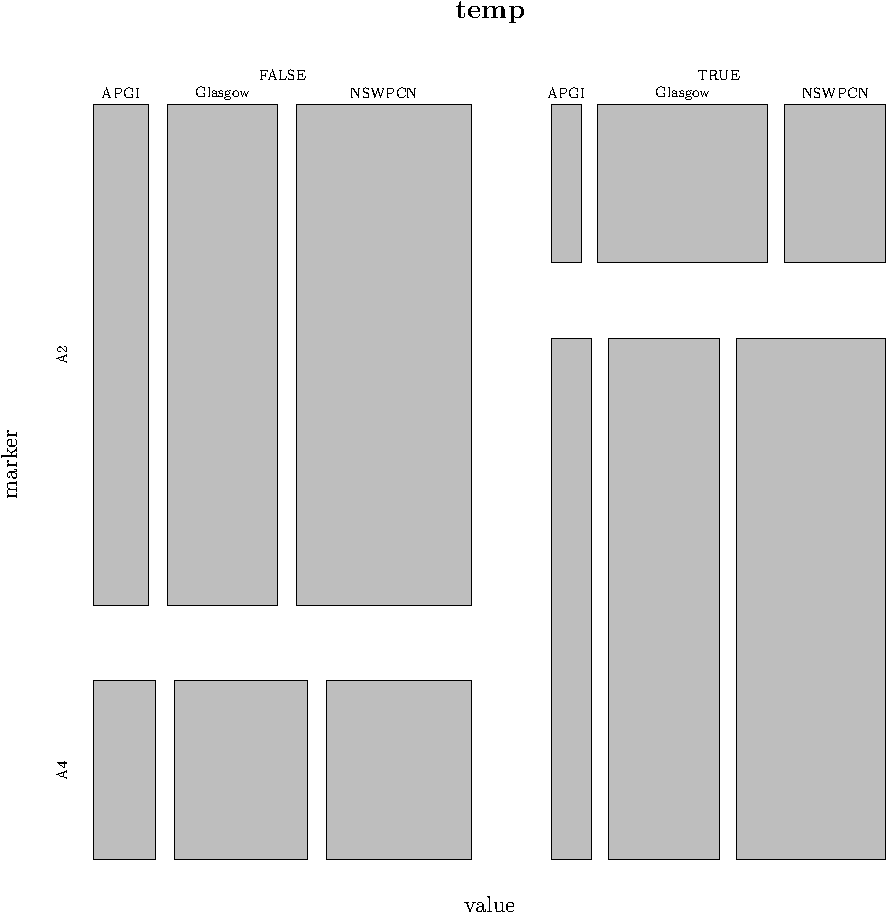
\includegraphics[width=\maxwidth]{figure/07-data-summaries-1} 

}


\begin{kframe}\begin{alltt}
\hlkwd{plot}\hlstd{(}\hlkwd{as.table}\hlstd{(temp[,}\hlnum{1}\hlstd{,]))}
\end{alltt}
\end{kframe}

{\centering 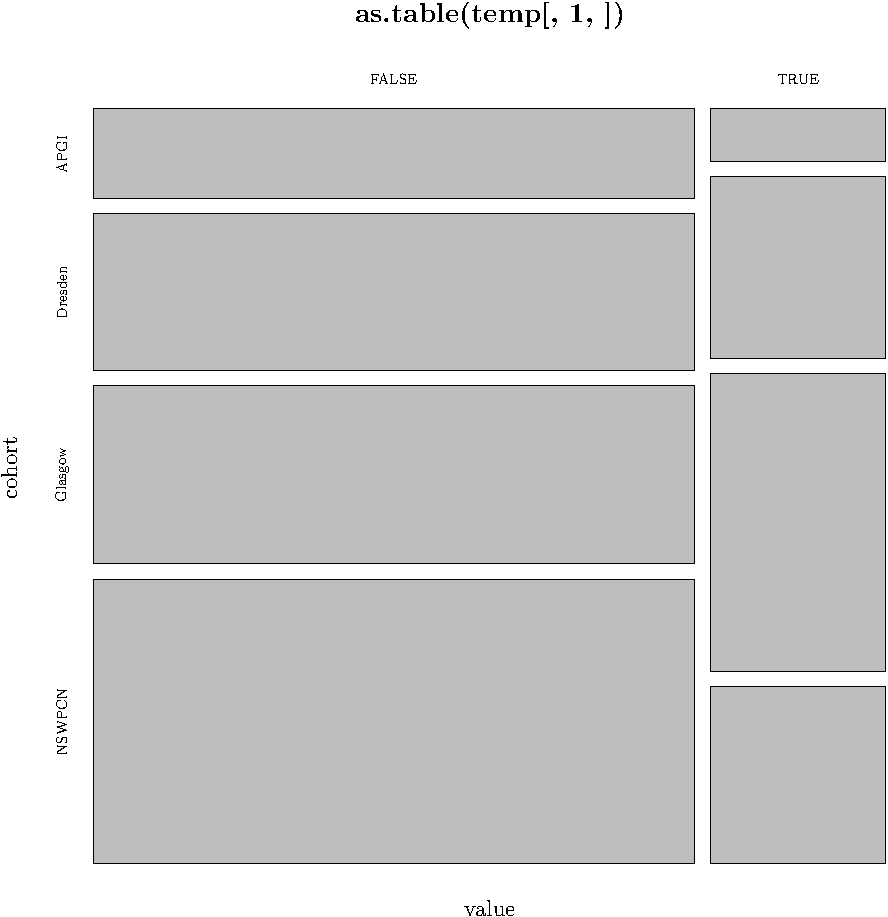
\includegraphics[width=\maxwidth]{figure/07-data-summaries-2} 

}


\begin{kframe}\begin{alltt}
\hlkwd{plot}\hlstd{(}\hlkwd{as.table}\hlstd{(temp[,}\hlnum{2}\hlstd{,]))}
\end{alltt}
\end{kframe}

{\centering 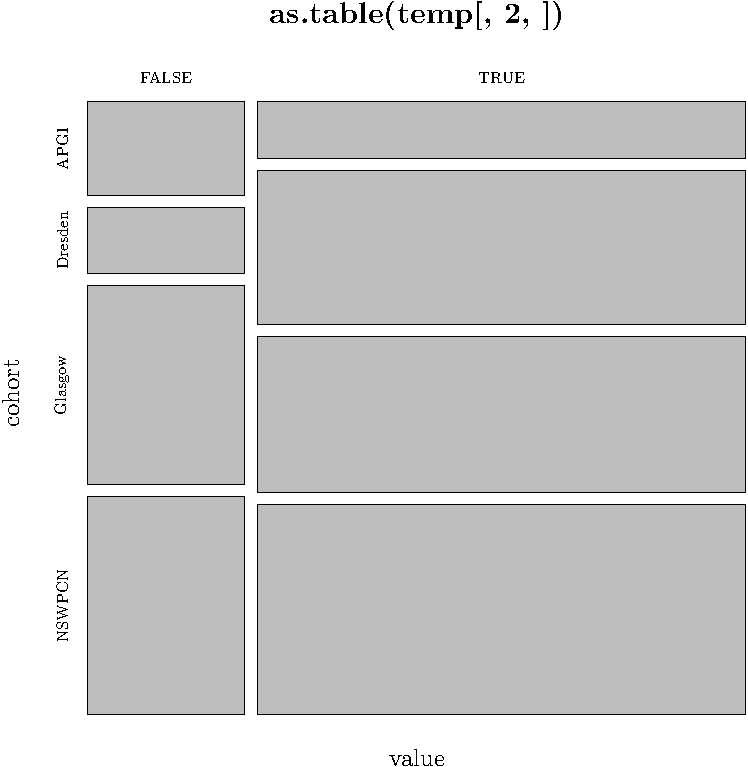
\includegraphics[width=\maxwidth]{figure/07-data-summaries-3} 

}



\end{knitrout}

\begin{knitrout}
\definecolor{shadecolor}{rgb}{0.969, 0.969, 0.969}\color{fgcolor}\begin{kframe}
\begin{alltt}
\hlstd{temp.time} \hlkwb{=} \hlkwd{c}\hlstd{(data.nswpcn}\hlopt{$}\hlstd{Time, data.glasgow}\hlopt{$}\hlstd{Time, data.apgi}\hlopt{$}\hlstd{Time)} \hlopt{/} \hlnum{365.25}
\hlstd{temp.dsd} \hlkwb{=} \hlkwd{c}\hlstd{(data.nswpcn}\hlopt{$}\hlstd{DSD, data.glasgow}\hlopt{$}\hlstd{DSD, data.apgi}\hlopt{$}\hlstd{DSD)}
\hlstd{temp.cohort} \hlkwb{=} \hlkwd{factor}\hlstd{(}\hlkwd{rep}\hlstd{(}\hlkwd{c}\hlstd{(}\hlstr{"NSWPCN"}\hlstd{,} \hlstr{"Glasgow"}\hlstd{,} \hlstr{"APGI"}\hlstd{),} \hlkwd{c}\hlstd{(}\hlkwd{nrow}\hlstd{(data.nswpcn),} \hlkwd{nrow}\hlstd{(data.glasgow),} \hlkwd{nrow}\hlstd{(data.apgi))))}
\hlstd{temp.survfit} \hlkwb{=} \hlkwd{survfit}\hlstd{(}\hlkwd{Surv}\hlstd{(temp.time, temp.dsd)} \hlopt{~} \hlstd{temp.cohort)}
\hlkwd{plot}\hlstd{(temp.survfit,} \hlkwc{col} \hlstd{= pal[}\hlnum{1}\hlopt{:}\hlnum{3}\hlstd{],} \hlkwc{xlim} \hlstd{=} \hlkwd{c}\hlstd{(}\hlnum{0}\hlstd{,} \hlnum{5}\hlstd{),} \hlkwc{lwd} \hlstd{=} \hlnum{2}\hlstd{,} \hlkwc{main} \hlstd{=} \hlstr{"Cohort marginal survival"}\hlstd{,} \hlkwc{xlab} \hlstd{=} \hlstr{"Time from diagnosis (years)"}\hlstd{,} \hlkwc{ylab} \hlstd{=} \hlstr{"Fraction alive"}\hlstd{)}
\hlkwd{legend}\hlstd{(}\hlstr{"topright"}\hlstd{,} \hlkwc{legend} \hlstd{=} \hlkwd{c}\hlstd{(}\hlstr{"APGI"}\hlstd{,} \hlstr{"Glasgow"}\hlstd{,} \hlstr{"NSWPCN"}\hlstd{),} \hlkwc{col} \hlstd{= pal[}\hlnum{1}\hlopt{:}\hlnum{3}\hlstd{],} \hlkwc{inset} \hlstd{=} \hlnum{0.05}\hlstd{,} \hlkwc{lwd} \hlstd{=} \hlnum{2}\hlstd{)}
\end{alltt}
\end{kframe}

{\centering 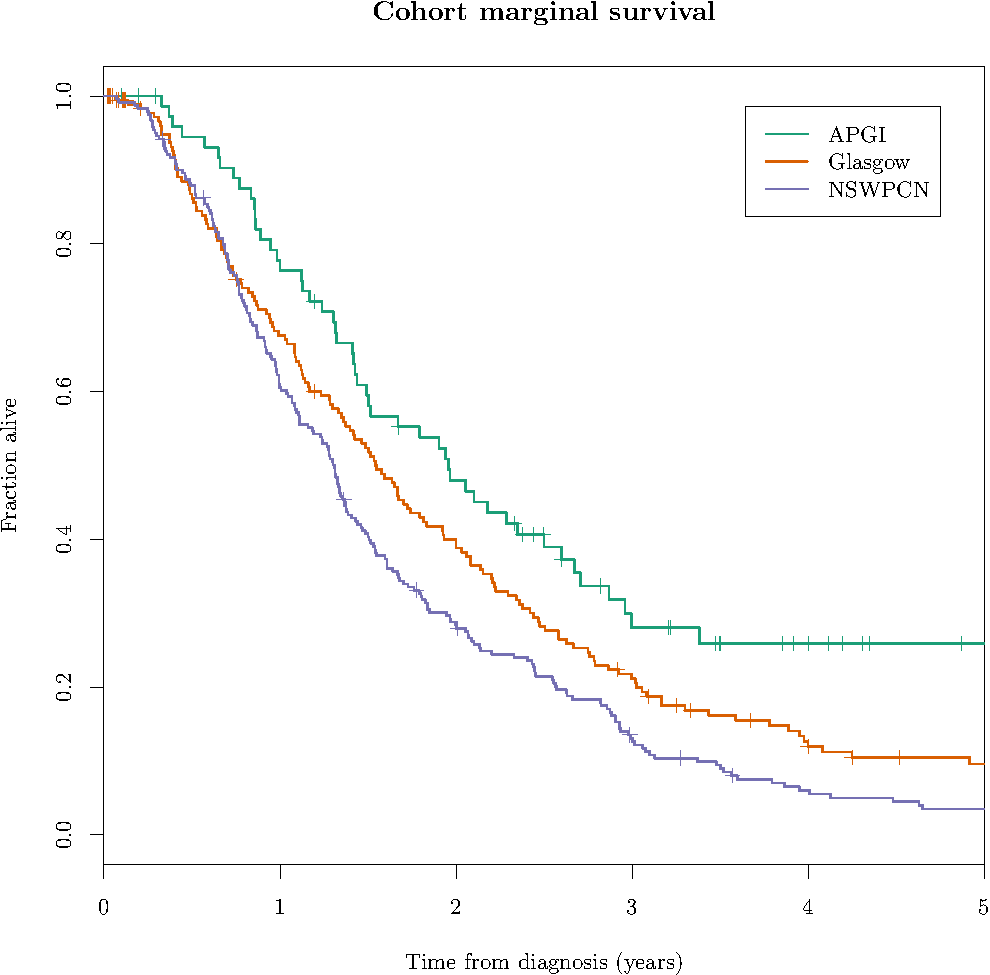
\includegraphics[width=\maxwidth]{figure/07-cohort-surv-comparison-1} 

}



\end{knitrout}


\section{Score calculation}
\begin{knitrout}
\definecolor{shadecolor}{rgb}{0.969, 0.969, 0.969}\color{fgcolor}\begin{kframe}
\begin{alltt}
\hlstd{temp} \hlkwb{=} \hlkwd{applyNomogram}\hlstd{(fit.mskcc, data.glasgow)}
\end{alltt}


{\ttfamily\noindent\color{warningcolor}{\#\# Warning in FUN(c("{}History.Diagnosis.AgeAt"{}, "{}Patient.Sex"{}, "{}Portal.Vein"{}, : Marginalizing missing variable: Portal.Vein}}

{\ttfamily\noindent\color{warningcolor}{\#\# Warning in FUN(c("{}History.Diagnosis.AgeAt"{}, "{}Patient.Sex"{}, "{}Portal.Vein"{}, : Marginalizing missing variable: Splenectomy}}

{\ttfamily\noindent\color{warningcolor}{\#\# Warning in FUN(c("{}History.Diagnosis.AgeAt"{}, "{}Patient.Sex"{}, "{}Portal.Vein"{}, : Marginalizing missing variable: Posterior.Margin}}

{\ttfamily\noindent\color{warningcolor}{\#\# Warning in FUN(c("{}History.Diagnosis.AgeAt"{}, "{}Patient.Sex"{}, "{}Portal.Vein"{}, : Marginalizing missing variable: Back.pain}}

{\ttfamily\noindent\color{warningcolor}{\#\# Warning in FUN(c("{}History.Diagnosis.AgeAt"{}, "{}Patient.Sex"{}, "{}Portal.Vein"{}, : Marginalizing missing variable: Weight.loss}}\begin{alltt}
\hlstd{mskcc_post.linpred.glasgow} \hlkwb{=} \hlstd{temp[,}\hlnum{1}\hlstd{]}
\hlstd{mskcc_post.12mo.glasgow} \hlkwb{=} \hlstd{temp[,}\hlnum{2}\hlstd{]}
\hlstd{mskcc_post.24mo.glasgow} \hlkwb{=} \hlstd{temp[,}\hlnum{3}\hlstd{]}
\hlstd{mskcc_post.36mo.glasgow} \hlkwb{=} \hlstd{temp[,}\hlnum{4}\hlstd{]}
\hlstd{temp} \hlkwb{=} \hlkwd{applyNomogram}\hlstd{(fit.mskcc, data.glasgow[,}\hlkwd{c}\hlstd{(}\hlstr{"History.Diagnosis.AgeAt"}\hlstd{,} \hlstr{"Patient.Sex"}\hlstd{,} \hlstr{"Path.LocationBody"}\hlstd{,} \hlstr{"Stage.pT.Simplified"}\hlstd{,} \hlstr{"Path.Size"}\hlstd{)])}
\end{alltt}


{\ttfamily\noindent\color{warningcolor}{\#\# Warning in FUN(c("{}History.Diagnosis.AgeAt"{}, "{}Patient.Sex"{}, "{}Portal.Vein"{}, : Marginalizing missing variable: Portal.Vein}}

{\ttfamily\noindent\color{warningcolor}{\#\# Warning in FUN(c("{}History.Diagnosis.AgeAt"{}, "{}Patient.Sex"{}, "{}Portal.Vein"{}, : Marginalizing missing variable: Splenectomy}}

{\ttfamily\noindent\color{warningcolor}{\#\# Warning in FUN(c("{}History.Diagnosis.AgeAt"{}, "{}Patient.Sex"{}, "{}Portal.Vein"{}, : Marginalizing missing variable: Treat.MarginPositive}}

{\ttfamily\noindent\color{warningcolor}{\#\# Warning in FUN(c("{}History.Diagnosis.AgeAt"{}, "{}Patient.Sex"{}, "{}Portal.Vein"{}, : Marginalizing missing variable: Path.Differentiation}}

{\ttfamily\noindent\color{warningcolor}{\#\# Warning in FUN(c("{}History.Diagnosis.AgeAt"{}, "{}Patient.Sex"{}, "{}Portal.Vein"{}, : Marginalizing missing variable: Posterior.Margin}}

{\ttfamily\noindent\color{warningcolor}{\#\# Warning in FUN(c("{}History.Diagnosis.AgeAt"{}, "{}Patient.Sex"{}, "{}Portal.Vein"{}, : Marginalizing missing variable: Path.LN.Involved}}

{\ttfamily\noindent\color{warningcolor}{\#\# Warning in FUN(c("{}History.Diagnosis.AgeAt"{}, "{}Patient.Sex"{}, "{}Portal.Vein"{}, : Marginalizing missing variable: Path.LN.Negative}}

{\ttfamily\noindent\color{warningcolor}{\#\# Warning in FUN(c("{}History.Diagnosis.AgeAt"{}, "{}Patient.Sex"{}, "{}Portal.Vein"{}, : Marginalizing missing variable: Back.pain}}

{\ttfamily\noindent\color{warningcolor}{\#\# Warning in FUN(c("{}History.Diagnosis.AgeAt"{}, "{}Patient.Sex"{}, "{}Portal.Vein"{}, : Marginalizing missing variable: Weight.loss}}\begin{alltt}
\hlstd{mskcc_pre.linpred.glasgow} \hlkwb{=} \hlstd{temp[,}\hlnum{1}\hlstd{]}
\hlstd{mskcc_pre.12mo.glasgow} \hlkwb{=} \hlstd{temp[,}\hlnum{2}\hlstd{]}
\hlstd{mskcc_pre.24mo.glasgow} \hlkwb{=} \hlstd{temp[,}\hlnum{3}\hlstd{]}
\hlstd{mskcc_pre.36mo.glasgow} \hlkwb{=} \hlstd{temp[,}\hlnum{4}\hlstd{]}

\hlstd{temp} \hlkwb{=} \hlkwd{applyNomogram}\hlstd{(fit.mskcc, data.apgi)}
\end{alltt}


{\ttfamily\noindent\color{warningcolor}{\#\# Warning in FUN(c("{}History.Diagnosis.AgeAt"{}, "{}Patient.Sex"{}, "{}Portal.Vein"{}, : Marginalizing missing variable: Portal.Vein}}

{\ttfamily\noindent\color{warningcolor}{\#\# Warning in FUN(c("{}History.Diagnosis.AgeAt"{}, "{}Patient.Sex"{}, "{}Portal.Vein"{}, : Marginalizing missing variable: Splenectomy}}

{\ttfamily\noindent\color{warningcolor}{\#\# Warning in FUN(c("{}History.Diagnosis.AgeAt"{}, "{}Patient.Sex"{}, "{}Portal.Vein"{}, : Marginalizing missing variable: Posterior.Margin}}

{\ttfamily\noindent\color{warningcolor}{\#\# Warning in FUN(c("{}History.Diagnosis.AgeAt"{}, "{}Patient.Sex"{}, "{}Portal.Vein"{}, : Marginalizing missing variable: Back.pain}}

{\ttfamily\noindent\color{warningcolor}{\#\# Warning in FUN(c("{}History.Diagnosis.AgeAt"{}, "{}Patient.Sex"{}, "{}Portal.Vein"{}, : Marginalizing missing variable: Weight.loss}}\begin{alltt}
\hlstd{mskcc_post.linpred.apgi} \hlkwb{=} \hlstd{temp[,}\hlnum{1}\hlstd{]}
\hlstd{mskcc_post.12mo.apgi} \hlkwb{=} \hlstd{temp[,}\hlnum{2}\hlstd{]}
\hlstd{mskcc_post.24mo.apgi} \hlkwb{=} \hlstd{temp[,}\hlnum{3}\hlstd{]}
\hlstd{mskcc_post.36mo.apgi} \hlkwb{=} \hlstd{temp[,}\hlnum{4}\hlstd{]}
\hlstd{temp} \hlkwb{=} \hlkwd{applyNomogram}\hlstd{(fit.mskcc, data.apgi[,}\hlkwd{c}\hlstd{(}\hlstr{"History.Diagnosis.AgeAt"}\hlstd{,} \hlstr{"Patient.Sex"}\hlstd{,} \hlstr{"Path.LocationBody"}\hlstd{,} \hlstr{"Stage.pT.Simplified"}\hlstd{,} \hlstr{"Path.Size"}\hlstd{)])}
\end{alltt}


{\ttfamily\noindent\color{warningcolor}{\#\# Warning in FUN(c("{}History.Diagnosis.AgeAt"{}, "{}Patient.Sex"{}, "{}Portal.Vein"{}, : Marginalizing missing variable: Portal.Vein}}

{\ttfamily\noindent\color{warningcolor}{\#\# Warning in FUN(c("{}History.Diagnosis.AgeAt"{}, "{}Patient.Sex"{}, "{}Portal.Vein"{}, : Marginalizing missing variable: Splenectomy}}

{\ttfamily\noindent\color{warningcolor}{\#\# Warning in FUN(c("{}History.Diagnosis.AgeAt"{}, "{}Patient.Sex"{}, "{}Portal.Vein"{}, : Marginalizing missing variable: Treat.MarginPositive}}

{\ttfamily\noindent\color{warningcolor}{\#\# Warning in FUN(c("{}History.Diagnosis.AgeAt"{}, "{}Patient.Sex"{}, "{}Portal.Vein"{}, : Marginalizing missing variable: Path.Differentiation}}

{\ttfamily\noindent\color{warningcolor}{\#\# Warning in FUN(c("{}History.Diagnosis.AgeAt"{}, "{}Patient.Sex"{}, "{}Portal.Vein"{}, : Marginalizing missing variable: Posterior.Margin}}

{\ttfamily\noindent\color{warningcolor}{\#\# Warning in FUN(c("{}History.Diagnosis.AgeAt"{}, "{}Patient.Sex"{}, "{}Portal.Vein"{}, : Marginalizing missing variable: Path.LN.Involved}}

{\ttfamily\noindent\color{warningcolor}{\#\# Warning in FUN(c("{}History.Diagnosis.AgeAt"{}, "{}Patient.Sex"{}, "{}Portal.Vein"{}, : Marginalizing missing variable: Path.LN.Negative}}

{\ttfamily\noindent\color{warningcolor}{\#\# Warning in FUN(c("{}History.Diagnosis.AgeAt"{}, "{}Patient.Sex"{}, "{}Portal.Vein"{}, : Marginalizing missing variable: Back.pain}}

{\ttfamily\noindent\color{warningcolor}{\#\# Warning in FUN(c("{}History.Diagnosis.AgeAt"{}, "{}Patient.Sex"{}, "{}Portal.Vein"{}, : Marginalizing missing variable: Weight.loss}}\begin{alltt}
\hlstd{mskcc_pre.linpred.apgi} \hlkwb{=} \hlstd{temp[,}\hlnum{1}\hlstd{]}
\hlstd{mskcc_pre.12mo.apgi} \hlkwb{=} \hlstd{temp[,}\hlnum{2}\hlstd{]}
\hlstd{mskcc_pre.24mo.apgi} \hlkwb{=} \hlstd{temp[,}\hlnum{3}\hlstd{]}
\hlstd{mskcc_pre.36mo.apgi} \hlkwb{=} \hlstd{temp[,}\hlnum{4}\hlstd{]}
\end{alltt}
\end{kframe}
\end{knitrout}

Get approximate linear predictors from the GG model, by just calculating the location term.
\begin{knitrout}
\definecolor{shadecolor}{rgb}{0.969, 0.969, 0.969}\color{fgcolor}\begin{kframe}
\begin{alltt}
\hlstd{val.prob.times} \hlkwb{=} \hlkwd{seq}\hlstd{(}\hlnum{0}\hlstd{,} \hlkwd{max}\hlstd{(}\hlkwd{c}\hlstd{(data.glasgow}\hlopt{$}\hlstd{Time, data.apgi}\hlopt{$}\hlstd{Time)),} \hlnum{1}\hlstd{)}
\end{alltt}
\end{kframe}
\end{knitrout}

\begin{knitrout}
\definecolor{shadecolor}{rgb}{0.969, 0.969, 0.969}\color{fgcolor}\begin{kframe}
\begin{alltt}
\hlstd{gg.path.glasgow} \hlkwb{=} \hlkwd{summary}\hlstd{(fit.gg,} \hlkwc{newdata} \hlstd{= data.glasgow,} \hlkwc{ci} \hlstd{=} \hlnum{FALSE}\hlstd{)}
\hlstd{temp.coefs} \hlkwb{=} \hlkwd{coef}\hlstd{(fit.gg)}
\hlstd{gg.linpred.glasgow} \hlkwb{=} \hlkwd{sapply}\hlstd{(}\hlnum{1}\hlopt{:}\hlkwd{length}\hlstd{(temp.coefs),} \hlkwa{function}\hlstd{(}\hlkwc{coef_i}\hlstd{) \{}
        \hlcom{# if (names(temp.coefs)[coef_i] == "SexMTRUE") \{}
 \hlcom{#        rep(0, nrow(data.val)) }
        \hlcom{# \} else }
        \hlkwa{if} \hlstd{(}\hlkwd{names}\hlstd{(temp.coefs)[coef_i]} \hlopt \hlkwd{colnames}\hlstd{(data.glasgow)) \{}
                \hlstd{temp.coefs[coef_i]} \hlopt{*} \hlstd{data.glasgow[,}\hlkwd{names}\hlstd{(temp.coefs)[coef_i]]}
        \hlstd{\}} \hlkwa{else if} \hlstd{(}\hlkwd{gsub}\hlstd{(}\hlstr{"TRUE$"}\hlstd{,} \hlstr{""}\hlstd{,} \hlkwd{names}\hlstd{(temp.coefs)[coef_i])} \hlopt \hlkwd{colnames}\hlstd{(data.glasgow)) \{}
                \hlstd{temp.coefs[coef_i]} \hlopt{*} \hlstd{data.glasgow[,}\hlkwd{gsub}\hlstd{(}\hlstr{"TRUE$"}\hlstd{,} \hlstr{""}\hlstd{,} \hlkwd{names}\hlstd{(temp.coefs)[coef_i])]}
        \hlstd{\}} \hlkwa{else} \hlstd{\{}
                \hlkwd{rep}\hlstd{(}\hlnum{0}\hlstd{,} \hlkwd{nrow}\hlstd{(data.glasgow))}
        \hlstd{\} \})}
\hlstd{gg.linpred.glasgow} \hlkwb{=} \hlopt{-}\hlkwd{rowSums}\hlstd{(gg.linpred.glasgow)}       \hlcom{# Negate to bring into concordance with the direction of Cox coefficients (ie higher is now worse)}
\hlstd{temp} \hlkwb{=} \hlkwd{summary}\hlstd{(fit.gg,} \hlkwc{newdata} \hlstd{= data.glasgow,} \hlkwc{ci} \hlstd{=} \hlnum{FALSE}\hlstd{)}
\hlstd{gg.prob.glasgow} \hlkwb{=} \hlkwd{sapply}\hlstd{(temp,} \hlkwa{function}\hlstd{(}\hlkwc{x}\hlstd{)} \hlkwd{approx}\hlstd{(x[,}\hlnum{1}\hlstd{], x[,}\hlnum{2}\hlstd{],} \hlkwc{xout} \hlstd{= val.prob.times,} \hlkwc{yleft} \hlstd{=} \hlnum{1}\hlstd{,} \hlkwc{yright} \hlstd{=} \hlnum{0}\hlstd{,} \hlkwc{rule} \hlstd{=} \hlnum{2}\hlstd{)}\hlopt{$}\hlstd{y)}
\hlkwd{colnames}\hlstd{(gg.prob.glasgow)} \hlkwb{=} \hlkwd{rownames}\hlstd{(data.glasgow)}
\end{alltt}
\end{kframe}
\end{knitrout}

\begin{knitrout}
\definecolor{shadecolor}{rgb}{0.969, 0.969, 0.969}\color{fgcolor}\begin{kframe}
\begin{alltt}
\hlstd{gg.path.apgi} \hlkwb{=} \hlkwd{summary}\hlstd{(fit.gg,} \hlkwc{newdata} \hlstd{= data.apgi,} \hlkwc{ci} \hlstd{=} \hlnum{FALSE}\hlstd{)}
\hlstd{temp.coefs} \hlkwb{=} \hlkwd{coef}\hlstd{(fit.gg)}
\hlstd{gg.linpred.apgi} \hlkwb{=} \hlkwd{sapply}\hlstd{(}\hlnum{1}\hlopt{:}\hlkwd{length}\hlstd{(temp.coefs),} \hlkwa{function}\hlstd{(}\hlkwc{coef_i}\hlstd{) \{}
        \hlcom{# if (names(temp.coefs)[coef_i] == "SexMTRUE") \{}
 \hlcom{#        rep(0, nrow(data.val)) }
        \hlcom{# \} else }
        \hlkwa{if} \hlstd{(}\hlkwd{names}\hlstd{(temp.coefs)[coef_i]} \hlopt \hlkwd{colnames}\hlstd{(data.apgi)) \{}
                \hlstd{temp.coefs[coef_i]} \hlopt{*} \hlstd{data.apgi[,}\hlkwd{names}\hlstd{(temp.coefs)[coef_i]]}
        \hlstd{\}} \hlkwa{else if} \hlstd{(}\hlkwd{gsub}\hlstd{(}\hlstr{"TRUE$"}\hlstd{,} \hlstr{""}\hlstd{,} \hlkwd{names}\hlstd{(temp.coefs)[coef_i])} \hlopt \hlkwd{colnames}\hlstd{(data.apgi)) \{}
                \hlstd{temp.coefs[coef_i]} \hlopt{*} \hlstd{data.apgi[,}\hlkwd{gsub}\hlstd{(}\hlstr{"TRUE$"}\hlstd{,} \hlstr{""}\hlstd{,} \hlkwd{names}\hlstd{(temp.coefs)[coef_i])]}
        \hlstd{\}} \hlkwa{else} \hlstd{\{}
                \hlkwd{rep}\hlstd{(}\hlnum{0}\hlstd{,} \hlkwd{nrow}\hlstd{(data.apgi))}
        \hlstd{\} \})}
\hlstd{gg.linpred.apgi} \hlkwb{=} \hlopt{-}\hlkwd{rowSums}\hlstd{(gg.linpred.apgi)}     \hlcom{# Negate to bring into concordance with the direction of Cox coefficients (ie higher is now worse)}
\hlstd{temp} \hlkwb{=} \hlkwd{summary}\hlstd{(fit.gg,} \hlkwc{newdata} \hlstd{= data.apgi,} \hlkwc{ci} \hlstd{=} \hlnum{FALSE}\hlstd{)}
\hlstd{gg.prob.apgi} \hlkwb{=} \hlkwd{sapply}\hlstd{(temp,} \hlkwa{function}\hlstd{(}\hlkwc{x}\hlstd{)} \hlkwd{approx}\hlstd{(x[,}\hlnum{1}\hlstd{], x[,}\hlnum{2}\hlstd{],} \hlkwc{xout} \hlstd{= val.prob.times,} \hlkwc{yleft} \hlstd{=} \hlnum{1}\hlstd{,} \hlkwc{yright} \hlstd{=} \hlnum{0}\hlstd{,} \hlkwc{rule} \hlstd{=} \hlnum{2}\hlstd{)}\hlopt{$}\hlstd{y)}
\hlkwd{colnames}\hlstd{(gg.prob.apgi)} \hlkwb{=} \hlkwd{rownames}\hlstd{(data.apgi)}
\end{alltt}
\end{kframe}
\end{knitrout}

\begin{knitrout}
\definecolor{shadecolor}{rgb}{0.969, 0.969, 0.969}\color{fgcolor}\begin{kframe}
\begin{alltt}
\hlstd{gg.linpred.nswpcn} \hlkwb{=} \hlkwd{sapply}\hlstd{(}\hlnum{1}\hlopt{:}\hlkwd{length}\hlstd{(temp.coefs),} \hlkwa{function}\hlstd{(}\hlkwc{coef_i}\hlstd{) \{}
        \hlcom{# if (names(temp.coefs)[coef_i] == "SexMTRUE") \{}
 \hlcom{#        rep(0, nrow(data.val)) }
        \hlcom{# \} else }
        \hlkwa{if} \hlstd{(}\hlkwd{names}\hlstd{(temp.coefs)[coef_i]} \hlopt \hlkwd{colnames}\hlstd{(data.glasgow)) \{}
                \hlstd{temp.coefs[coef_i]} \hlopt{*} \hlstd{data.nswpcn[,}\hlkwd{names}\hlstd{(temp.coefs)[coef_i]]}
        \hlstd{\}} \hlkwa{else if} \hlstd{(}\hlkwd{gsub}\hlstd{(}\hlstr{"TRUE$"}\hlstd{,} \hlstr{""}\hlstd{,} \hlkwd{names}\hlstd{(temp.coefs)[coef_i])} \hlopt \hlkwd{colnames}\hlstd{(data.nswpcn)) \{}
                \hlstd{temp.coefs[coef_i]} \hlopt{*} \hlstd{data.nswpcn[,}\hlkwd{gsub}\hlstd{(}\hlstr{"TRUE$"}\hlstd{,} \hlstr{""}\hlstd{,} \hlkwd{names}\hlstd{(temp.coefs)[coef_i])]}
        \hlstd{\}} \hlkwa{else} \hlstd{\{}
                \hlkwd{rep}\hlstd{(}\hlnum{0}\hlstd{,} \hlkwd{nrow}\hlstd{(data.nswpcn))}
        \hlstd{\} \})}
\hlstd{gg.linpred.nswpcn} \hlkwb{=} \hlopt{-}\hlkwd{rowSums}\hlstd{(gg.linpred.nswpcn)}         \hlcom{# Negate to bring into concordance with the direction of Cox coefficients (ie higher is now worse)}
\hlstd{temp} \hlkwb{=} \hlkwd{summary}\hlstd{(fit.gg,} \hlkwc{newdata} \hlstd{= data.nswpcn,} \hlkwc{ci} \hlstd{=} \hlnum{FALSE}\hlstd{)}
\hlstd{gg.prob.nswpcn} \hlkwb{=} \hlkwd{sapply}\hlstd{(temp,} \hlkwa{function}\hlstd{(}\hlkwc{x}\hlstd{)} \hlkwd{approx}\hlstd{(x[,}\hlnum{1}\hlstd{], x[,}\hlnum{2}\hlstd{],} \hlkwc{xout} \hlstd{= val.prob.times,} \hlkwc{yleft} \hlstd{=} \hlnum{1}\hlstd{,} \hlkwc{yright} \hlstd{=} \hlnum{0}\hlstd{,} \hlkwc{rule} \hlstd{=} \hlnum{2}\hlstd{)}\hlopt{$}\hlstd{y)}
\hlkwd{colnames}\hlstd{(gg.prob.nswpcn)} \hlkwb{=} \hlkwd{rownames}\hlstd{(data.nswpcn)}
\end{alltt}
\end{kframe}
\end{knitrout}

\section{Validation}
\subsection{Altman diagnostic 1: score histograms}
\begin{knitrout}
\definecolor{shadecolor}{rgb}{0.969, 0.969, 0.969}\color{fgcolor}\begin{kframe}
\begin{alltt}
\hlkwd{par}\hlstd{(}\hlkwc{mfrow} \hlstd{=} \hlkwd{c}\hlstd{(}\hlnum{3}\hlstd{,} \hlnum{1}\hlstd{))}
\hlkwd{hist}\hlstd{(gg.linpred.nswpcn,} \hlkwc{main} \hlstd{=} \hlstr{"NSWPCN GG scores"}\hlstd{,} \hlkwc{xlim} \hlstd{=} \hlkwd{range}\hlstd{(}\hlkwd{c}\hlstd{(gg.linpred.nswpcn, gg.linpred.glasgow, gg.linpred.apgi)),} \hlkwc{breaks} \hlstd{=} \hlnum{20}\hlstd{,} \hlkwc{col} \hlstd{=} \hlstr{"grey"}\hlstd{)}
\hlkwd{abline}\hlstd{(}\hlkwc{v} \hlstd{=} \hlkwd{quantile}\hlstd{(gg.linpred.nswpcn,} \hlkwc{probs} \hlstd{=} \hlkwd{c}\hlstd{(}\hlnum{0.25}\hlstd{,} \hlnum{0.5}\hlstd{,} \hlnum{0.75}\hlstd{)),} \hlkwc{col} \hlstd{=} \hlstr{"red"}\hlstd{)}
\hlkwd{hist}\hlstd{(gg.linpred.glasgow,} \hlkwc{main} \hlstd{=} \hlstr{"Glasgow GG scores"}\hlstd{,} \hlkwc{xlim} \hlstd{=} \hlkwd{range}\hlstd{(}\hlkwd{c}\hlstd{(gg.linpred.nswpcn, gg.linpred.glasgow, gg.linpred.apgi)),} \hlkwc{breaks} \hlstd{=} \hlnum{20}\hlstd{,} \hlkwc{col} \hlstd{=} \hlstr{"grey"}\hlstd{)}
\hlkwd{abline}\hlstd{(}\hlkwc{v} \hlstd{=} \hlkwd{quantile}\hlstd{(gg.linpred.glasgow,} \hlkwc{probs} \hlstd{=} \hlkwd{c}\hlstd{(}\hlnum{0.25}\hlstd{,} \hlnum{0.5}\hlstd{,} \hlnum{0.75}\hlstd{)),} \hlkwc{col} \hlstd{=} \hlstr{"red"}\hlstd{)}
\hlkwd{hist}\hlstd{(gg.linpred.apgi,} \hlkwc{main} \hlstd{=} \hlstr{"APGI GG scores"}\hlstd{,} \hlkwc{xlim} \hlstd{=} \hlkwd{range}\hlstd{(}\hlkwd{c}\hlstd{(gg.linpred.nswpcn, gg.linpred.glasgow, gg.linpred.apgi)),} \hlkwc{breaks} \hlstd{=} \hlnum{20}\hlstd{,} \hlkwc{col} \hlstd{=} \hlstr{"grey"}\hlstd{)}
\hlkwd{abline}\hlstd{(}\hlkwc{v} \hlstd{=} \hlkwd{quantile}\hlstd{(gg.linpred.apgi,} \hlkwc{probs} \hlstd{=} \hlkwd{c}\hlstd{(}\hlnum{0.25}\hlstd{,} \hlnum{0.5}\hlstd{,} \hlnum{0.75}\hlstd{)),} \hlkwc{col} \hlstd{=} \hlstr{"red"}\hlstd{)}
\end{alltt}
\end{kframe}

{\centering 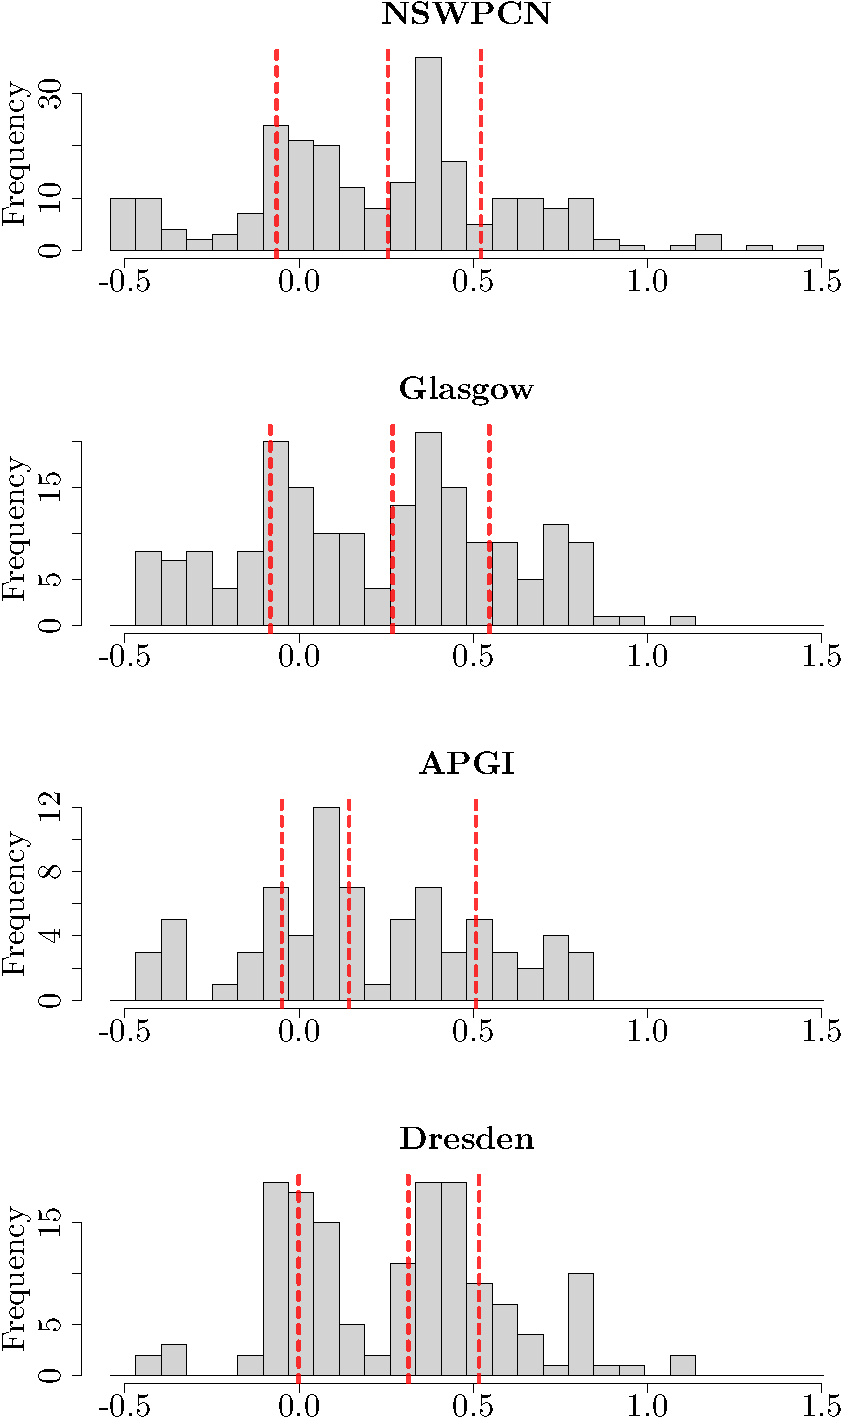
\includegraphics[width=\maxwidth]{figure/07-score-hists-1} 

}


\begin{kframe}\begin{alltt}
\hlkwd{par}\hlstd{(}\hlkwc{mfrow} \hlstd{=} \hlkwd{c}\hlstd{(}\hlnum{1}\hlstd{,} \hlnum{1}\hlstd{))}
\end{alltt}
\end{kframe}
\end{knitrout}

\subsection{Altman method 1 (D,F)}
\begin{knitrout}
\definecolor{shadecolor}{rgb}{0.969, 0.969, 0.969}\color{fgcolor}\begin{kframe}
\begin{alltt}
\hlkwd{summary}\hlstd{(}\hlkwd{coxph}\hlstd{(}\hlkwd{Surv}\hlstd{(Time, DSD)} \hlopt{~} \hlstd{mskcc_post.linpred.glasgow, data.glasgow))}
\end{alltt}
\begin{verbatim}
## Call:
## coxph(formula = Surv(Time, DSD) ~ mskcc_post.linpred.glasgow, 
##     data = data.glasgow)
## 
##   n= 189, number of events= 161 
## 
##                               coef exp(coef) se(coef)    z Pr(>|z|)
## mskcc_post.linpred.glasgow 0.01682   1.01696  0.00428 3.93  8.4e-05
## 
##                            exp(coef) exp(-coef) lower .95 upper .95
## mskcc_post.linpred.glasgow      1.02      0.983      1.01      1.03
## 
## Concordance= 0.584  (se = 0.026 )
## Rsquare= 0.081   (max possible= 0.999 )
## Likelihood ratio test= 15.9  on 1 df,   p=6.79e-05
## Wald test            = 15.5  on 1 df,   p=8.43e-05
## Score (logrank) test = 15.7  on 1 df,   p=7.56e-05
\end{verbatim}
\begin{alltt}
\hlkwd{summary}\hlstd{(}\hlkwd{coxph}\hlstd{(}\hlkwd{Surv}\hlstd{(Time, DSD)} \hlopt{~} \hlstd{mskcc_pre.linpred.glasgow, data.glasgow))}
\end{alltt}
\begin{verbatim}
## Call:
## coxph(formula = Surv(Time, DSD) ~ mskcc_pre.linpred.glasgow, 
##     data = data.glasgow)
## 
##   n= 189, number of events= 161 
## 
##                             coef exp(coef) se(coef)    z Pr(>|z|)
## mskcc_pre.linpred.glasgow 0.0118    1.0118   0.0105 1.12     0.26
## 
##                           exp(coef) exp(-coef) lower .95 upper .95
## mskcc_pre.linpred.glasgow      1.01      0.988     0.991      1.03
## 
## Concordance= 0.585  (se = 0.026 )
## Rsquare= 0.006   (max possible= 0.999 )
## Likelihood ratio test= 1.15  on 1 df,   p=0.284
## Wald test            = 1.25  on 1 df,   p=0.263
## Score (logrank) test = 1.25  on 1 df,   p=0.264
\end{verbatim}
\begin{alltt}
\hlkwd{summary}\hlstd{(}\hlkwd{coxph}\hlstd{(}\hlkwd{Surv}\hlstd{(Time, DSD)} \hlopt{~} \hlstd{mskcc_post.linpred.apgi, data.apgi))}
\end{alltt}
\begin{verbatim}
## Call:
## coxph(formula = Surv(Time, DSD) ~ mskcc_post.linpred.apgi, data = data.apgi)
## 
##   n= 75, number of events= 51 
## 
##                            coef exp(coef) se(coef)   z Pr(>|z|)
## mskcc_post.linpred.apgi 0.01626   1.01639  0.00452 3.6  0.00032
## 
##                         exp(coef) exp(-coef) lower .95 upper .95
## mskcc_post.linpred.apgi      1.02      0.984      1.01      1.03
## 
## Concordance= 0.701  (se = 0.044 )
## Rsquare= 0.14   (max possible= 0.993 )
## Likelihood ratio test= 11.3  on 1 df,   p=0.000754
## Wald test            = 12.9  on 1 df,   p=0.000319
## Score (logrank) test = 13.3  on 1 df,   p=0.000268
\end{verbatim}
\begin{alltt}
\hlkwd{summary}\hlstd{(}\hlkwd{coxph}\hlstd{(}\hlkwd{Surv}\hlstd{(Time, DSD)} \hlopt{~} \hlstd{mskcc_pre.linpred.apgi, data.apgi))}
\end{alltt}
\begin{verbatim}
## Call:
## coxph(formula = Surv(Time, DSD) ~ mskcc_pre.linpred.apgi, data = data.apgi)
## 
##   n= 75, number of events= 51 
## 
##                           coef exp(coef) se(coef)    z Pr(>|z|)
## mskcc_pre.linpred.apgi 0.00329   1.00330  0.00673 0.49     0.62
## 
##                        exp(coef) exp(-coef) lower .95 upper .95
## mskcc_pre.linpred.apgi         1      0.997      0.99      1.02
## 
## Concordance= 0.475  (se = 0.044 )
## Rsquare= 0.003   (max possible= 0.993 )
## Likelihood ratio test= 0.23  on 1 df,   p=0.634
## Wald test            = 0.24  on 1 df,   p=0.625
## Score (logrank) test = 0.24  on 1 df,   p=0.624
\end{verbatim}
\begin{alltt}
\hlkwd{summary}\hlstd{(}\hlkwd{coxph}\hlstd{(}\hlkwd{Surv}\hlstd{(Time, DSD)} \hlopt{~} \hlstd{gg.linpred.glasgow, data.glasgow))}
\end{alltt}
\begin{verbatim}
## Call:
## coxph(formula = Surv(Time, DSD) ~ gg.linpred.glasgow, data = data.glasgow)
## 
##   n= 189, number of events= 161 
## 
##                     coef exp(coef) se(coef)    z Pr(>|z|)
## gg.linpred.glasgow 0.805     2.236    0.239 3.37  0.00075
## 
##                    exp(coef) exp(-coef) lower .95 upper .95
## gg.linpred.glasgow      2.24      0.447       1.4      3.57
## 
## Concordance= 0.607  (se = 0.026 )
## Rsquare= 0.059   (max possible= 0.999 )
## Likelihood ratio test= 11.4  on 1 df,   p=0.000725
## Wald test            = 11.3  on 1 df,   p=0.000754
## Score (logrank) test = 11.5  on 1 df,   p=0.000705
\end{verbatim}
\begin{alltt}
\hlkwd{summary}\hlstd{(}\hlkwd{coxph}\hlstd{(}\hlkwd{Surv}\hlstd{(Time, DSD)} \hlopt{~} \hlstd{gg.linpred.apgi, data.apgi))}
\end{alltt}
\begin{verbatim}
## Call:
## coxph(formula = Surv(Time, DSD) ~ gg.linpred.apgi, data = data.apgi)
## 
##   n= 75, number of events= 51 
## 
##                 coef exp(coef) se(coef)    z Pr(>|z|)
## gg.linpred.apgi 1.79      5.99     0.48 3.73  0.00019
## 
##                 exp(coef) exp(-coef) lower .95 upper .95
## gg.linpred.apgi      5.99      0.167      2.34      15.4
## 
## Concordance= 0.645  (se = 0.044 )
## Rsquare= 0.169   (max possible= 0.993 )
## Likelihood ratio test= 13.8  on 1 df,   p=0.000198
## Wald test            = 13.9  on 1 df,   p=0.000194
## Score (logrank) test = 14.3  on 1 df,   p=0.000152
\end{verbatim}
\begin{alltt}
\hlkwd{anova}\hlstd{(}\hlkwd{coxph}\hlstd{(}\hlkwd{Surv}\hlstd{(Time, DSD)} \hlopt{~} \hlkwd{offset}\hlstd{(gg.linpred.glasgow)} \hlopt{+} \hlstd{gg.linpred.glasgow, data.glasgow))}
\end{alltt}
\begin{verbatim}
## Analysis of Deviance Table
##  Cox model: response is Surv(Time, DSD)
## Terms added sequentially (first to last)
## 
##                    loglik Chisq Df Pr(>|Chi|)
## NULL                 -678                    
## gg.linpred.glasgow   -678  0.66  1       0.41
\end{verbatim}
\begin{alltt}
\hlkwd{anova}\hlstd{(}\hlkwd{coxph}\hlstd{(}\hlkwd{Surv}\hlstd{(Time, DSD)} \hlopt{~} \hlkwd{offset}\hlstd{(gg.linpred.apgi)} \hlopt{+} \hlstd{gg.linpred.apgi, data.apgi))}
\end{alltt}
\begin{verbatim}
## Analysis of Deviance Table
##  Cox model: response is Surv(Time, DSD)
## Terms added sequentially (first to last)
## 
##                 loglik Chisq Df Pr(>|Chi|)
## NULL              -181                    
## gg.linpred.apgi   -180  2.71  1      0.099
\end{verbatim}
\end{kframe}
\end{knitrout}
Booyah.


\subsection{Altman method 2 (F)}
\begin{knitrout}
\definecolor{shadecolor}{rgb}{0.969, 0.969, 0.969}\color{fgcolor}\begin{kframe}
\begin{alltt}
\hlkwd{summary}\hlstd{(}\hlkwd{coxph}\hlstd{(}\hlkwd{Surv}\hlstd{(Time, DSD)} \hlopt{~} \hlkwd{offset}\hlstd{(mskcc_pre.linpred.glasgow)} \hlopt{+} \hlstd{AgeCent} \hlopt{+} \hlstd{SexM} \hlopt{+} \hlstd{SizeCent} \hlopt{+} \hlstd{A2} \hlopt{+} \hlstd{A4, data.glasgow))}
\end{alltt}


{\ttfamily\noindent\color{warningcolor}{\#\# Warning in fitter(X, Y, strats, offset, init, control, weights = weights, : Ran out of iterations and did not converge}}

{\ttfamily\noindent\bfseries\color{errorcolor}{\#\# Error in fitter(X, Y, strats, offset, init, control, weights = weights, : NA/NaN/Inf in foreign function call (arg 6)}}\begin{alltt}
\hlkwd{summary}\hlstd{(}\hlkwd{coxph}\hlstd{(}\hlkwd{Surv}\hlstd{(Time, DSD)} \hlopt{~} \hlkwd{offset}\hlstd{(mskcc_post.linpred.glasgow)} \hlopt{+} \hlstd{AgeCent} \hlopt{+} \hlstd{SexM} \hlopt{+} \hlstd{SizeCent} \hlopt{+} \hlstd{A2} \hlopt{+} \hlstd{A4, data.glasgow))}
\end{alltt}
\begin{verbatim}
## Call:
## coxph(formula = Surv(Time, DSD) ~ offset(mskcc_post.linpred.glasgow) + 
##     AgeCent + SexM + SizeCent + A2 + A4, data = data.glasgow)
## 
##   n= 189, number of events= 161 
## 
##               coef exp(coef)  se(coef)      z Pr(>|z|)
## AgeCent    0.22744   1.25538   0.00862  26.39  < 2e-16
## SexMTRUE  -4.18282   0.01526   0.29544 -14.16  < 2e-16
## SizeCent   0.07140   1.07401   0.01910   3.74  0.00019
## A2TRUE    -2.96537   0.05154   0.41042  -7.23    5e-13
## A4TRUE     5.40464 222.43685   0.28361  19.06  < 2e-16
## 
##          exp(coef) exp(-coef) lower .95 upper .95
## AgeCent     1.2554     0.7966  1.23e+00    1.2768
## SexMTRUE    0.0153    65.5506  8.55e-03    0.0272
## SizeCent    1.0740     0.9311  1.03e+00    1.1150
## A2TRUE      0.0515    19.4019  2.31e-02    0.1152
## A4TRUE    222.4369     0.0045  1.28e+02  387.8075
## 
## Concordance= 0.588  (se = 0.026 )
## Rsquare= 0.982   (max possible= 1 )
## Likelihood ratio test= 757  on 5 df,   p=0
## Wald test            = 1654  on 5 df,   p=0
## Score (logrank) test = 1745  on 5 df,   p=0
\end{verbatim}
\begin{alltt}
\hlkwd{summary}\hlstd{(}\hlkwd{coxph}\hlstd{(}\hlkwd{Surv}\hlstd{(Time, DSD)} \hlopt{~} \hlkwd{offset}\hlstd{(gg.linpred.glasgow)} \hlopt{+} \hlstd{AgeCent} \hlopt{+} \hlstd{SexM} \hlopt{+} \hlstd{SizeCent} \hlopt{+} \hlstd{A2} \hlopt{+} \hlstd{A4, data.glasgow))}
\end{alltt}
\begin{verbatim}
## Call:
## coxph(formula = Surv(Time, DSD) ~ offset(gg.linpred.glasgow) + 
##     AgeCent + SexM + SizeCent + A2 + A4, data = data.glasgow)
## 
##   n= 189, number of events= 161 
## 
##              coef exp(coef) se(coef)     z Pr(>|z|)
## AgeCent  -0.03105   0.96943  0.00872 -3.56  0.00037
## SexMTRUE  0.63117   1.87981  0.16671  3.79  0.00015
## SizeCent  0.02245   1.02270  0.00767  2.93  0.00343
## A2TRUE    0.33327   1.39553  0.17564  1.90  0.05776
## A4TRUE   -0.05074   0.95052  0.18482 -0.27  0.78367
## 
##          exp(coef) exp(-coef) lower .95 upper .95
## AgeCent      0.969      1.032     0.953     0.986
## SexMTRUE     1.880      0.532     1.356     2.606
## SizeCent     1.023      0.978     1.007     1.038
## A2TRUE       1.396      0.717     0.989     1.969
## A4TRUE       0.951      1.052     0.662     1.365
## 
## Concordance= 0.676  (se = 0.026 )
## Rsquare= 0.184   (max possible= 0.999 )
## Likelihood ratio test= 38.4  on 5 df,   p=3.19e-07
## Wald test            = 39  on 5 df,   p=2.4e-07
## Score (logrank) test = 40.5  on 5 df,   p=1.19e-07
\end{verbatim}
\begin{alltt}
\hlkwd{summary}\hlstd{(}\hlkwd{coxph}\hlstd{(}\hlkwd{Surv}\hlstd{(Time, DSD)} \hlopt{~} \hlkwd{offset}\hlstd{(mskcc_pre.linpred.apgi)} \hlopt{+} \hlstd{AgeCent} \hlopt{+} \hlstd{SexM} \hlopt{+} \hlstd{SizeCent} \hlopt{+} \hlstd{A2} \hlopt{+} \hlstd{A4, data.apgi))}
\end{alltt}


{\ttfamily\noindent\color{warningcolor}{\#\# Warning in fitter(X, Y, strats, offset, init, control, weights = weights, : Ran out of iterations and did not converge}}

{\ttfamily\noindent\bfseries\color{errorcolor}{\#\# Error in fitter(X, Y, strats, offset, init, control, weights = weights, : NA/NaN/Inf in foreign function call (arg 6)}}\begin{alltt}
\hlkwd{summary}\hlstd{(}\hlkwd{coxph}\hlstd{(}\hlkwd{Surv}\hlstd{(Time, DSD)} \hlopt{~} \hlkwd{offset}\hlstd{(mskcc_post.linpred.apgi)} \hlopt{+} \hlstd{AgeCent} \hlopt{+} \hlstd{SexM} \hlopt{+} \hlstd{SizeCent} \hlopt{+} \hlstd{A2} \hlopt{+} \hlstd{A4, data.apgi))}
\end{alltt}


{\ttfamily\noindent\color{warningcolor}{\#\# Warning in fitter(X, Y, strats, offset, init, control, weights = weights, : Ran out of iterations and did not converge}}

{\ttfamily\noindent\bfseries\color{errorcolor}{\#\# Error in fitter(X, Y, strats, offset, init, control, weights = weights, : NA/NaN/Inf in foreign function call (arg 6)}}\begin{alltt}
\hlkwd{summary}\hlstd{(}\hlkwd{coxph}\hlstd{(}\hlkwd{Surv}\hlstd{(Time, DSD)} \hlopt{~} \hlkwd{offset}\hlstd{(gg.linpred.apgi)} \hlopt{+} \hlstd{AgeCent} \hlopt{+} \hlstd{SexM} \hlopt{+} \hlstd{SizeCent} \hlopt{+} \hlstd{A2} \hlopt{+} \hlstd{A4, data.apgi))}
\end{alltt}


{\ttfamily\noindent\color{warningcolor}{\#\# Warning in coxph(Surv(Time, DSD) \textasciitilde{} offset(gg.linpred.apgi) + AgeCent + SexM + : X matrix deemed to be singular; variable 2}}\begin{verbatim}
## Call:
## coxph(formula = Surv(Time, DSD) ~ offset(gg.linpred.apgi) + AgeCent + 
##     SexM + SizeCent + A2 + A4, data = data.apgi)
## 
##   n= 75, number of events= 51 
## 
##             coef exp(coef) se(coef)    z Pr(>|z|)
## AgeCent  0.02122   1.02145  0.01775 1.20     0.23
## SexMTRUE      NA        NA  0.00000   NA       NA
## SizeCent 0.01257   1.01265  0.00833 1.51     0.13
## A2TRUE   0.05042   1.05171  0.38919 0.13     0.90
## A4TRUE   0.36722   1.44371  0.32143 1.14     0.25
## 
##          exp(coef) exp(-coef) lower .95 upper .95
## AgeCent       1.02      0.979     0.987      1.06
## SexMTRUE        NA         NA        NA        NA
## SizeCent      1.01      0.988     0.996      1.03
## A2TRUE        1.05      0.951     0.490      2.26
## A4TRUE        1.44      0.693     0.769      2.71
## 
## Concordance= 0.652  (se = 0.044 )
## Rsquare= 0.064   (max possible= 0.992 )
## Likelihood ratio test= 4.94  on 4 df,   p=0.293
## Wald test            = 4.69  on 4 df,   p=0.32
## Score (logrank) test = 4.74  on 4 df,   p=0.315
\end{verbatim}
\end{kframe}
\end{knitrout}
Still strong evidence of misspecification or poor fit.  However, the above calibration slope was not significantly different from 1.  Hmm.  This doesn't necessarily sink the method, but will need checking as we go along.

\subsection{Altman method 3 (D)}
Look at the CIs above.

\subsection{Altman method 4 (D,C)}
\begin{knitrout}
\definecolor{shadecolor}{rgb}{0.969, 0.969, 0.969}\color{fgcolor}\begin{kframe}
\begin{alltt}
\hlstd{group_quantiles} \hlkwb{=} \hlkwd{c}\hlstd{(}\hlnum{0}\hlstd{,} \hlnum{0.2}\hlstd{,} \hlnum{0.8}\hlstd{,} \hlnum{1}\hlstd{)}
\hlstd{gg.groups.nswpcn} \hlkwb{=} \hlkwd{cut}\hlstd{(gg.linpred.nswpcn,} \hlkwd{quantile}\hlstd{(gg.linpred.nswpcn, group_quantiles),} \hlkwc{labels} \hlstd{=} \hlnum{FALSE}\hlstd{)}
\hlstd{temp.alpha} \hlkwb{=} \hlnum{0.1}
\end{alltt}
\end{kframe}
\end{knitrout}

\begin{knitrout}
\definecolor{shadecolor}{rgb}{0.969, 0.969, 0.969}\color{fgcolor}\begin{kframe}
\begin{alltt}
\hlstd{temp.km} \hlkwb{=} \hlkwd{survfit}\hlstd{(}\hlkwd{Surv}\hlstd{(data.nswpcn}\hlopt{$}\hlstd{Time, data.nswpcn}\hlopt{$}\hlstd{DSD)} \hlopt{~} \hlstd{gg.groups.nswpcn,} \hlkwc{conf.int} \hlstd{=} \hlnum{1}\hlopt{-}\hlstd{temp.alpha)}
\hlstd{temp.km} \hlkwb{=} \hlkwd{data.frame}\hlstd{(}\hlkwc{surv} \hlstd{= temp.km}\hlopt{$}\hlstd{surv,} \hlkwc{group} \hlstd{=} \hlkwd{rep}\hlstd{(}\hlkwd{gsub}\hlstd{(}\hlstr{".*="}\hlstd{,} \hlstr{""}\hlstd{,} \hlkwd{names}\hlstd{(temp.km}\hlopt{$}\hlstd{strata)), temp.km}\hlopt{$}\hlstd{strata),} \hlkwc{time} \hlstd{= temp.km}\hlopt{$}\hlstd{time,} \hlkwc{upper} \hlstd{= temp.km}\hlopt{$}\hlstd{upper,} \hlkwc{lower} \hlstd{= temp.km}\hlopt{$}\hlstd{lower,} \hlkwc{est} \hlstd{=} \hlstr{"NSWPCN Observed"}\hlstd{)}
\hlstd{temp.pred} \hlkwb{=} \hlkwd{summary}\hlstd{(fit.gg,} \hlkwc{newdata} \hlstd{= data.nswpcn,} \hlkwc{ci} \hlstd{=} \hlnum{FALSE}\hlstd{)}
\hlstd{temp.pred.times} \hlkwb{=} \hlstd{temp.pred[[}\hlnum{1}\hlstd{]][,}\hlnum{1}\hlstd{]}
\hlstd{temp.pred.ests} \hlkwb{=} \hlkwd{sapply}\hlstd{(temp.pred,} \hlkwa{function}\hlstd{(}\hlkwc{x}\hlstd{) x[,}\hlnum{2}\hlstd{])}
\hlstd{temp.pred.ests} \hlkwb{=} \hlkwd{tapply}\hlstd{(}\hlnum{1}\hlopt{:}\hlkwd{ncol}\hlstd{(temp.pred.ests), gg.groups.nswpcn,} \hlkwa{function}\hlstd{(}\hlkwc{is}\hlstd{)} \hlkwd{apply}\hlstd{(temp.pred.ests[,is],} \hlnum{1}\hlstd{, quantile,} \hlkwc{probs} \hlstd{=} \hlkwd{c}\hlstd{(temp.alpha}\hlopt{/}\hlnum{2}\hlstd{,} \hlnum{0.5}\hlstd{,} \hlnum{1}\hlopt{-}\hlstd{temp.alpha}\hlopt{/}\hlnum{2}\hlstd{),} \hlkwc{na.rm} \hlstd{=} \hlnum{TRUE}\hlstd{))}
\hlstd{temp.pred.lower} \hlkwb{=} \hlkwd{sapply}\hlstd{(temp.pred.ests,} \hlkwa{function}\hlstd{(}\hlkwc{x}\hlstd{) x[}\hlnum{1}\hlstd{,])}
\hlstd{temp.pred.meds} \hlkwb{=} \hlkwd{sapply}\hlstd{(temp.pred.ests,} \hlkwa{function}\hlstd{(}\hlkwc{x}\hlstd{) x[}\hlnum{2}\hlstd{,])}
\hlstd{temp.pred.upper} \hlkwb{=} \hlkwd{sapply}\hlstd{(temp.pred.ests,} \hlkwa{function}\hlstd{(}\hlkwc{x}\hlstd{) x[}\hlnum{3}\hlstd{,])}
\hlstd{temp.pred} \hlkwb{=} \hlkwd{data.frame}\hlstd{(}\hlkwc{surv} \hlstd{=} \hlkwd{as.vector}\hlstd{(temp.pred.meds),} \hlkwc{group} \hlstd{=} \hlkwd{rep}\hlstd{(}\hlkwd{colnames}\hlstd{(temp.pred.meds),} \hlkwc{each} \hlstd{=} \hlkwd{nrow}\hlstd{(temp.pred.meds)),} \hlkwc{time} \hlstd{= temp.pred.times,} \hlkwc{upper} \hlstd{=} \hlkwd{as.vector}\hlstd{(temp.pred.upper),} \hlkwc{lower} \hlstd{=} \hlkwd{as.vector}\hlstd{(temp.pred.lower),} \hlkwc{est} \hlstd{=} \hlstr{"GG1 Prediction"}\hlstd{)}
\hlstd{temp.data} \hlkwb{=} \hlkwd{rbind}\hlstd{(temp.km, temp.pred)}
\hlcom{# ggplot(temp.data, aes(x = time, y = surv, colour = group, fill = group, ymax = upper, ymin = lower, lty = est)) + }
\hlcom{# 	geom_step() + }
\hlcom{# 	xlim(0, 5*365) + }
\hlcom{# 	labs(title = "Goodness of fit: model GG1 on NSWPCN training data", x = "Time from diagnosis (days)", y = "Fraction alive", colour = "Risk group", lty = "Data")}

\hlkwd{plot}\hlstd{(}\hlnum{0} \hlopt{~} \hlnum{0}\hlstd{,} \hlkwc{type} \hlstd{=} \hlstr{"n"}\hlstd{,} \hlkwc{xlim} \hlstd{=} \hlkwd{c}\hlstd{(}\hlnum{0}\hlstd{,} \hlnum{5}\hlopt{*}\hlnum{365}\hlstd{),} \hlkwc{ylim} \hlstd{=} \hlkwd{c}\hlstd{(}\hlnum{0}\hlstd{,} \hlnum{1}\hlstd{),} \hlkwc{main} \hlstd{=} \hlstr{"Goodness of fit: model GG1 on NSWPCN training data"}\hlstd{,} \hlkwc{xlab} \hlstd{=} \hlstr{"Time from diagnosis (days)"}\hlstd{,} \hlkwc{ylab} \hlstd{=} \hlstr{"Fraction alive"}\hlstd{)}
\hlstd{temp.pal} \hlkwb{=} \hlkwd{brewer.pal}\hlstd{(}\hlkwd{length}\hlstd{(}\hlkwd{unique}\hlstd{(gg.groups.nswpcn)),} \hlstr{"Dark2"}\hlstd{)}
\hlkwd{names}\hlstd{(temp.pal)} \hlkwb{=} \hlkwd{sort}\hlstd{(}\hlkwd{unique}\hlstd{(gg.groups.nswpcn))}
\hlkwa{for} \hlstd{(temp.i} \hlkwa{in} \hlkwd{factor}\hlstd{(}\hlkwd{sort}\hlstd{(}\hlkwd{unique}\hlstd{(gg.groups.nswpcn))))}
\hlstd{\{}
        \hlkwd{lines}\hlstd{(surv} \hlopt{~} \hlstd{time, temp.data[}\hlkwd{as.character}\hlstd{(temp.data}\hlopt{$}\hlstd{group)} \hlopt{==} \hlkwd{as.character}\hlstd{(temp.i)} \hlopt{&} \hlstd{temp.data}\hlopt{$}\hlstd{est} \hlopt{==} \hlstr{"NSWPCN Observed"}\hlstd{,],} \hlkwc{type} \hlstd{=} \hlstr{"s"}\hlstd{,} \hlkwc{lty} \hlstd{=} \hlstr{"dotted"}\hlstd{,} \hlkwc{col} \hlstd{= temp.pal[}\hlkwd{as.character}\hlstd{(temp.i)],} \hlkwc{lwd} \hlstd{=} \hlnum{2}\hlstd{)}
        \hlkwd{lines}\hlstd{(surv} \hlopt{~} \hlstd{time, temp.data[}\hlkwd{as.character}\hlstd{(temp.data}\hlopt{$}\hlstd{group)} \hlopt{==} \hlkwd{as.character}\hlstd{(temp.i)} \hlopt{&} \hlstd{temp.data}\hlopt{$}\hlstd{est} \hlopt{==} \hlstr{"GG1 Prediction"}\hlstd{,],} \hlkwc{type} \hlstd{=} \hlstr{"l"}\hlstd{,} \hlkwc{lty} \hlstd{=} \hlstr{"solid"}\hlstd{,} \hlkwc{col} \hlstd{= temp.pal[}\hlkwd{as.character}\hlstd{(temp.i)],} \hlkwc{lwd} \hlstd{=} \hlnum{2}\hlstd{)}
\hlstd{\}}
\hlkwd{legend}\hlstd{(}\hlstr{"topright"}\hlstd{,} \hlkwc{inset} \hlstd{=} \hlnum{0.05}\hlstd{,} \hlkwc{legend} \hlstd{=} \hlkwd{c}\hlstd{(}\hlstr{"GG1 Prediction"}\hlstd{,} \hlstr{"NSWPCN Observed"}\hlstd{,} \hlstr{"Low predicted risk"}\hlstd{,} \hlstr{"Medium predicted risk"}\hlstd{,} \hlstr{"High predicted risk"}\hlstd{),} \hlkwc{lty} \hlstd{=} \hlkwd{c}\hlstd{(}\hlstr{"solid"}\hlstd{,} \hlstr{"dotted"}\hlstd{,} \hlnum{NA}\hlstd{,} \hlnum{NA}\hlstd{,} \hlnum{NA}\hlstd{),} \hlkwc{col} \hlstd{=} \hlkwd{c}\hlstd{(}\hlstr{"black"}\hlstd{,} \hlstr{"black"}\hlstd{, temp.pal[}\hlnum{1}\hlopt{:}\hlnum{3}\hlstd{]),} \hlkwc{pch} \hlstd{=} \hlkwd{c}\hlstd{(}\hlnum{NA}\hlstd{,} \hlnum{NA}\hlstd{,} \hlnum{15}\hlstd{,} \hlnum{15}\hlstd{,} \hlnum{15}\hlstd{),} \hlkwc{pt.cex} \hlstd{=} \hlkwd{c}\hlstd{(}\hlnum{1}\hlstd{,} \hlnum{1}\hlstd{,} \hlnum{2}\hlstd{,} \hlnum{2}\hlstd{,} \hlnum{2}\hlstd{))}
\end{alltt}
\end{kframe}

{\centering 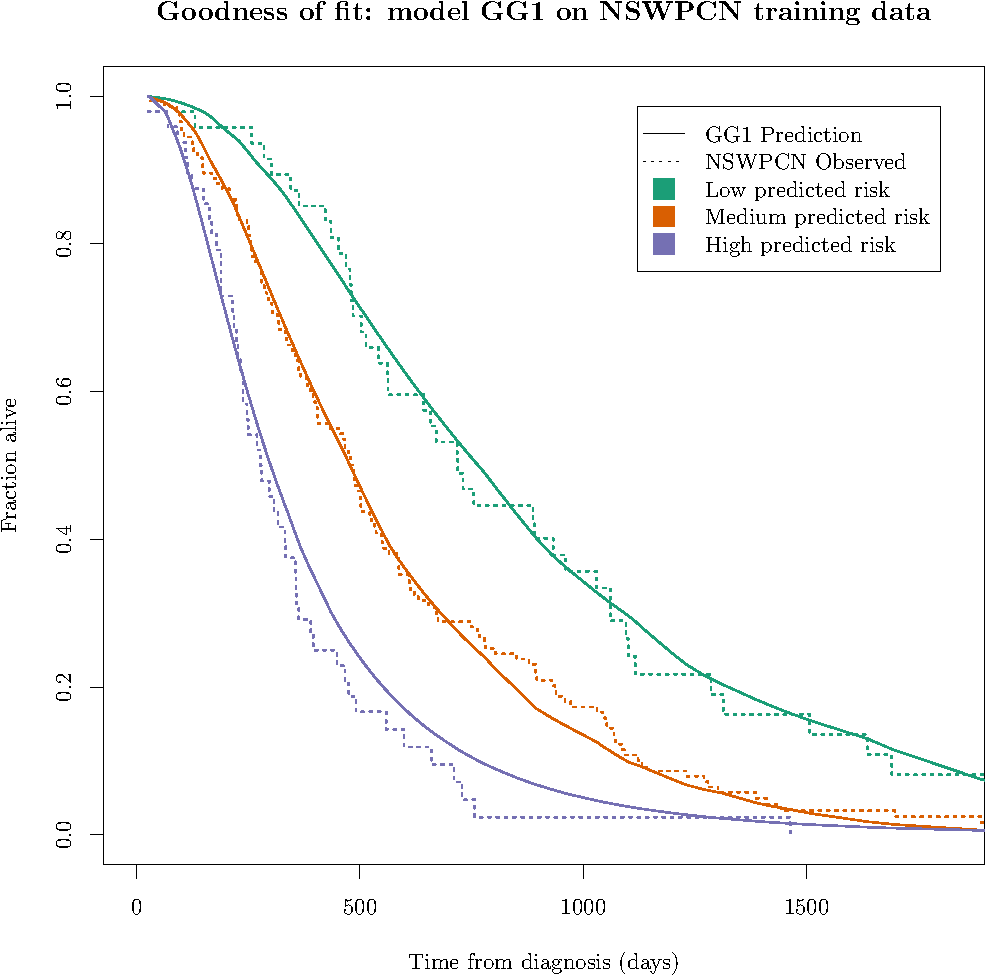
\includegraphics[width=\maxwidth]{figure/07-altman-4-nswpcn-1} 

}


\begin{kframe}\begin{alltt}
\hlkwd{summary}\hlstd{(}\hlkwd{coxph}\hlstd{(}\hlkwd{Surv}\hlstd{(data.nswpcn}\hlopt{$}\hlstd{Time, data.nswpcn}\hlopt{$}\hlstd{DSD)} \hlopt{~} \hlkwd{factor}\hlstd{(gg.groups.nswpcn)))}
\end{alltt}
\begin{verbatim}
## Call:
## coxph(formula = Surv(data.nswpcn$Time, data.nswpcn$DSD) ~ factor(gg.groups.nswpcn))
## 
##   n= 239, number of events= 230 
##    (1 observation deleted due to missingness)
## 
##                            coef exp(coef) se(coef)    z Pr(>|z|)
## factor(gg.groups.nswpcn)2 0.532     1.703    0.176 3.03   0.0025
## factor(gg.groups.nswpcn)3 1.328     3.775    0.219 6.06  1.3e-09
## 
##                           exp(coef) exp(-coef) lower .95 upper .95
## factor(gg.groups.nswpcn)2      1.70      0.587      1.21       2.4
## factor(gg.groups.nswpcn)3      3.78      0.265      2.46       5.8
## 
## Concordance= 0.618  (se = 0.019 )
## Rsquare= 0.138   (max possible= 1 )
## Likelihood ratio test= 35.5  on 2 df,   p=1.96e-08
## Wald test            = 37.9  on 2 df,   p=6.01e-09
## Score (logrank) test = 40.7  on 2 df,   p=1.46e-09
\end{verbatim}
\end{kframe}
\end{knitrout}

\begin{knitrout}
\definecolor{shadecolor}{rgb}{0.969, 0.969, 0.969}\color{fgcolor}\begin{kframe}
\begin{alltt}
\hlstd{mskcc_pre.groups.glasgow} \hlkwb{=} \hlkwd{cut}\hlstd{(mskcc_pre.linpred.glasgow,} \hlkwd{quantile}\hlstd{(mskcc_pre.linpred.glasgow, group_quantiles),} \hlkwc{labels} \hlstd{=} \hlnum{FALSE}\hlstd{)}
\hlstd{mskcc_post.groups.glasgow} \hlkwb{=} \hlkwd{cut}\hlstd{(mskcc_post.linpred.glasgow,} \hlkwd{quantile}\hlstd{(mskcc_post.linpred.glasgow, group_quantiles),} \hlkwc{labels} \hlstd{=} \hlnum{FALSE}\hlstd{)}
\hlstd{gg.groups.glasgow} \hlkwb{=} \hlkwd{cut}\hlstd{(gg.linpred.glasgow,} \hlkwd{quantile}\hlstd{(gg.linpred.glasgow, group_quantiles),} \hlkwc{labels} \hlstd{=} \hlnum{FALSE}\hlstd{)}

\hlstd{temp.km} \hlkwb{=} \hlkwd{survfit}\hlstd{(}\hlkwd{Surv}\hlstd{(data.glasgow}\hlopt{$}\hlstd{Time, data.glasgow}\hlopt{$}\hlstd{DSD)} \hlopt{~} \hlstd{gg.groups.glasgow,} \hlkwc{conf.int} \hlstd{=} \hlnum{1}\hlopt{-}\hlstd{temp.alpha)}
\hlstd{temp.km} \hlkwb{=} \hlkwd{data.frame}\hlstd{(}\hlkwc{surv} \hlstd{= temp.km}\hlopt{$}\hlstd{surv,} \hlkwc{group} \hlstd{=} \hlkwd{rep}\hlstd{(}\hlkwd{gsub}\hlstd{(}\hlstr{".*="}\hlstd{,} \hlstr{""}\hlstd{,} \hlkwd{names}\hlstd{(temp.km}\hlopt{$}\hlstd{strata)), temp.km}\hlopt{$}\hlstd{strata),} \hlkwc{time} \hlstd{= temp.km}\hlopt{$}\hlstd{time,} \hlkwc{upper} \hlstd{= temp.km}\hlopt{$}\hlstd{upper,} \hlkwc{lower} \hlstd{= temp.km}\hlopt{$}\hlstd{lower,} \hlkwc{est} \hlstd{=} \hlstr{"Glasgow Observed"}\hlstd{)}
\hlstd{temp.pred} \hlkwb{=} \hlkwd{summary}\hlstd{(fit.gg,} \hlkwc{newdata} \hlstd{= data.glasgow,} \hlkwc{ci} \hlstd{=} \hlnum{FALSE}\hlstd{)}
\hlstd{temp.pred.times} \hlkwb{=} \hlstd{temp.pred[[}\hlnum{1}\hlstd{]][,}\hlnum{1}\hlstd{]}
\hlstd{temp.pred.ests} \hlkwb{=} \hlkwd{sapply}\hlstd{(temp.pred,} \hlkwa{function}\hlstd{(}\hlkwc{x}\hlstd{) x[,}\hlnum{2}\hlstd{])}
\hlstd{temp.pred.ests} \hlkwb{=} \hlkwd{tapply}\hlstd{(}\hlnum{1}\hlopt{:}\hlkwd{ncol}\hlstd{(temp.pred.ests), gg.groups.glasgow,} \hlkwa{function}\hlstd{(}\hlkwc{is}\hlstd{)} \hlkwd{apply}\hlstd{(temp.pred.ests[,is],} \hlnum{1}\hlstd{, quantile,} \hlkwc{probs} \hlstd{=} \hlkwd{c}\hlstd{(temp.alpha}\hlopt{/}\hlnum{2}\hlstd{,} \hlnum{0.5}\hlstd{,} \hlnum{1}\hlopt{-}\hlstd{temp.alpha}\hlopt{/}\hlnum{2}\hlstd{),} \hlkwc{na.rm} \hlstd{=} \hlnum{TRUE}\hlstd{))}
\hlstd{temp.pred.lower} \hlkwb{=} \hlkwd{sapply}\hlstd{(temp.pred.ests,} \hlkwa{function}\hlstd{(}\hlkwc{x}\hlstd{) x[}\hlnum{1}\hlstd{,])}
\hlstd{temp.pred.meds} \hlkwb{=} \hlkwd{sapply}\hlstd{(temp.pred.ests,} \hlkwa{function}\hlstd{(}\hlkwc{x}\hlstd{) x[}\hlnum{2}\hlstd{,])}
\hlstd{temp.pred.upper} \hlkwb{=} \hlkwd{sapply}\hlstd{(temp.pred.ests,} \hlkwa{function}\hlstd{(}\hlkwc{x}\hlstd{) x[}\hlnum{3}\hlstd{,])}
\hlstd{temp.pred} \hlkwb{=} \hlkwd{data.frame}\hlstd{(}\hlkwc{surv} \hlstd{=} \hlkwd{as.vector}\hlstd{(temp.pred.meds),} \hlkwc{group} \hlstd{=} \hlkwd{rep}\hlstd{(}\hlkwd{colnames}\hlstd{(temp.pred.meds),} \hlkwc{each} \hlstd{=} \hlkwd{nrow}\hlstd{(temp.pred.meds)),} \hlkwc{time} \hlstd{= temp.pred.times,} \hlkwc{upper} \hlstd{=} \hlkwd{as.vector}\hlstd{(temp.pred.upper),} \hlkwc{lower} \hlstd{=} \hlkwd{as.vector}\hlstd{(temp.pred.lower),} \hlkwc{est} \hlstd{=} \hlstr{"GG1 Prediction"}\hlstd{)}
\hlstd{temp.data} \hlkwb{=} \hlkwd{rbind}\hlstd{(temp.km, temp.pred)}
\hlstd{temp.predpre.12mo} \hlkwb{=} \hlkwd{simplify2array}\hlstd{(}\hlkwd{tapply}\hlstd{(mskcc_pre.12mo.glasgow, mskcc_pre.groups.glasgow, quantile,} \hlkwc{probs} \hlstd{=} \hlkwd{c}\hlstd{(temp.alpha}\hlopt{/}\hlnum{2}\hlstd{,} \hlnum{0.5}\hlstd{,} \hlnum{1}\hlopt{-}\hlstd{temp.alpha}\hlopt{/}\hlnum{2}\hlstd{),} \hlkwc{na.rm} \hlstd{=} \hlnum{TRUE}\hlstd{))}
\hlstd{temp.predpre.24mo} \hlkwb{=} \hlkwd{simplify2array}\hlstd{(}\hlkwd{tapply}\hlstd{(mskcc_pre.24mo.glasgow, mskcc_pre.groups.glasgow, quantile,} \hlkwc{probs} \hlstd{=} \hlkwd{c}\hlstd{(temp.alpha}\hlopt{/}\hlnum{2}\hlstd{,} \hlnum{0.5}\hlstd{,} \hlnum{1}\hlopt{-}\hlstd{temp.alpha}\hlopt{/}\hlnum{2}\hlstd{),} \hlkwc{na.rm} \hlstd{=} \hlnum{TRUE}\hlstd{))}
\hlstd{temp.predpre.36mo} \hlkwb{=} \hlkwd{simplify2array}\hlstd{(}\hlkwd{tapply}\hlstd{(mskcc_pre.36mo.glasgow, mskcc_pre.groups.glasgow, quantile,} \hlkwc{probs} \hlstd{=} \hlkwd{c}\hlstd{(temp.alpha}\hlopt{/}\hlnum{2}\hlstd{,} \hlnum{0.5}\hlstd{,} \hlnum{1}\hlopt{-}\hlstd{temp.alpha}\hlopt{/}\hlnum{2}\hlstd{),} \hlkwc{na.rm} \hlstd{=} \hlnum{TRUE}\hlstd{))}
\hlstd{temp.predpost.12mo} \hlkwb{=} \hlkwd{simplify2array}\hlstd{(}\hlkwd{tapply}\hlstd{(mskcc_post.12mo.glasgow, mskcc_post.groups.glasgow, quantile,} \hlkwc{probs} \hlstd{=} \hlkwd{c}\hlstd{(temp.alpha}\hlopt{/}\hlnum{2}\hlstd{,} \hlnum{0.5}\hlstd{,} \hlnum{1}\hlopt{-}\hlstd{temp.alpha}\hlopt{/}\hlnum{2}\hlstd{),} \hlkwc{na.rm} \hlstd{=} \hlnum{TRUE}\hlstd{))}
\hlstd{temp.predpost.24mo} \hlkwb{=} \hlkwd{simplify2array}\hlstd{(}\hlkwd{tapply}\hlstd{(mskcc_post.24mo.glasgow, mskcc_post.groups.glasgow, quantile,} \hlkwc{probs} \hlstd{=} \hlkwd{c}\hlstd{(temp.alpha}\hlopt{/}\hlnum{2}\hlstd{,} \hlnum{0.5}\hlstd{,} \hlnum{1}\hlopt{-}\hlstd{temp.alpha}\hlopt{/}\hlnum{2}\hlstd{),} \hlkwc{na.rm} \hlstd{=} \hlnum{TRUE}\hlstd{))}
\hlstd{temp.predpost.36mo} \hlkwb{=} \hlkwd{simplify2array}\hlstd{(}\hlkwd{tapply}\hlstd{(mskcc_post.36mo.glasgow, mskcc_post.groups.glasgow, quantile,} \hlkwc{probs} \hlstd{=} \hlkwd{c}\hlstd{(temp.alpha}\hlopt{/}\hlnum{2}\hlstd{,} \hlnum{0.5}\hlstd{,} \hlnum{1}\hlopt{-}\hlstd{temp.alpha}\hlopt{/}\hlnum{2}\hlstd{),} \hlkwc{na.rm} \hlstd{=} \hlnum{TRUE}\hlstd{))}
\hlstd{temp.data2} \hlkwb{=} \hlkwd{data.frame}\hlstd{(}
        \hlkwc{surv} \hlstd{=} \hlkwd{c}\hlstd{(temp.predpre.12mo[}\hlnum{2}\hlstd{,], temp.predpre.24mo[}\hlnum{2}\hlstd{,], temp.predpre.36mo[}\hlnum{2}\hlstd{,], temp.predpost.12mo[}\hlnum{2}\hlstd{,], temp.predpost.24mo[}\hlnum{2}\hlstd{,], temp.predpost.36mo[}\hlnum{2}\hlstd{,]),}
        \hlkwc{group} \hlstd{=} \hlkwd{factor}\hlstd{(}\hlkwd{rep}\hlstd{(}\hlkwd{sort}\hlstd{(}\hlkwd{unique}\hlstd{(mskcc_pre.groups.glasgow)),} \hlnum{6}\hlstd{)),}
        \hlkwc{time} \hlstd{=} \hlkwd{rep}\hlstd{(}\hlkwd{c}\hlstd{(}\hlnum{12}\hlstd{,} \hlnum{24}\hlstd{,} \hlnum{36}\hlstd{)}\hlopt{/}\hlnum{12}\hlopt{*}\hlnum{365.25}\hlstd{,} \hlkwc{each} \hlstd{=} \hlnum{3}\hlstd{),}
        \hlkwc{upper} \hlstd{=} \hlkwd{c}\hlstd{(temp.predpre.12mo[}\hlnum{3}\hlstd{,], temp.predpre.24mo[}\hlnum{3}\hlstd{,], temp.predpre.36mo[}\hlnum{3}\hlstd{,], temp.predpost.12mo[}\hlnum{3}\hlstd{,], temp.predpost.24mo[}\hlnum{3}\hlstd{,], temp.predpost.36mo[}\hlnum{3}\hlstd{,]),}
        \hlkwc{lower} \hlstd{=} \hlkwd{c}\hlstd{(temp.predpre.12mo[}\hlnum{1}\hlstd{,], temp.predpre.24mo[}\hlnum{1}\hlstd{,], temp.predpre.36mo[}\hlnum{1}\hlstd{,], temp.predpost.12mo[}\hlnum{1}\hlstd{,], temp.predpost.24mo[}\hlnum{1}\hlstd{,], temp.predpost.36mo[}\hlnum{1}\hlstd{,]),}
        \hlkwc{est} \hlstd{=} \hlkwd{rep}\hlstd{(}\hlkwd{c}\hlstd{(}\hlstr{"MSKCC Preoperative"}\hlstd{,} \hlstr{"MSKCC Postoperative"}\hlstd{),} \hlkwc{each} \hlstd{=} \hlnum{9}\hlstd{))}
\hlcom{# ggplot(temp.data, aes(x = time, y = surv, colour = group, fill = group, ymax = upper, ymin = lower, lty = est)) + }
\hlcom{# 	geom_step() + }
\hlcom{# 	xlim(0, 5*365) + }
\hlcom{# 	geom_line(data = temp.data2) + }
\hlcom{# 	labs(title = "Goodness of fit: model GG1 on Glasgow validation data", x = "Time from diagnosis (days)", y = "Fraction alive", colour = "Risk group", lty = "Data")}

\hlkwd{plot}\hlstd{(}\hlnum{0} \hlopt{~} \hlnum{0}\hlstd{,} \hlkwc{type} \hlstd{=} \hlstr{"n"}\hlstd{,} \hlkwc{xlim} \hlstd{=} \hlkwd{c}\hlstd{(}\hlnum{0}\hlstd{,} \hlnum{5}\hlopt{*}\hlnum{365}\hlstd{),} \hlkwc{ylim} \hlstd{=} \hlkwd{c}\hlstd{(}\hlnum{0}\hlstd{,} \hlnum{1}\hlstd{),} \hlkwc{main} \hlstd{=} \hlstr{"Goodness of fit: model GG1 on Glasgow validation data"}\hlstd{,} \hlkwc{xlab} \hlstd{=} \hlstr{"Time from diagnosis (days)"}\hlstd{,} \hlkwc{ylab} \hlstd{=} \hlstr{"Fraction alive"}\hlstd{)}
\hlstd{temp.pal} \hlkwb{=} \hlkwd{brewer.pal}\hlstd{(}\hlkwd{length}\hlstd{(}\hlkwd{unique}\hlstd{(gg.groups.glasgow)),} \hlstr{"Dark2"}\hlstd{)}
\hlkwd{names}\hlstd{(temp.pal)} \hlkwb{=} \hlkwd{sort}\hlstd{(}\hlkwd{unique}\hlstd{(gg.groups.glasgow))}
\hlkwa{for} \hlstd{(temp.i} \hlkwa{in} \hlkwd{factor}\hlstd{(}\hlkwd{sort}\hlstd{(}\hlkwd{unique}\hlstd{(gg.groups.glasgow))))}
\hlstd{\{}
        \hlkwd{lines}\hlstd{(surv} \hlopt{~} \hlstd{time, temp.data[}\hlkwd{as.character}\hlstd{(temp.data}\hlopt{$}\hlstd{group)} \hlopt{==} \hlkwd{as.character}\hlstd{(temp.i)} \hlopt{&} \hlstd{temp.data}\hlopt{$}\hlstd{est} \hlopt{==} \hlstr{"Glasgow Observed"}\hlstd{,],} \hlkwc{type} \hlstd{=} \hlstr{"s"}\hlstd{,} \hlkwc{lty} \hlstd{=} \hlstr{"dotted"}\hlstd{,} \hlkwc{col} \hlstd{= temp.pal[}\hlkwd{as.character}\hlstd{(temp.i)],} \hlkwc{lwd} \hlstd{=} \hlnum{2}\hlstd{)}
        \hlkwd{lines}\hlstd{(surv} \hlopt{~} \hlstd{time, temp.data[}\hlkwd{as.character}\hlstd{(temp.data}\hlopt{$}\hlstd{group)} \hlopt{==} \hlkwd{as.character}\hlstd{(temp.i)} \hlopt{&} \hlstd{temp.data}\hlopt{$}\hlstd{est} \hlopt{==} \hlstr{"GG1 Prediction"}\hlstd{,],} \hlkwc{type} \hlstd{=} \hlstr{"l"}\hlstd{,} \hlkwc{lty} \hlstd{=} \hlstr{"solid"}\hlstd{,} \hlkwc{col} \hlstd{= temp.pal[}\hlkwd{as.character}\hlstd{(temp.i)],} \hlkwc{lwd} \hlstd{=} \hlnum{2}\hlstd{)}
        \hlkwd{points}\hlstd{(surv} \hlopt{~} \hlstd{time, temp.data2[}\hlkwd{as.character}\hlstd{(temp.data2}\hlopt{$}\hlstd{group)} \hlopt{==} \hlkwd{as.character}\hlstd{(temp.i)} \hlopt{&} \hlstd{temp.data2}\hlopt{$}\hlstd{est} \hlopt{==} \hlstr{"MSKCC Preoperative"}\hlstd{,],} \hlkwc{pch} \hlstd{=} \hlnum{21}\hlstd{,} \hlkwc{col} \hlstd{= temp.pal[}\hlkwd{as.character}\hlstd{(temp.i)],} \hlkwc{cex} \hlstd{=} \hlnum{1.5}\hlstd{)}
        \hlkwd{points}\hlstd{(surv} \hlopt{~} \hlstd{time, temp.data2[}\hlkwd{as.character}\hlstd{(temp.data2}\hlopt{$}\hlstd{group)} \hlopt{==} \hlkwd{as.character}\hlstd{(temp.i)} \hlopt{&} \hlstd{temp.data2}\hlopt{$}\hlstd{est} \hlopt{==} \hlstr{"MSKCC Postoperative"}\hlstd{,],} \hlkwc{pch} \hlstd{=} \hlnum{19}\hlstd{,} \hlkwc{col} \hlstd{= temp.pal[}\hlkwd{as.character}\hlstd{(temp.i)],} \hlkwc{cex} \hlstd{=} \hlnum{1.5}\hlstd{)}
\hlstd{\}}
\hlkwd{legend}\hlstd{(}\hlstr{"topright"}\hlstd{,} \hlkwc{inset} \hlstd{=} \hlnum{0.05}\hlstd{,} \hlkwc{legend} \hlstd{=} \hlkwd{c}\hlstd{(}\hlstr{"GG1 Prediction"}\hlstd{,} \hlstr{"MSKCC Preoperative Prediction"}\hlstd{,} \hlstr{"MSKCC Postoperative Prediction"}\hlstd{,} \hlstr{"Glasgow Observed"}\hlstd{,} \hlstr{"Low predicted risk"}\hlstd{,} \hlstr{"Medium predicted risk"}\hlstd{,} \hlstr{"High predicted risk"}\hlstd{),} \hlkwc{lty} \hlstd{=} \hlkwd{c}\hlstd{(}\hlstr{"solid"}\hlstd{,} \hlnum{NA}\hlstd{,} \hlnum{NA}\hlstd{,} \hlstr{"dotted"}\hlstd{,} \hlnum{NA}\hlstd{,} \hlnum{NA}\hlstd{,} \hlnum{NA}\hlstd{),} \hlkwc{col} \hlstd{=} \hlkwd{c}\hlstd{(}\hlstr{"black"}\hlstd{,} \hlstr{"black"}\hlstd{,} \hlstr{"black"}\hlstd{,} \hlstr{"black"}\hlstd{, temp.pal[}\hlnum{1}\hlopt{:}\hlnum{3}\hlstd{]),} \hlkwc{pch} \hlstd{=} \hlkwd{c}\hlstd{(}\hlnum{NA}\hlstd{,} \hlnum{21}\hlstd{,} \hlnum{19}\hlstd{,} \hlnum{NA}\hlstd{,} \hlnum{15}\hlstd{,} \hlnum{15}\hlstd{,} \hlnum{15}\hlstd{),} \hlkwc{pt.cex} \hlstd{=} \hlkwd{c}\hlstd{(}\hlnum{1}\hlstd{,} \hlnum{1}\hlstd{,} \hlnum{1}\hlstd{,} \hlnum{1}\hlstd{,} \hlnum{2}\hlstd{,} \hlnum{2}\hlstd{,} \hlnum{2}\hlstd{))}
\end{alltt}
\end{kframe}

{\centering 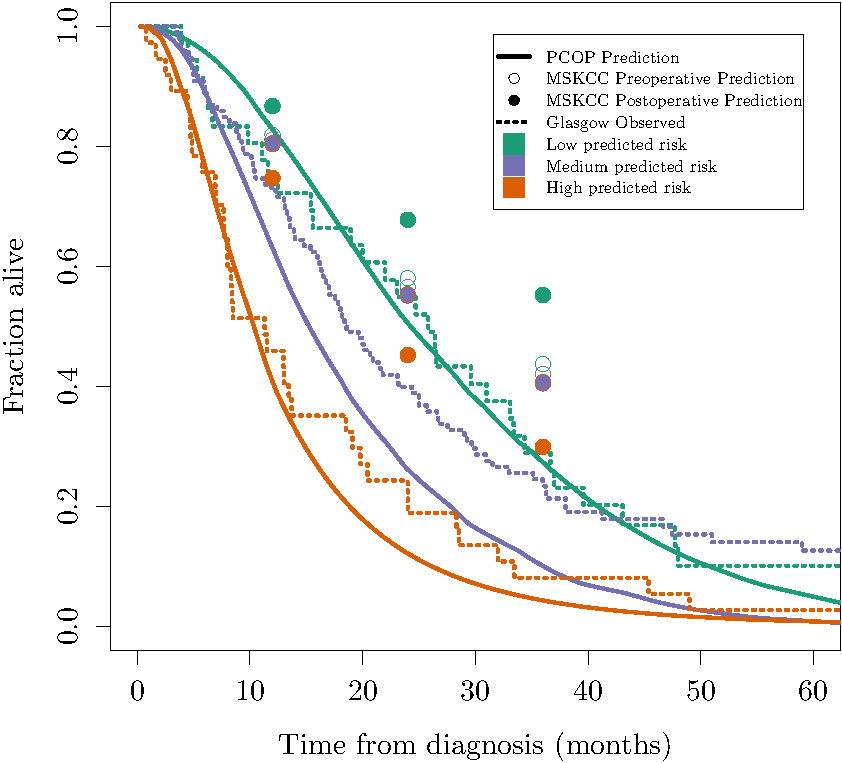
\includegraphics[width=\maxwidth]{figure/07-altman-4-glasgow-1} 

}


\begin{kframe}\begin{alltt}
\hlkwd{summary}\hlstd{(}\hlkwd{coxph}\hlstd{(}\hlkwd{Surv}\hlstd{(data.glasgow}\hlopt{$}\hlstd{Time, data.glasgow}\hlopt{$}\hlstd{DSD)} \hlopt{~} \hlkwd{factor}\hlstd{(gg.groups.glasgow)))}
\end{alltt}
\begin{verbatim}
## Call:
## coxph(formula = Surv(data.glasgow$Time, data.glasgow$DSD) ~ factor(gg.groups.glasgow))
## 
##   n= 188, number of events= 160 
##    (1 observation deleted due to missingness)
## 
##                              coef exp(coef) se(coef)    z Pr(>|z|)
## factor(gg.groups.glasgow)2 0.0794    1.0826   0.2074 0.38   0.7019
## factor(gg.groups.glasgow)3 0.6662    1.9468   0.2438 2.73   0.0063
## 
##                            exp(coef) exp(-coef) lower .95 upper .95
## factor(gg.groups.glasgow)2      1.08      0.924     0.721      1.63
## factor(gg.groups.glasgow)3      1.95      0.514     1.207      3.14
## 
## Concordance= 0.577  (se = 0.023 )
## Rsquare= 0.049   (max possible= 0.999 )
## Likelihood ratio test= 9.37  on 2 df,   p=0.00923
## Wald test            = 10.4  on 2 df,   p=0.00543
## Score (logrank) test = 10.8  on 2 df,   p=0.00463
\end{verbatim}
\begin{alltt}
\hlkwd{summary}\hlstd{(}\hlkwd{coxph}\hlstd{(}\hlkwd{Surv}\hlstd{(data.glasgow}\hlopt{$}\hlstd{Time, data.glasgow}\hlopt{$}\hlstd{DSD)} \hlopt{~} \hlkwd{factor}\hlstd{(mskcc_pre.groups.glasgow)))}
\end{alltt}
\begin{verbatim}
## Call:
## coxph(formula = Surv(data.glasgow$Time, data.glasgow$DSD) ~ factor(mskcc_pre.groups.glasgow))
## 
##   n= 188, number of events= 160 
##    (1 observation deleted due to missingness)
## 
##                                    coef exp(coef) se(coef)    z Pr(>|z|)
## factor(mskcc_pre.groups.glasgow)2 0.764     2.147    0.217 3.52  0.00043
## factor(mskcc_pre.groups.glasgow)3 0.762     2.143    0.260 2.93  0.00338
## 
##                                   exp(coef) exp(-coef) lower .95 upper .95
## factor(mskcc_pre.groups.glasgow)2      2.15      0.466      1.40      3.28
## factor(mskcc_pre.groups.glasgow)3      2.14      0.467      1.29      3.57
## 
## Concordance= 0.563  (se = 0.023 )
## Rsquare= 0.077   (max possible= 0.999 )
## Likelihood ratio test= 15.1  on 2 df,   p=0.000535
## Wald test            = 13.1  on 2 df,   p=0.00144
## Score (logrank) test = 13.6  on 2 df,   p=0.00109
\end{verbatim}
\begin{alltt}
\hlkwd{summary}\hlstd{(}\hlkwd{coxph}\hlstd{(}\hlkwd{Surv}\hlstd{(data.glasgow}\hlopt{$}\hlstd{Time, data.glasgow}\hlopt{$}\hlstd{DSD)} \hlopt{~} \hlkwd{factor}\hlstd{(mskcc_post.groups.glasgow)))}
\end{alltt}
\begin{verbatim}
## Call:
## coxph(formula = Surv(data.glasgow$Time, data.glasgow$DSD) ~ factor(mskcc_post.groups.glasgow))
## 
##   n= 188, number of events= 160 
##    (1 observation deleted due to missingness)
## 
##                                     coef exp(coef) se(coef)   z Pr(>|z|)
## factor(mskcc_post.groups.glasgow)2 0.631     1.879    0.218 2.9  0.00378
## factor(mskcc_post.groups.glasgow)3 0.990     2.691    0.261 3.8  0.00015
## 
##                                    exp(coef) exp(-coef) lower .95
## factor(mskcc_post.groups.glasgow)2      1.88      0.532      1.23
## factor(mskcc_post.groups.glasgow)3      2.69      0.372      1.61
##                                    upper .95
## factor(mskcc_post.groups.glasgow)2      2.88
## factor(mskcc_post.groups.glasgow)3      4.49
## 
## Concordance= 0.579  (se = 0.023 )
## Rsquare= 0.081   (max possible= 0.999 )
## Likelihood ratio test= 15.8  on 2 df,   p=0.000372
## Wald test            = 14.7  on 2 df,   p=0.00066
## Score (logrank) test = 15.3  on 2 df,   p=0.000484
\end{verbatim}
\end{kframe}
\end{knitrout}

\begin{knitrout}
\definecolor{shadecolor}{rgb}{0.969, 0.969, 0.969}\color{fgcolor}\begin{kframe}
\begin{alltt}
\hlstd{mskcc_pre.groups.apgi} \hlkwb{=} \hlkwd{cut}\hlstd{(mskcc_pre.linpred.apgi,} \hlkwd{quantile}\hlstd{(mskcc_pre.linpred.apgi, group_quantiles),} \hlkwc{labels} \hlstd{=} \hlnum{FALSE}\hlstd{)}
\hlstd{mskcc_post.groups.apgi} \hlkwb{=} \hlkwd{cut}\hlstd{(mskcc_post.linpred.apgi,} \hlkwd{quantile}\hlstd{(mskcc_post.linpred.apgi, group_quantiles),} \hlkwc{labels} \hlstd{=} \hlnum{FALSE}\hlstd{)}
\hlstd{gg.groups.apgi} \hlkwb{=} \hlkwd{cut}\hlstd{(gg.linpred.apgi,} \hlkwd{quantile}\hlstd{(gg.linpred.apgi, group_quantiles),} \hlkwc{labels} \hlstd{=} \hlnum{FALSE}\hlstd{)}

\hlstd{temp.km} \hlkwb{=} \hlkwd{survfit}\hlstd{(}\hlkwd{Surv}\hlstd{(data.apgi}\hlopt{$}\hlstd{Time, data.apgi}\hlopt{$}\hlstd{DSD)} \hlopt{~} \hlstd{gg.groups.apgi,} \hlkwc{conf.int} \hlstd{=} \hlnum{1}\hlopt{-}\hlstd{temp.alpha)}
\hlstd{temp.km} \hlkwb{=} \hlkwd{data.frame}\hlstd{(}\hlkwc{surv} \hlstd{= temp.km}\hlopt{$}\hlstd{surv,} \hlkwc{group} \hlstd{=} \hlkwd{rep}\hlstd{(}\hlkwd{gsub}\hlstd{(}\hlstr{".*="}\hlstd{,} \hlstr{""}\hlstd{,} \hlkwd{names}\hlstd{(temp.km}\hlopt{$}\hlstd{strata)), temp.km}\hlopt{$}\hlstd{strata),} \hlkwc{time} \hlstd{= temp.km}\hlopt{$}\hlstd{time,} \hlkwc{upper} \hlstd{= temp.km}\hlopt{$}\hlstd{upper,} \hlkwc{lower} \hlstd{= temp.km}\hlopt{$}\hlstd{lower,} \hlkwc{est} \hlstd{=} \hlstr{"APGI Observed"}\hlstd{)}
\hlstd{temp.pred} \hlkwb{=} \hlkwd{summary}\hlstd{(fit.gg,} \hlkwc{newdata} \hlstd{= data.apgi,} \hlkwc{ci} \hlstd{=} \hlnum{FALSE}\hlstd{)}
\hlstd{temp.pred.times} \hlkwb{=} \hlstd{temp.pred[[}\hlnum{1}\hlstd{]][,}\hlnum{1}\hlstd{]}
\hlstd{temp.pred.ests} \hlkwb{=} \hlkwd{sapply}\hlstd{(temp.pred,} \hlkwa{function}\hlstd{(}\hlkwc{x}\hlstd{) x[,}\hlnum{2}\hlstd{])}
\hlstd{temp.pred.ests} \hlkwb{=} \hlkwd{tapply}\hlstd{(}\hlnum{1}\hlopt{:}\hlkwd{ncol}\hlstd{(temp.pred.ests), gg.groups.apgi,} \hlkwa{function}\hlstd{(}\hlkwc{is}\hlstd{)} \hlkwd{apply}\hlstd{(temp.pred.ests[,is],} \hlnum{1}\hlstd{, quantile,} \hlkwc{probs} \hlstd{=} \hlkwd{c}\hlstd{(temp.alpha}\hlopt{/}\hlnum{2}\hlstd{,} \hlnum{0.5}\hlstd{,} \hlnum{1}\hlopt{-}\hlstd{temp.alpha}\hlopt{/}\hlnum{2}\hlstd{),} \hlkwc{na.rm} \hlstd{=} \hlnum{TRUE}\hlstd{))}
\hlstd{temp.pred.lower} \hlkwb{=} \hlkwd{sapply}\hlstd{(temp.pred.ests,} \hlkwa{function}\hlstd{(}\hlkwc{x}\hlstd{) x[}\hlnum{1}\hlstd{,])}
\hlstd{temp.pred.meds} \hlkwb{=} \hlkwd{sapply}\hlstd{(temp.pred.ests,} \hlkwa{function}\hlstd{(}\hlkwc{x}\hlstd{) x[}\hlnum{2}\hlstd{,])}
\hlstd{temp.pred.upper} \hlkwb{=} \hlkwd{sapply}\hlstd{(temp.pred.ests,} \hlkwa{function}\hlstd{(}\hlkwc{x}\hlstd{) x[}\hlnum{3}\hlstd{,])}
\hlstd{temp.pred} \hlkwb{=} \hlkwd{data.frame}\hlstd{(}\hlkwc{surv} \hlstd{=} \hlkwd{as.vector}\hlstd{(temp.pred.meds),} \hlkwc{group} \hlstd{=} \hlkwd{rep}\hlstd{(}\hlkwd{colnames}\hlstd{(temp.pred.meds),} \hlkwc{each} \hlstd{=} \hlkwd{nrow}\hlstd{(temp.pred.meds)),} \hlkwc{time} \hlstd{= temp.pred.times,} \hlkwc{upper} \hlstd{=} \hlkwd{as.vector}\hlstd{(temp.pred.upper),} \hlkwc{lower} \hlstd{=} \hlkwd{as.vector}\hlstd{(temp.pred.lower),} \hlkwc{est} \hlstd{=} \hlstr{"GG1 Prediction"}\hlstd{)}
\hlstd{temp.data} \hlkwb{=} \hlkwd{rbind}\hlstd{(temp.km, temp.pred)}
\hlstd{temp.predpre.12mo} \hlkwb{=} \hlkwd{simplify2array}\hlstd{(}\hlkwd{tapply}\hlstd{(mskcc_pre.12mo.apgi, mskcc_pre.groups.apgi, quantile,} \hlkwc{probs} \hlstd{=} \hlkwd{c}\hlstd{(temp.alpha}\hlopt{/}\hlnum{2}\hlstd{,} \hlnum{0.5}\hlstd{,} \hlnum{1}\hlopt{-}\hlstd{temp.alpha}\hlopt{/}\hlnum{2}\hlstd{),} \hlkwc{na.rm} \hlstd{=} \hlnum{TRUE}\hlstd{))}
\hlstd{temp.predpre.24mo} \hlkwb{=} \hlkwd{simplify2array}\hlstd{(}\hlkwd{tapply}\hlstd{(mskcc_pre.24mo.apgi, mskcc_pre.groups.apgi, quantile,} \hlkwc{probs} \hlstd{=} \hlkwd{c}\hlstd{(temp.alpha}\hlopt{/}\hlnum{2}\hlstd{,} \hlnum{0.5}\hlstd{,} \hlnum{1}\hlopt{-}\hlstd{temp.alpha}\hlopt{/}\hlnum{2}\hlstd{),} \hlkwc{na.rm} \hlstd{=} \hlnum{TRUE}\hlstd{))}
\hlstd{temp.predpre.36mo} \hlkwb{=} \hlkwd{simplify2array}\hlstd{(}\hlkwd{tapply}\hlstd{(mskcc_pre.36mo.apgi, mskcc_pre.groups.apgi, quantile,} \hlkwc{probs} \hlstd{=} \hlkwd{c}\hlstd{(temp.alpha}\hlopt{/}\hlnum{2}\hlstd{,} \hlnum{0.5}\hlstd{,} \hlnum{1}\hlopt{-}\hlstd{temp.alpha}\hlopt{/}\hlnum{2}\hlstd{),} \hlkwc{na.rm} \hlstd{=} \hlnum{TRUE}\hlstd{))}
\hlstd{temp.predpost.12mo} \hlkwb{=} \hlkwd{simplify2array}\hlstd{(}\hlkwd{tapply}\hlstd{(mskcc_post.12mo.apgi, mskcc_post.groups.apgi, quantile,} \hlkwc{probs} \hlstd{=} \hlkwd{c}\hlstd{(temp.alpha}\hlopt{/}\hlnum{2}\hlstd{,} \hlnum{0.5}\hlstd{,} \hlnum{1}\hlopt{-}\hlstd{temp.alpha}\hlopt{/}\hlnum{2}\hlstd{),} \hlkwc{na.rm} \hlstd{=} \hlnum{TRUE}\hlstd{))}
\hlstd{temp.predpost.24mo} \hlkwb{=} \hlkwd{simplify2array}\hlstd{(}\hlkwd{tapply}\hlstd{(mskcc_post.24mo.apgi, mskcc_post.groups.apgi, quantile,} \hlkwc{probs} \hlstd{=} \hlkwd{c}\hlstd{(temp.alpha}\hlopt{/}\hlnum{2}\hlstd{,} \hlnum{0.5}\hlstd{,} \hlnum{1}\hlopt{-}\hlstd{temp.alpha}\hlopt{/}\hlnum{2}\hlstd{),} \hlkwc{na.rm} \hlstd{=} \hlnum{TRUE}\hlstd{))}
\hlstd{temp.predpost.36mo} \hlkwb{=} \hlkwd{simplify2array}\hlstd{(}\hlkwd{tapply}\hlstd{(mskcc_post.36mo.apgi, mskcc_post.groups.apgi, quantile,} \hlkwc{probs} \hlstd{=} \hlkwd{c}\hlstd{(temp.alpha}\hlopt{/}\hlnum{2}\hlstd{,} \hlnum{0.5}\hlstd{,} \hlnum{1}\hlopt{-}\hlstd{temp.alpha}\hlopt{/}\hlnum{2}\hlstd{),} \hlkwc{na.rm} \hlstd{=} \hlnum{TRUE}\hlstd{))}
\hlstd{temp.data2} \hlkwb{=} \hlkwd{data.frame}\hlstd{(}
        \hlkwc{surv} \hlstd{=} \hlkwd{c}\hlstd{(temp.predpre.12mo[}\hlnum{2}\hlstd{,], temp.predpre.24mo[}\hlnum{2}\hlstd{,], temp.predpre.36mo[}\hlnum{2}\hlstd{,], temp.predpost.12mo[}\hlnum{2}\hlstd{,], temp.predpost.24mo[}\hlnum{2}\hlstd{,], temp.predpost.36mo[}\hlnum{2}\hlstd{,]),}
        \hlkwc{group} \hlstd{=} \hlkwd{factor}\hlstd{(}\hlkwd{rep}\hlstd{(}\hlkwd{sort}\hlstd{(}\hlkwd{unique}\hlstd{(mskcc_pre.groups.apgi)),} \hlnum{6}\hlstd{)),}
        \hlkwc{time} \hlstd{=} \hlkwd{rep}\hlstd{(}\hlkwd{c}\hlstd{(}\hlnum{12}\hlstd{,} \hlnum{24}\hlstd{,} \hlnum{36}\hlstd{)}\hlopt{/}\hlnum{12}\hlopt{*}\hlnum{365.25}\hlstd{,} \hlkwc{each} \hlstd{=} \hlnum{3}\hlstd{),}
        \hlkwc{upper} \hlstd{=} \hlkwd{c}\hlstd{(temp.predpre.12mo[}\hlnum{3}\hlstd{,], temp.predpre.24mo[}\hlnum{3}\hlstd{,], temp.predpre.36mo[}\hlnum{3}\hlstd{,], temp.predpost.12mo[}\hlnum{3}\hlstd{,], temp.predpost.24mo[}\hlnum{3}\hlstd{,], temp.predpost.36mo[}\hlnum{3}\hlstd{,]),}
        \hlkwc{lower} \hlstd{=} \hlkwd{c}\hlstd{(temp.predpre.12mo[}\hlnum{1}\hlstd{,], temp.predpre.24mo[}\hlnum{1}\hlstd{,], temp.predpre.36mo[}\hlnum{1}\hlstd{,], temp.predpost.12mo[}\hlnum{1}\hlstd{,], temp.predpost.24mo[}\hlnum{1}\hlstd{,], temp.predpost.36mo[}\hlnum{1}\hlstd{,]),}
        \hlkwc{est} \hlstd{=} \hlkwd{rep}\hlstd{(}\hlkwd{c}\hlstd{(}\hlstr{"MSKCC Preoperative"}\hlstd{,} \hlstr{"MSKCC Postoperative"}\hlstd{),} \hlkwc{each} \hlstd{=} \hlnum{9}\hlstd{))}
\hlcom{# ggplot(temp.data, aes(x = time, y = surv, colour = group, fill = group, ymax = upper, ymin = lower, lty = est)) + }
\hlcom{# 	geom_step() + }
\hlcom{# 	xlim(0, 5*365) + }
\hlcom{# 	geom_line(data = temp.data2) + }
\hlcom{# 	labs(title = "Goodness of fit: model GG1 on APGI validation data", x = "Time from diagnosis (days)", y = "Fraction alive", colour = "Risk group", lty = "Data")}

\hlkwd{plot}\hlstd{(}\hlnum{0} \hlopt{~} \hlnum{0}\hlstd{,} \hlkwc{type} \hlstd{=} \hlstr{"n"}\hlstd{,} \hlkwc{xlim} \hlstd{=} \hlkwd{c}\hlstd{(}\hlnum{0}\hlstd{,} \hlnum{5}\hlopt{*}\hlnum{365}\hlstd{),} \hlkwc{ylim} \hlstd{=} \hlkwd{c}\hlstd{(}\hlnum{0}\hlstd{,} \hlnum{1}\hlstd{),} \hlkwc{main} \hlstd{=} \hlstr{"Goodness of fit: model GG1 on APGI validation data"}\hlstd{,} \hlkwc{xlab} \hlstd{=} \hlstr{"Time from diagnosis (days)"}\hlstd{,} \hlkwc{ylab} \hlstd{=} \hlstr{"Fraction alive"}\hlstd{)}
\hlstd{temp.pal} \hlkwb{=} \hlkwd{brewer.pal}\hlstd{(}\hlkwd{length}\hlstd{(}\hlkwd{unique}\hlstd{(gg.groups.apgi)),} \hlstr{"Dark2"}\hlstd{)}
\hlkwd{names}\hlstd{(temp.pal)} \hlkwb{=} \hlkwd{sort}\hlstd{(}\hlkwd{unique}\hlstd{(gg.groups.apgi))}
\hlkwa{for} \hlstd{(temp.i} \hlkwa{in} \hlkwd{factor}\hlstd{(}\hlkwd{sort}\hlstd{(}\hlkwd{unique}\hlstd{(gg.groups.apgi))))}
\hlstd{\{}
        \hlkwd{lines}\hlstd{(surv} \hlopt{~} \hlstd{time, temp.data[}\hlkwd{as.character}\hlstd{(temp.data}\hlopt{$}\hlstd{group)} \hlopt{==} \hlkwd{as.character}\hlstd{(temp.i)} \hlopt{&} \hlstd{temp.data}\hlopt{$}\hlstd{est} \hlopt{==} \hlstr{"APGI Observed"}\hlstd{,],} \hlkwc{type} \hlstd{=} \hlstr{"s"}\hlstd{,} \hlkwc{lty} \hlstd{=} \hlstr{"dotted"}\hlstd{,} \hlkwc{col} \hlstd{= temp.pal[}\hlkwd{as.character}\hlstd{(temp.i)],} \hlkwc{lwd} \hlstd{=} \hlnum{2}\hlstd{)}
        \hlkwd{lines}\hlstd{(surv} \hlopt{~} \hlstd{time, temp.data[}\hlkwd{as.character}\hlstd{(temp.data}\hlopt{$}\hlstd{group)} \hlopt{==} \hlkwd{as.character}\hlstd{(temp.i)} \hlopt{&} \hlstd{temp.data}\hlopt{$}\hlstd{est} \hlopt{==} \hlstr{"GG1 Prediction"}\hlstd{,],} \hlkwc{type} \hlstd{=} \hlstr{"l"}\hlstd{,} \hlkwc{lty} \hlstd{=} \hlstr{"solid"}\hlstd{,} \hlkwc{col} \hlstd{= temp.pal[}\hlkwd{as.character}\hlstd{(temp.i)],} \hlkwc{lwd} \hlstd{=} \hlnum{2}\hlstd{)}
        \hlkwd{points}\hlstd{(surv} \hlopt{~} \hlstd{time, temp.data2[}\hlkwd{as.character}\hlstd{(temp.data2}\hlopt{$}\hlstd{group)} \hlopt{==} \hlkwd{as.character}\hlstd{(temp.i)} \hlopt{&} \hlstd{temp.data2}\hlopt{$}\hlstd{est} \hlopt{==} \hlstr{"MSKCC Preoperative"}\hlstd{,],} \hlkwc{pch} \hlstd{=} \hlnum{21}\hlstd{,} \hlkwc{col} \hlstd{= temp.pal[}\hlkwd{as.character}\hlstd{(temp.i)],} \hlkwc{cex} \hlstd{=} \hlnum{1.5}\hlstd{)}
        \hlkwd{points}\hlstd{(surv} \hlopt{~} \hlstd{time, temp.data2[}\hlkwd{as.character}\hlstd{(temp.data2}\hlopt{$}\hlstd{group)} \hlopt{==} \hlkwd{as.character}\hlstd{(temp.i)} \hlopt{&} \hlstd{temp.data2}\hlopt{$}\hlstd{est} \hlopt{==} \hlstr{"MSKCC Postoperative"}\hlstd{,],} \hlkwc{pch} \hlstd{=} \hlnum{19}\hlstd{,} \hlkwc{col} \hlstd{= temp.pal[}\hlkwd{as.character}\hlstd{(temp.i)],} \hlkwc{cex} \hlstd{=} \hlnum{1.5}\hlstd{)}
\hlstd{\}}
\hlkwd{legend}\hlstd{(}\hlstr{"topright"}\hlstd{,} \hlkwc{inset} \hlstd{=} \hlnum{0.05}\hlstd{,} \hlkwc{legend} \hlstd{=} \hlkwd{c}\hlstd{(}\hlstr{"GG1 Prediction"}\hlstd{,} \hlstr{"MSKCC Preoperative Prediction"}\hlstd{,} \hlstr{"MSKCC Postoperative Prediction"}\hlstd{,} \hlstr{"APGI Observed"}\hlstd{,} \hlstr{"Low predicted risk"}\hlstd{,} \hlstr{"Medium predicted risk"}\hlstd{,} \hlstr{"High predicted risk"}\hlstd{),} \hlkwc{lty} \hlstd{=} \hlkwd{c}\hlstd{(}\hlstr{"solid"}\hlstd{,} \hlnum{NA}\hlstd{,} \hlnum{NA}\hlstd{,} \hlstr{"dotted"}\hlstd{,} \hlnum{NA}\hlstd{,} \hlnum{NA}\hlstd{,} \hlnum{NA}\hlstd{),} \hlkwc{col} \hlstd{=} \hlkwd{c}\hlstd{(}\hlstr{"black"}\hlstd{,} \hlstr{"black"}\hlstd{,} \hlstr{"black"}\hlstd{,} \hlstr{"black"}\hlstd{, temp.pal[}\hlnum{1}\hlopt{:}\hlnum{3}\hlstd{]),} \hlkwc{pch} \hlstd{=} \hlkwd{c}\hlstd{(}\hlnum{NA}\hlstd{,} \hlnum{21}\hlstd{,} \hlnum{19}\hlstd{,} \hlnum{NA}\hlstd{,} \hlnum{15}\hlstd{,} \hlnum{15}\hlstd{,} \hlnum{15}\hlstd{),} \hlkwc{pt.cex} \hlstd{=} \hlkwd{c}\hlstd{(}\hlnum{1}\hlstd{,} \hlnum{1}\hlstd{,} \hlnum{1}\hlstd{,} \hlnum{1}\hlstd{,} \hlnum{2}\hlstd{,} \hlnum{2}\hlstd{,} \hlnum{2}\hlstd{))}
\end{alltt}
\end{kframe}

{\centering 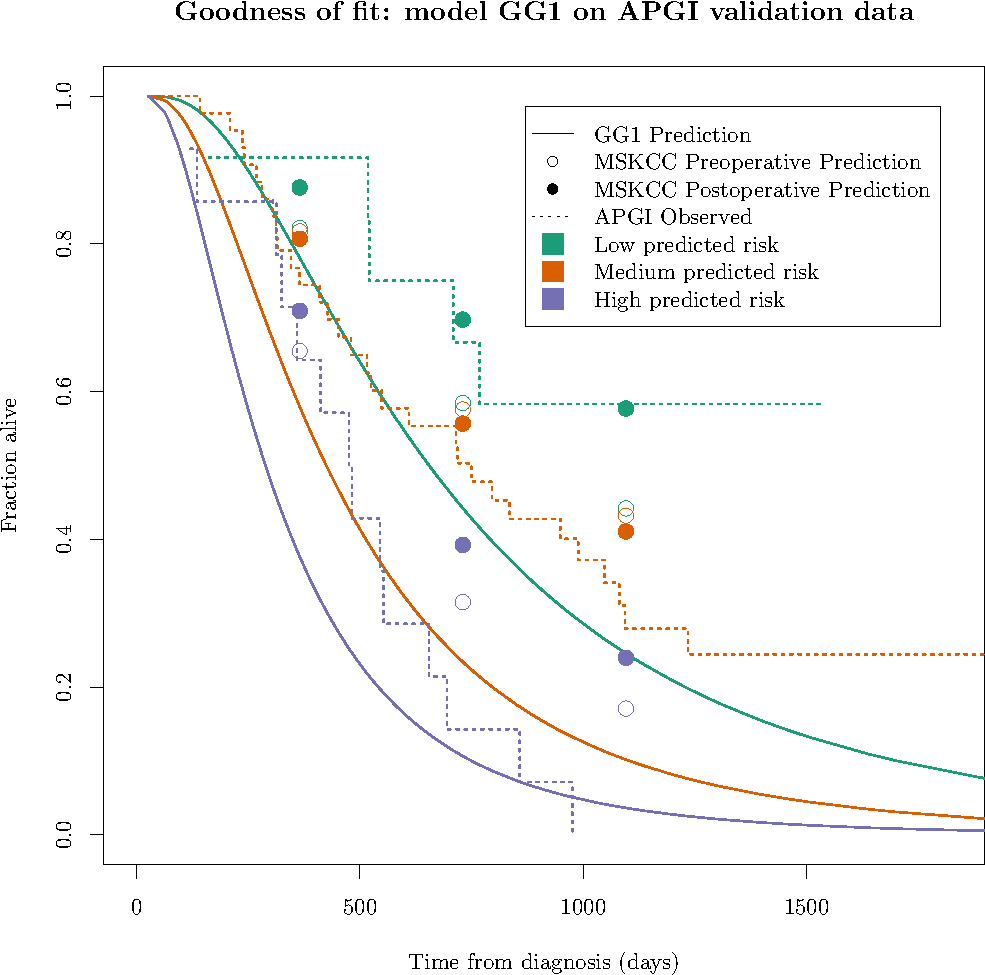
\includegraphics[width=\maxwidth]{figure/07-altman-4-apgi-1} 

}


\begin{kframe}\begin{alltt}
\hlkwd{summary}\hlstd{(}\hlkwd{coxph}\hlstd{(}\hlkwd{Surv}\hlstd{(data.apgi}\hlopt{$}\hlstd{Time, data.apgi}\hlopt{$}\hlstd{DSD)} \hlopt{~} \hlkwd{factor}\hlstd{(gg.groups.apgi)))}
\end{alltt}
\begin{verbatim}
## Call:
## coxph(formula = Surv(data.apgi$Time, data.apgi$DSD) ~ factor(gg.groups.apgi))
## 
##   n= 72, number of events= 50 
##    (3 observations deleted due to missingness)
## 
##                          coef exp(coef) se(coef)    z Pr(>|z|)
## factor(gg.groups.apgi)2 0.784     2.190    0.484 1.62   0.1051
## factor(gg.groups.apgi)3 1.689     5.413    0.533 3.17   0.0015
## 
##                         exp(coef) exp(-coef) lower .95 upper .95
## factor(gg.groups.apgi)2      2.19      0.457     0.849      5.65
## factor(gg.groups.apgi)3      5.41      0.185     1.905     15.38
## 
## Concordance= 0.609  (se = 0.039 )
## Rsquare= 0.153   (max possible= 0.993 )
## Likelihood ratio test= 11.9  on 2 df,   p=0.00254
## Wald test            = 12  on 2 df,   p=0.00249
## Score (logrank) test = 13.4  on 2 df,   p=0.00124
\end{verbatim}
\begin{alltt}
\hlkwd{summary}\hlstd{(}\hlkwd{coxph}\hlstd{(}\hlkwd{Surv}\hlstd{(data.apgi}\hlopt{$}\hlstd{Time, data.apgi}\hlopt{$}\hlstd{DSD)} \hlopt{~} \hlkwd{factor}\hlstd{(mskcc_pre.groups.apgi)))}
\end{alltt}
\begin{verbatim}
## Call:
## coxph(formula = Surv(data.apgi$Time, data.apgi$DSD) ~ factor(mskcc_pre.groups.apgi))
## 
##   n= 74, number of events= 50 
##    (1 observation deleted due to missingness)
## 
##                                  coef exp(coef) se(coef)     z Pr(>|z|)
## factor(mskcc_pre.groups.apgi)2 -0.412     0.662    0.367 -1.12     0.26
## factor(mskcc_pre.groups.apgi)3 -0.058     0.944    0.449 -0.13     0.90
## 
##                                exp(coef) exp(-coef) lower .95 upper .95
## factor(mskcc_pre.groups.apgi)2     0.662       1.51     0.322      1.36
## factor(mskcc_pre.groups.apgi)3     0.944       1.06     0.392      2.27
## 
## Concordance= 0.559  (se = 0.037 )
## Rsquare= 0.023   (max possible= 0.993 )
## Likelihood ratio test= 1.7  on 2 df,   p=0.428
## Wald test            = 1.75  on 2 df,   p=0.417
## Score (logrank) test = 1.77  on 2 df,   p=0.412
\end{verbatim}
\begin{alltt}
\hlkwd{summary}\hlstd{(}\hlkwd{coxph}\hlstd{(}\hlkwd{Surv}\hlstd{(data.apgi}\hlopt{$}\hlstd{Time, data.apgi}\hlopt{$}\hlstd{DSD)} \hlopt{~} \hlkwd{factor}\hlstd{(mskcc_post.groups.apgi)))}
\end{alltt}
\begin{verbatim}
## Call:
## coxph(formula = Surv(data.apgi$Time, data.apgi$DSD) ~ factor(mskcc_post.groups.apgi))
## 
##   n= 74, number of events= 51 
##    (1 observation deleted due to missingness)
## 
##                                  coef exp(coef) se(coef)    z Pr(>|z|)
## factor(mskcc_post.groups.apgi)2 1.526     4.598    0.531 2.87   0.0041
## factor(mskcc_post.groups.apgi)3 1.812     6.125    0.576 3.15   0.0016
## 
##                                 exp(coef) exp(-coef) lower .95 upper .95
## factor(mskcc_post.groups.apgi)2      4.60      0.217      1.62      13.0
## factor(mskcc_post.groups.apgi)3      6.12      0.163      1.98      18.9
## 
## Concordance= 0.624  (se = 0.04 )
## Rsquare= 0.184   (max possible= 0.993 )
## Likelihood ratio test= 15.1  on 2 df,   p=0.000539
## Wald test            = 10.1  on 2 df,   p=0.00628
## Score (logrank) test = 12.3  on 2 df,   p=0.00208
\end{verbatim}
\end{kframe}
\end{knitrout}


Decision curve analysis.
\begin{knitrout}
\definecolor{shadecolor}{rgb}{0.969, 0.969, 0.969}\color{fgcolor}\begin{kframe}
\begin{alltt}
\hlkwd{source}\hlstd{(}\hlstr{"stdca.R"}\hlstd{)}
\hlstd{temp.data} \hlkwb{=} \hlkwd{data.frame}\hlstd{(}\hlkwc{Time} \hlstd{= data.glasgow}\hlopt{$}\hlstd{Time,} \hlkwc{DSD} \hlstd{= data.glasgow}\hlopt{$}\hlstd{DSD}\hlopt{*}\hlnum{1}\hlstd{,}
    \hlkwc{gg.1} \hlstd{=} \hlnum{1}\hlopt{-}\hlstd{gg.prob.glasgow[val.prob.times} \hlopt{==} \hlnum{365}\hlstd{,],} \hlkwc{gg.2} \hlstd{=} \hlnum{1}\hlopt{-}\hlstd{gg.prob.glasgow[val.prob.times} \hlopt{==} \hlnum{365}\hlopt{*}\hlnum{2}\hlstd{,],} \hlkwc{gg.3} \hlstd{=} \hlnum{1}\hlopt{-}\hlstd{gg.prob.glasgow[val.prob.times} \hlopt{==} \hlnum{365}\hlopt{*}\hlnum{3}\hlstd{,],}
    \hlkwc{mskcc.pre.1} \hlstd{=} \hlnum{1}\hlopt{-}\hlstd{mskcc_pre.12mo.glasgow,} \hlkwc{mskcc.pre.2} \hlstd{=} \hlnum{1}\hlopt{-}\hlstd{mskcc_pre.24mo.glasgow,} \hlkwc{mskcc.pre.3} \hlstd{=} \hlnum{1}\hlopt{-}\hlstd{mskcc_pre.36mo.glasgow,}
    \hlkwc{mskcc.post.1} \hlstd{=} \hlnum{1}\hlopt{-}\hlstd{mskcc_post.12mo.glasgow,} \hlkwc{mskcc.post.2} \hlstd{=} \hlnum{1}\hlopt{-}\hlstd{mskcc_post.24mo.glasgow,} \hlkwc{mskcc.post.3} \hlstd{=} \hlnum{1}\hlopt{-}\hlstd{mskcc_post.36mo.glasgow)}
\hlkwd{invisible}\hlstd{(}\hlkwd{stdca}\hlstd{(}\hlkwc{data} \hlstd{= temp.data,} \hlkwc{outcome} \hlstd{=} \hlstr{"DSD"}\hlstd{,} \hlkwc{ttoutcome} \hlstd{=} \hlstr{"Time"}\hlstd{,} \hlkwc{predictors} \hlstd{=} \hlkwd{c}\hlstd{(}\hlstr{"gg.1"}\hlstd{,} \hlstr{"mskcc.pre.1"}\hlstd{,} \hlstr{"mskcc.post.1"}\hlstd{),} \hlkwc{timepoint} \hlstd{=} \hlnum{365}\hlstd{,} \hlkwc{probability} \hlstd{=} \hlkwd{rep}\hlstd{(}\hlnum{TRUE}\hlstd{,} \hlnum{3}\hlstd{)))}
\end{alltt}
\begin{verbatim}
## [1] "gg.1: No observations with risk greater than 63% that have followup through the timepoint selected, and therefore net benefit not calculable in this range."        
## [2] "mskcc.pre.1: No observations with risk greater than 32%, and therefore net benefit not calculable in this range."                                                   
## [3] "mskcc.post.1: No observations with risk greater than 30% that have followup through the timepoint selected, and therefore net benefit not calculable in this range."
\end{verbatim}
\end{kframe}

{\centering 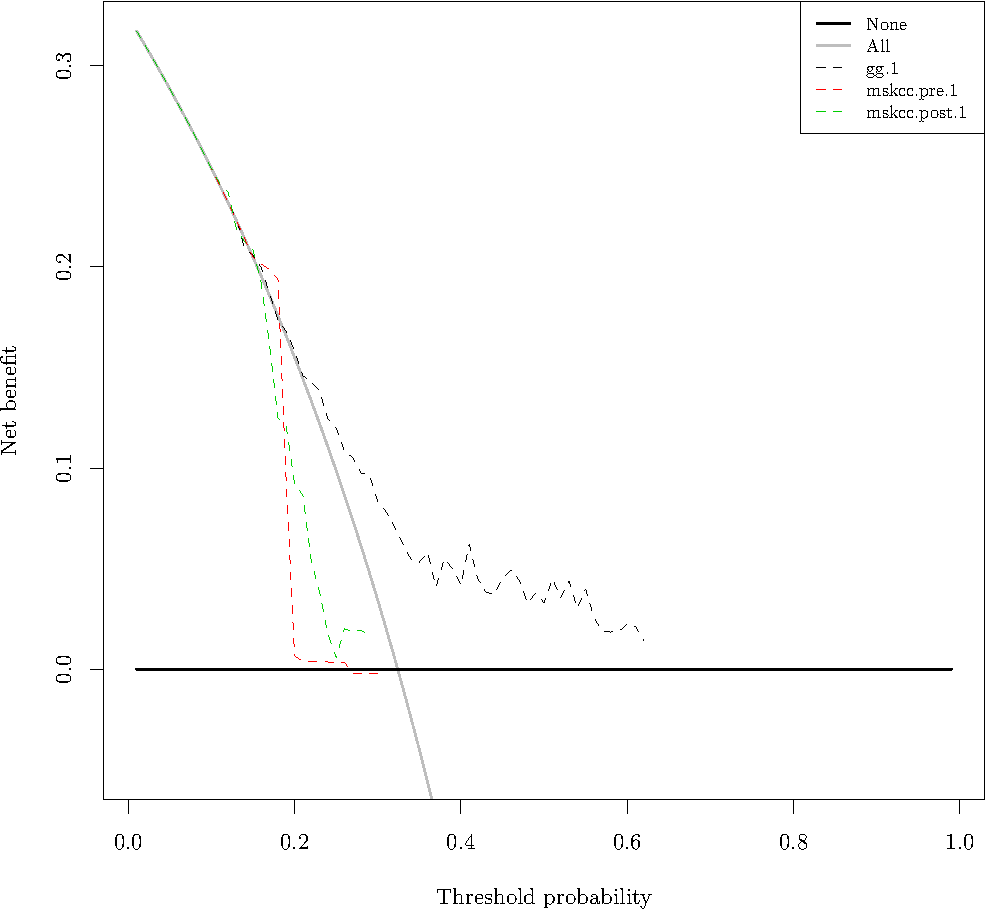
\includegraphics[width=\maxwidth]{figure/07-model-selection-dca-1} 

}


\begin{kframe}\begin{alltt}
\hlkwd{invisible}\hlstd{(}\hlkwd{stdca}\hlstd{(}\hlkwc{data} \hlstd{= temp.data,} \hlkwc{outcome} \hlstd{=} \hlstr{"DSD"}\hlstd{,} \hlkwc{ttoutcome} \hlstd{=} \hlstr{"Time"}\hlstd{,} \hlkwc{predictors} \hlstd{=} \hlkwd{c}\hlstd{(}\hlstr{"gg.2"}\hlstd{,} \hlstr{"mskcc.pre.2"}\hlstd{,} \hlstr{"mskcc.post.2"}\hlstd{),} \hlkwc{timepoint} \hlstd{=} \hlnum{365}\hlopt{*}\hlnum{2}\hlstd{,} \hlkwc{probability} \hlstd{=} \hlkwd{rep}\hlstd{(}\hlnum{TRUE}\hlstd{,} \hlnum{3}\hlstd{)))}
\end{alltt}
\begin{verbatim}
## [1] "gg.2: No observations with risk greater than 94% that have followup through the timepoint selected, and therefore net benefit not calculable in this range."        
## [2] "mskcc.pre.2: No observations with risk greater than 65%, and therefore net benefit not calculable in this range."                                                   
## [3] "mskcc.post.2: No observations with risk greater than 61% that have followup through the timepoint selected, and therefore net benefit not calculable in this range."
\end{verbatim}
\end{kframe}

{\centering 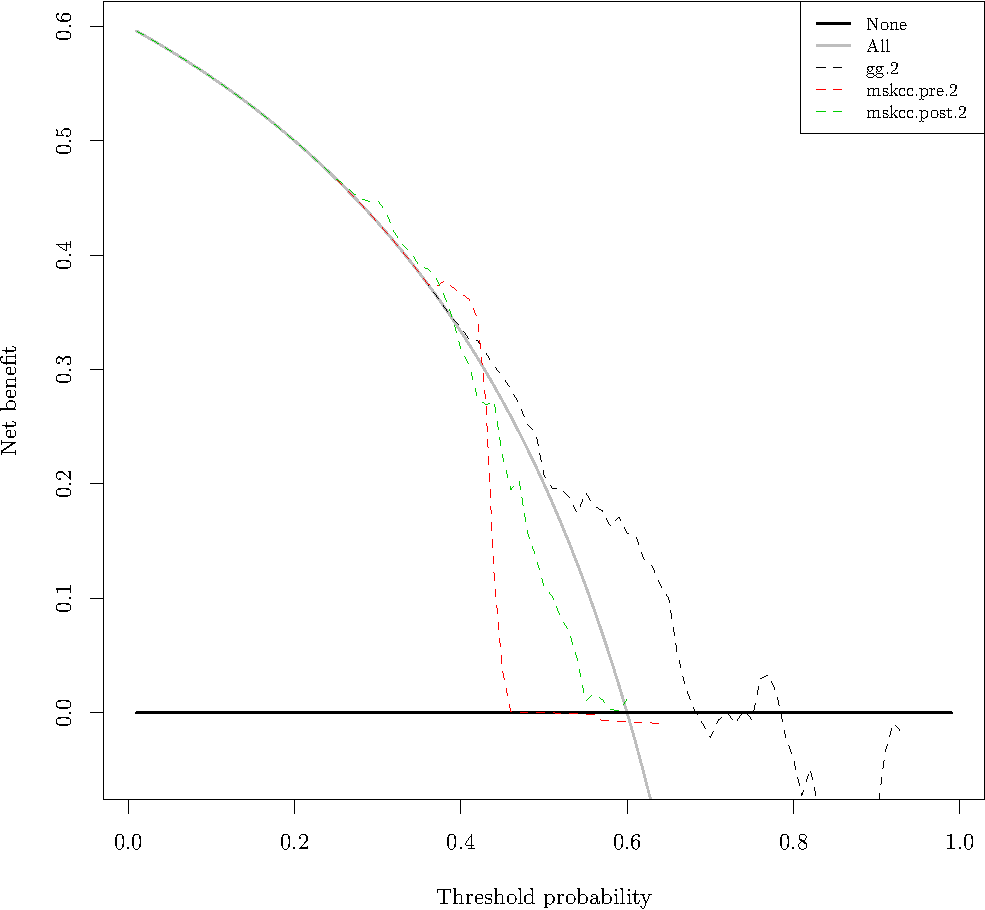
\includegraphics[width=\maxwidth]{figure/07-model-selection-dca-2} 

}


\begin{kframe}\begin{alltt}
\hlkwd{invisible}\hlstd{(}\hlkwd{stdca}\hlstd{(}\hlkwc{data} \hlstd{= temp.data,} \hlkwc{outcome} \hlstd{=} \hlstr{"DSD"}\hlstd{,} \hlkwc{ttoutcome} \hlstd{=} \hlstr{"Time"}\hlstd{,} \hlkwc{predictors} \hlstd{=} \hlkwd{c}\hlstd{(}\hlstr{"gg.3"}\hlstd{,} \hlstr{"mskcc.pre.3"}\hlstd{,} \hlstr{"mskcc.post.3"}\hlstd{),} \hlkwc{timepoint} \hlstd{=} \hlnum{365}\hlopt{*}\hlnum{3}\hlstd{,} \hlkwc{probability} \hlstd{=} \hlkwd{rep}\hlstd{(}\hlnum{TRUE}\hlstd{,} \hlnum{3}\hlstd{)))}
\end{alltt}
\begin{verbatim}
## [1] "mskcc.pre.3: No observations with risk greater than 80%, and therefore net benefit not calculable in this range."                                                   
## [2] "mskcc.post.3: No observations with risk greater than 77% that have followup through the timepoint selected, and therefore net benefit not calculable in this range."
\end{verbatim}
\end{kframe}

{\centering 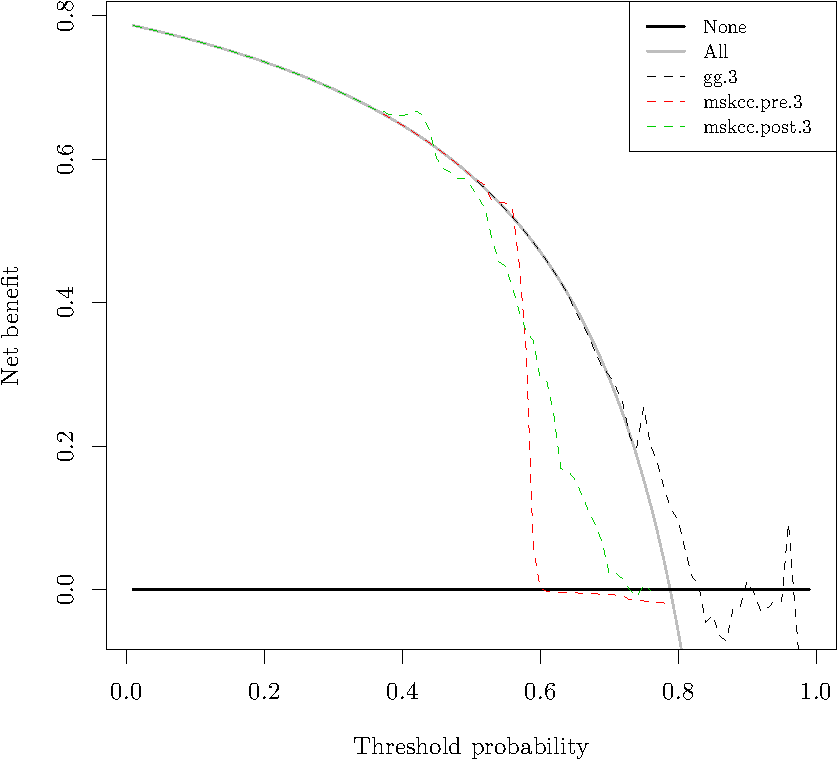
\includegraphics[width=\maxwidth]{figure/07-model-selection-dca-3} 

}


\begin{kframe}\begin{alltt}
\hlstd{temp.data} \hlkwb{=} \hlkwd{data.frame}\hlstd{(}\hlkwc{Time} \hlstd{= data.apgi}\hlopt{$}\hlstd{Time,} \hlkwc{DSD} \hlstd{= data.apgi}\hlopt{$}\hlstd{DSD}\hlopt{*}\hlnum{1}\hlstd{,}
    \hlkwc{gg.1} \hlstd{=} \hlnum{1}\hlopt{-}\hlstd{gg.prob.apgi[val.prob.times} \hlopt{==} \hlnum{365}\hlstd{,],} \hlkwc{gg.2} \hlstd{=} \hlnum{1}\hlopt{-}\hlstd{gg.prob.apgi[val.prob.times} \hlopt{==} \hlnum{365}\hlopt{*}\hlnum{2}\hlstd{,],} \hlkwc{gg.3} \hlstd{=} \hlnum{1}\hlopt{-}\hlstd{gg.prob.apgi[val.prob.times} \hlopt{==} \hlnum{365}\hlopt{*}\hlnum{3}\hlstd{,],}
    \hlkwc{mskcc.pre.1} \hlstd{=} \hlnum{1}\hlopt{-}\hlstd{mskcc_pre.12mo.apgi,} \hlkwc{mskcc.pre.2} \hlstd{=} \hlnum{1}\hlopt{-}\hlstd{mskcc_pre.24mo.apgi,} \hlkwc{mskcc.pre.3} \hlstd{=} \hlnum{1}\hlopt{-}\hlstd{mskcc_pre.36mo.apgi,}
    \hlkwc{mskcc.post.1} \hlstd{=} \hlnum{1}\hlopt{-}\hlstd{mskcc_post.12mo.apgi,} \hlkwc{mskcc.post.2} \hlstd{=} \hlnum{1}\hlopt{-}\hlstd{mskcc_post.24mo.apgi,} \hlkwc{mskcc.post.3} \hlstd{=} \hlnum{1}\hlopt{-}\hlstd{mskcc_post.36mo.apgi)}
\hlkwd{invisible}\hlstd{(}\hlkwd{stdca}\hlstd{(}\hlkwc{data} \hlstd{= temp.data,} \hlkwc{outcome} \hlstd{=} \hlstr{"DSD"}\hlstd{,} \hlkwc{ttoutcome} \hlstd{=} \hlstr{"Time"}\hlstd{,} \hlkwc{predictors} \hlstd{=} \hlkwd{c}\hlstd{(}\hlstr{"gg.1"}\hlstd{,} \hlstr{"mskcc.pre.1"}\hlstd{,} \hlstr{"mskcc.post.1"}\hlstd{),} \hlkwc{timepoint} \hlstd{=} \hlnum{365}\hlstd{,} \hlkwc{probability} \hlstd{=} \hlkwd{rep}\hlstd{(}\hlnum{TRUE}\hlstd{,} \hlnum{3}\hlstd{)))}
\end{alltt}
\begin{verbatim}
## [1] "gg.1: No observations with risk greater than 78%, and therefore net benefit not calculable in this range."        
## [2] "mskcc.pre.1: No observations with risk greater than 50%, and therefore net benefit not calculable in this range." 
## [3] "mskcc.post.1: No observations with risk greater than 50%, and therefore net benefit not calculable in this range."
\end{verbatim}
\end{kframe}

{\centering 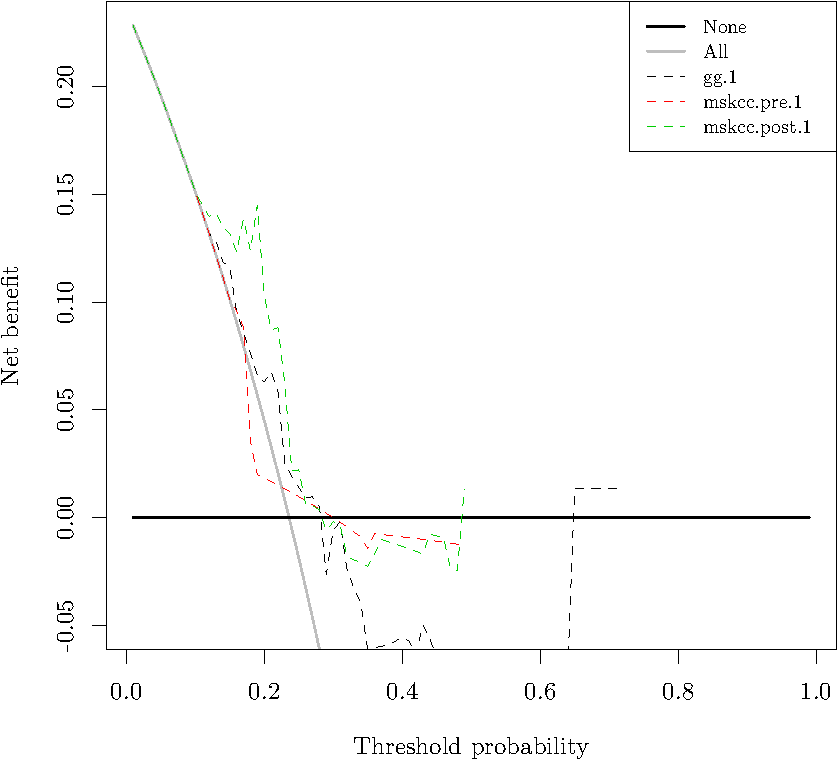
\includegraphics[width=\maxwidth]{figure/07-model-selection-dca-4} 

}


\begin{kframe}\begin{alltt}
\hlkwd{invisible}\hlstd{(}\hlkwd{stdca}\hlstd{(}\hlkwc{data} \hlstd{= temp.data,} \hlkwc{outcome} \hlstd{=} \hlstr{"DSD"}\hlstd{,} \hlkwc{ttoutcome} \hlstd{=} \hlstr{"Time"}\hlstd{,} \hlkwc{predictors} \hlstd{=} \hlkwd{c}\hlstd{(}\hlstr{"gg.2"}\hlstd{,} \hlstr{"mskcc.pre.2"}\hlstd{,} \hlstr{"mskcc.post.2"}\hlstd{),} \hlkwc{timepoint} \hlstd{=} \hlnum{365}\hlopt{*}\hlnum{2}\hlstd{,} \hlkwc{probability} \hlstd{=} \hlkwd{rep}\hlstd{(}\hlnum{TRUE}\hlstd{,} \hlnum{3}\hlstd{)))}
\end{alltt}
\begin{verbatim}
## [1] "gg.2: No observations with risk greater than 89% that have followup through the timepoint selected, and therefore net benefit not calculable in this range."        
## [2] "mskcc.pre.2: No observations with risk greater than 85%, and therefore net benefit not calculable in this range."                                                   
## [3] "mskcc.post.2: No observations with risk greater than 80% that have followup through the timepoint selected, and therefore net benefit not calculable in this range."
\end{verbatim}
\end{kframe}

{\centering 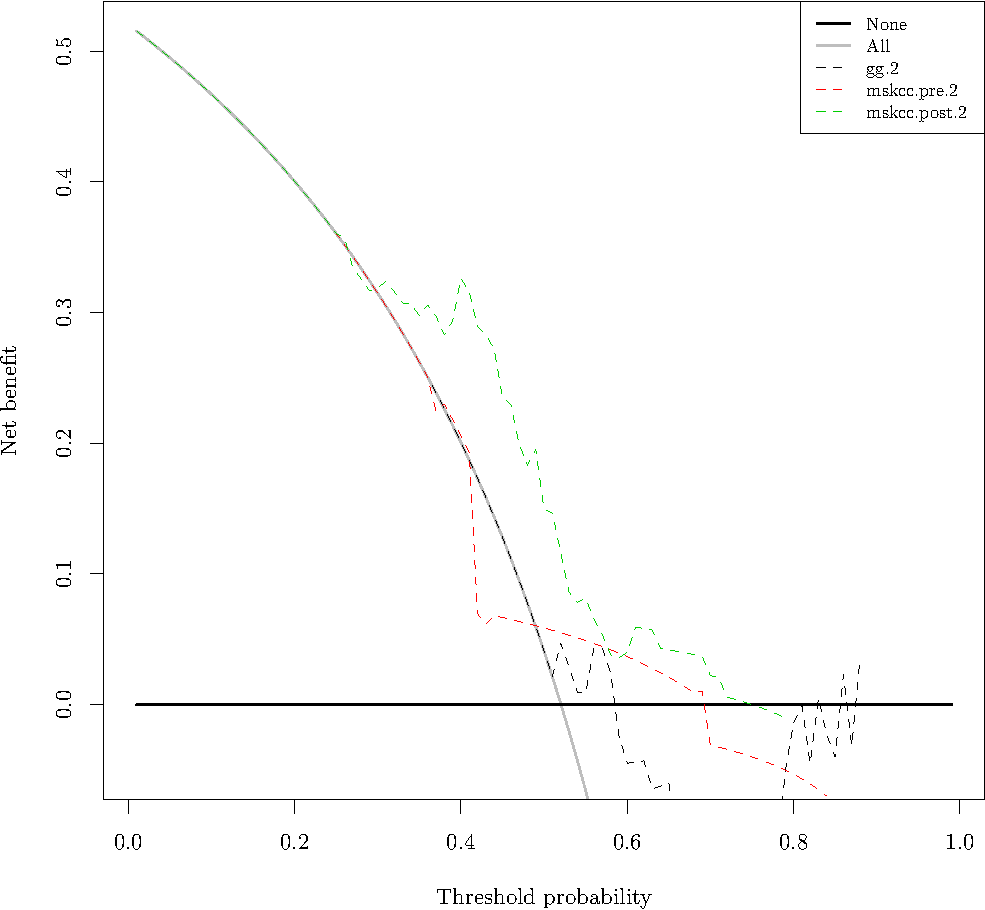
\includegraphics[width=\maxwidth]{figure/07-model-selection-dca-5} 

}


\begin{kframe}\begin{alltt}
\hlkwd{invisible}\hlstd{(}\hlkwd{stdca}\hlstd{(}\hlkwc{data} \hlstd{= temp.data,} \hlkwc{outcome} \hlstd{=} \hlstr{"DSD"}\hlstd{,} \hlkwc{ttoutcome} \hlstd{=} \hlstr{"Time"}\hlstd{,} \hlkwc{predictors} \hlstd{=} \hlkwd{c}\hlstd{(}\hlstr{"gg.3"}\hlstd{,} \hlstr{"mskcc.pre.3"}\hlstd{,} \hlstr{"mskcc.post.3"}\hlstd{),} \hlkwc{timepoint} \hlstd{=} \hlnum{365}\hlopt{*}\hlnum{3}\hlstd{,} \hlkwc{probability} \hlstd{=} \hlkwd{rep}\hlstd{(}\hlnum{TRUE}\hlstd{,} \hlnum{3}\hlstd{)))}
\end{alltt}
\begin{verbatim}
## [1] "gg.3: No observations with risk greater than 92% that have followup through the timepoint selected, and therefore net benefit not calculable in this range."        
## [2] "mskcc.pre.3: No observations with risk greater than 95%, and therefore net benefit not calculable in this range."                                                   
## [3] "mskcc.post.3: No observations with risk greater than 92% that have followup through the timepoint selected, and therefore net benefit not calculable in this range."
\end{verbatim}
\end{kframe}

{\centering 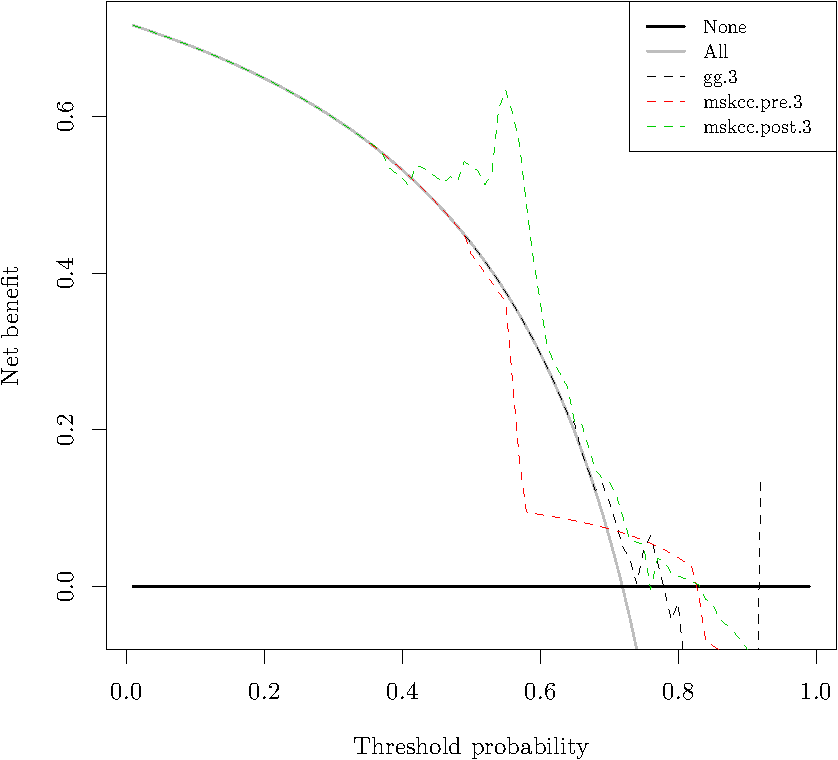
\includegraphics[width=\maxwidth]{figure/07-model-selection-dca-6} 

}



\end{knitrout}


\subsection{Brier score}
\begin{knitrout}
\definecolor{shadecolor}{rgb}{0.969, 0.969, 0.969}\color{fgcolor}\begin{kframe}
\begin{alltt}
\hlstd{calcIBS} \hlkwb{=} \hlkwa{function}\hlstd{(}\hlkwc{surv}\hlstd{,} \hlkwc{pred}\hlstd{,} \hlkwc{pred_times}\hlstd{,} \hlkwc{max_time}\hlstd{,} \hlkwc{min_time} \hlstd{=} \hlnum{0}\hlstd{)}
\hlstd{\{}
        \hlkwd{stopifnot}\hlstd{(}\hlkwd{nrow}\hlstd{(surv)} \hlopt{==} \hlkwd{nrow}\hlstd{(pred)} \hlopt{&&} \hlkwd{length}\hlstd{(pred_times)} \hlopt{==} \hlkwd{ncol}\hlstd{(pred))}

        \hlstd{n} \hlkwb{=} \hlkwd{nrow}\hlstd{(surv)}
        \hlstd{marg_survfit} \hlkwb{=} \hlkwd{survfit}\hlstd{(surv} \hlopt{~} \hlnum{1}\hlstd{)}
        \hlstd{marg_censfit} \hlkwb{=} \hlkwd{survfit}\hlstd{(}\hlkwd{Surv}\hlstd{(surv[,}\hlnum{1}\hlstd{],} \hlopt{!}\hlstd{surv[,}\hlnum{2}\hlstd{])} \hlopt{~} \hlnum{1}\hlstd{)}
        \hlstd{marg_surv_func} \hlkwb{=} \hlkwd{approxfun}\hlstd{(marg_survfit}\hlopt{$}\hlstd{time, marg_survfit}\hlopt{$}\hlstd{surv,} \hlkwc{method} \hlstd{=} \hlstr{"constant"}\hlstd{,} \hlkwc{yleft} \hlstd{=} \hlnum{1}\hlstd{,} \hlkwc{yright} \hlstd{=} \hlnum{0}\hlstd{,} \hlkwc{rule} \hlstd{=} \hlnum{2}\hlopt{:}\hlnum{1}\hlstd{,} \hlkwc{f} \hlstd{=} \hlnum{0}\hlstd{)}
        \hlstd{marg_cens_func} \hlkwb{=} \hlkwd{approxfun}\hlstd{(marg_censfit}\hlopt{$}\hlstd{time, marg_censfit}\hlopt{$}\hlstd{surv,} \hlkwc{method} \hlstd{=} \hlstr{"constant"}\hlstd{,} \hlkwc{yleft} \hlstd{=} \hlnum{1}\hlstd{,} \hlkwc{yright} \hlstd{=} \hlnum{0}\hlstd{,} \hlkwc{rule} \hlstd{=} \hlnum{2}\hlopt{:}\hlnum{1}\hlstd{,} \hlkwc{f} \hlstd{=} \hlnum{0}\hlstd{)}

        \hlstd{pred_funcs} \hlkwb{=} \hlkwd{apply}\hlstd{(pred,} \hlnum{1}\hlstd{,} \hlkwa{function}\hlstd{(}\hlkwc{pat_preds}\hlstd{)} \hlkwd{approxfun}\hlstd{(pred_times, pat_preds,} \hlkwc{yleft} \hlstd{=} \hlnum{1}\hlstd{,} \hlkwc{yright} \hlstd{=} \hlkwd{min}\hlstd{(pat_preds),} \hlkwc{rule} \hlstd{=} \hlnum{2}\hlstd{))}

        \hlstd{indiv_patient_bsc} \hlkwb{=} \hlkwa{function}\hlstd{(}\hlkwc{pat_i}\hlstd{,} \hlkwc{tstars}\hlstd{)}
        \hlstd{\{}
                \hlstd{observed_time} \hlkwb{=} \hlstd{surv[pat_i,} \hlnum{1}\hlstd{]}
                \hlstd{observed_event} \hlkwb{=} \hlstd{surv[pat_i,} \hlnum{2}\hlstd{]}
                \hlstd{pred_func} \hlkwb{=} \hlstd{pred_funcs[[pat_i]]}
                \hlstd{category} \hlkwb{=} \hlnum{1}\hlopt{*}\hlstd{(observed_time} \hlopt{<=} \hlstd{tstars} \hlopt{&} \hlstd{observed_event)} \hlopt{+} \hlnum{2}\hlopt{*}\hlstd{(observed_time} \hlopt{>} \hlstd{tstars)} \hlopt{+} \hlnum{3}\hlopt{*}\hlstd{(observed_time} \hlopt{<=} \hlstd{tstars} \hlopt{& !}\hlstd{observed_event)}
                \hlstd{bsc} \hlkwb{=} \hlkwd{rep}\hlstd{(}\hlnum{NA}\hlstd{,} \hlkwd{length}\hlstd{(tstars))}
                \hlstd{bsc[category} \hlopt{==} \hlnum{1}\hlstd{]} \hlkwb{=} \hlkwd{pred_func}\hlstd{(tstars[category} \hlopt{==} \hlnum{1}\hlstd{])}\hlopt{^}\hlnum{2} \hlopt{/} \hlkwd{marg_cens_func}\hlstd{(observed_time)}
                \hlstd{bsc[category} \hlopt{==} \hlnum{2}\hlstd{]} \hlkwb{=} \hlstd{(}\hlnum{1} \hlopt{-} \hlkwd{pred_func}\hlstd{(tstars[category} \hlopt{==} \hlnum{2}\hlstd{]))}\hlopt{^}\hlnum{2} \hlopt{/} \hlkwd{marg_cens_func}\hlstd{(tstars[category} \hlopt{==} \hlnum{2}\hlstd{])}
                \hlstd{bsc[category} \hlopt{==} \hlnum{3}\hlstd{]} \hlkwb{=} \hlnum{0}
                \hlstd{bsc}
        \hlstd{\}}

        \hlstd{bsc_func} \hlkwb{=} \hlkwa{function}\hlstd{(}\hlkwc{tstars}\hlstd{) \{} \hlkwd{rowMeans}\hlstd{(}\hlkwd{sapply}\hlstd{(}\hlnum{1}\hlopt{:}\hlstd{n,} \hlkwa{function}\hlstd{(}\hlkwc{pat_i}\hlstd{)} \hlkwd{indiv_patient_bsc}\hlstd{(pat_i, tstars))) \}}

        \hlstd{weight_func} \hlkwb{=} \hlkwa{function}\hlstd{(}\hlkwc{tstars}\hlstd{) \{ (}\hlnum{1} \hlopt{-} \hlkwd{marg_surv_func}\hlstd{(tstars))} \hlopt{/} \hlstd{(}\hlnum{1} \hlopt{-} \hlkwd{marg_surv_func}\hlstd{(max_time)) \}}

        \hlcom{# Be slack and do trapezoidal int. with a fine grid.  It should be possible }
        \hlcom{# to calulate the int. exactly but I cbfed.}
        \hlstd{int_grid} \hlkwb{=} \hlkwd{seq}\hlstd{(min_time, max_time,} \hlkwc{length.out} \hlstd{=} \hlnum{1e3}\hlstd{)}
        \hlstd{bsc_vals} \hlkwb{=} \hlkwd{bsc_func}\hlstd{(int_grid)}
        \hlstd{weight_vals} \hlkwb{=} \hlkwd{weight_func}\hlstd{(int_grid)}
        \hlstd{int_vals} \hlkwb{=} \hlstd{bsc_vals} \hlopt{*} \hlstd{weight_vals}
        \hlstd{ibsc} \hlkwb{=} \hlstd{(}\hlnum{2}\hlopt{*}\hlkwd{sum}\hlstd{(int_vals)} \hlopt{-} \hlstd{int_vals[}\hlnum{1}\hlstd{]} \hlopt{-} \hlstd{int_vals[}\hlkwd{length}\hlstd{(int_vals)])} \hlopt{*} \hlstd{(}\hlkwd{diff}\hlstd{(}\hlkwd{range}\hlstd{(int_grid)))} \hlopt{/} \hlstd{(}\hlnum{2}\hlopt{*}\hlkwd{length}\hlstd{(int_vals))}

        \hlkwd{return}\hlstd{(}\hlkwd{list}\hlstd{(}\hlkwc{bsc} \hlstd{= bsc_vals,} \hlkwc{weights} \hlstd{= weight_vals,} \hlkwc{eval_times} \hlstd{= int_grid,} \hlkwc{ibsc} \hlstd{= ibsc))}
\hlstd{\}}

\hlstd{calcBSsingle} \hlkwb{=} \hlkwa{function}\hlstd{(}\hlkwc{surv}\hlstd{,} \hlkwc{pred}\hlstd{,} \hlkwc{pred_time}\hlstd{)}
\hlstd{\{}
        \hlstd{n} \hlkwb{=} \hlkwd{nrow}\hlstd{(surv)}
        \hlstd{obs_time} \hlkwb{=} \hlstd{surv[,}\hlnum{1}\hlstd{]}
        \hlstd{obs_event} \hlkwb{=} \hlstd{surv[,}\hlnum{2}\hlstd{]}
        \hlstd{marg_censfit} \hlkwb{=} \hlkwd{survfit}\hlstd{(}\hlkwd{Surv}\hlstd{(obs_time,} \hlopt{!}\hlstd{obs_event)} \hlopt{~} \hlnum{1}\hlstd{)}
        \hlstd{marg_cens_func} \hlkwb{=} \hlkwd{approxfun}\hlstd{(marg_censfit}\hlopt{$}\hlstd{time, marg_censfit}\hlopt{$}\hlstd{surv,} \hlkwc{method} \hlstd{=} \hlstr{"constant"}\hlstd{,} \hlkwc{yleft} \hlstd{=} \hlnum{1}\hlstd{,} \hlkwc{yright} \hlstd{=} \hlnum{0}\hlstd{,} \hlkwc{rule} \hlstd{=} \hlnum{2}\hlopt{:}\hlnum{1}\hlstd{,} \hlkwc{f} \hlstd{=} \hlnum{0}\hlstd{)}

        \hlstd{brier_val} \hlkwb{=} \hlkwd{rep}\hlstd{(}\hlnum{NA}\hlstd{, n)}
        \hlstd{cat} \hlkwb{=} \hlnum{1}\hlopt{*}\hlkwd{I}\hlstd{(obs_time} \hlopt{<=} \hlstd{pred_time} \hlopt{&} \hlstd{obs_event)} \hlopt{+} \hlnum{2}\hlopt{*}\hlkwd{I}\hlstd{(obs_time} \hlopt{>} \hlstd{pred_time)} \hlopt{+} \hlnum{3}\hlopt{*}\hlkwd{I}\hlstd{(obs_time} \hlopt{<=} \hlstd{pred_time} \hlopt{& !}\hlstd{obs_event)}
        \hlstd{brier_val[cat} \hlopt{==} \hlnum{1}\hlstd{]} \hlkwb{=} \hlstd{(pred[cat} \hlopt{==} \hlnum{1}\hlstd{])}\hlopt{^}\hlnum{2} \hlopt{/} \hlkwd{marg_cens_func}\hlstd{(obs_time[cat} \hlopt{==} \hlnum{1}\hlstd{])}
        \hlstd{brier_val[cat} \hlopt{==} \hlnum{2}\hlstd{]} \hlkwb{=} \hlstd{(}\hlnum{1}\hlopt{-}\hlstd{pred[cat} \hlopt{==} \hlnum{2}\hlstd{])}\hlopt{^}\hlnum{2} \hlopt{/} \hlkwd{marg_cens_func}\hlstd{(pred_time)}
        \hlstd{brier_val[cat} \hlopt{==} \hlnum{3}\hlstd{]} \hlkwb{=} \hlnum{0}

        \hlkwd{mean}\hlstd{(brier_val)}
\hlstd{\}}
\end{alltt}
\end{kframe}
\end{knitrout}


\begin{knitrout}
\definecolor{shadecolor}{rgb}{0.969, 0.969, 0.969}\color{fgcolor}\begin{kframe}
\begin{alltt}
\hlstd{mskcc_post.12mo.glasgow.brier} \hlkwb{=} \hlkwd{calcBSsingle}\hlstd{(}\hlkwd{Surv}\hlstd{(data.glasgow}\hlopt{$}\hlstd{Time, data.glasgow}\hlopt{$}\hlstd{DSD), mskcc_post.12mo.glasgow,} \hlnum{12}\hlopt{/}\hlnum{12}\hlopt{*}\hlnum{365.25}\hlstd{)}
\hlstd{mskcc_post.24mo.glasgow.brier} \hlkwb{=} \hlkwd{calcBSsingle}\hlstd{(}\hlkwd{Surv}\hlstd{(data.glasgow}\hlopt{$}\hlstd{Time, data.glasgow}\hlopt{$}\hlstd{DSD), mskcc_post.24mo.glasgow,} \hlnum{24}\hlopt{/}\hlnum{12}\hlopt{*}\hlnum{365.25}\hlstd{)}
\hlstd{mskcc_post.36mo.glasgow.brier} \hlkwb{=} \hlkwd{calcBSsingle}\hlstd{(}\hlkwd{Surv}\hlstd{(data.glasgow}\hlopt{$}\hlstd{Time, data.glasgow}\hlopt{$}\hlstd{DSD), mskcc_post.36mo.glasgow,} \hlnum{36}\hlopt{/}\hlnum{12}\hlopt{*}\hlnum{365.25}\hlstd{)}
\hlstd{mskcc_pre.12mo.glasgow.brier} \hlkwb{=} \hlkwd{calcBSsingle}\hlstd{(}\hlkwd{Surv}\hlstd{(data.glasgow}\hlopt{$}\hlstd{Time, data.glasgow}\hlopt{$}\hlstd{DSD), mskcc_pre.12mo.glasgow,} \hlnum{12}\hlopt{/}\hlnum{12}\hlopt{*}\hlnum{365.25}\hlstd{)}
\hlstd{mskcc_pre.24mo.glasgow.brier} \hlkwb{=} \hlkwd{calcBSsingle}\hlstd{(}\hlkwd{Surv}\hlstd{(data.glasgow}\hlopt{$}\hlstd{Time, data.glasgow}\hlopt{$}\hlstd{DSD), mskcc_pre.24mo.glasgow,} \hlnum{24}\hlopt{/}\hlnum{12}\hlopt{*}\hlnum{365.25}\hlstd{)}
\hlstd{mskcc_pre.36mo.glasgow.brier} \hlkwb{=} \hlkwd{calcBSsingle}\hlstd{(}\hlkwd{Surv}\hlstd{(data.glasgow}\hlopt{$}\hlstd{Time, data.glasgow}\hlopt{$}\hlstd{DSD), mskcc_pre.36mo.glasgow,} \hlnum{36}\hlopt{/}\hlnum{12}\hlopt{*}\hlnum{365.25}\hlstd{)}
\hlstd{gg.path.glasgow.brier} \hlkwb{=} \hlkwd{calcIBS}\hlstd{(}\hlkwd{Surv}\hlstd{(data.glasgow}\hlopt{$}\hlstd{Time, data.glasgow}\hlopt{$}\hlstd{DSD),} \hlkwd{t}\hlstd{(}\hlkwd{sapply}\hlstd{(gg.path.glasgow,} \hlkwa{function}\hlstd{(}\hlkwc{x}\hlstd{) x[,}\hlnum{2}\hlstd{])), gg.path.glasgow[[}\hlnum{1}\hlstd{]][,}\hlnum{1}\hlstd{],} \hlnum{10}\hlopt{*}\hlnum{365.25}\hlstd{)}
\hlstd{km0.path.glasgow.brier} \hlkwb{=} \hlkwd{calcIBS}\hlstd{(}\hlkwd{Surv}\hlstd{(data.glasgow}\hlopt{$}\hlstd{Time, data.glasgow}\hlopt{$}\hlstd{DSD),} \hlkwd{matrix}\hlstd{(fit.km0}\hlopt{$}\hlstd{surv,} \hlkwc{nrow} \hlstd{=} \hlkwd{nrow}\hlstd{(data.glasgow),} \hlkwc{ncol} \hlstd{=} \hlkwd{length}\hlstd{(fit.km0}\hlopt{$}\hlstd{time),} \hlkwc{byrow} \hlstd{=} \hlnum{TRUE}\hlstd{), fit.km0}\hlopt{$}\hlstd{time,} \hlnum{10}\hlopt{*}\hlnum{365.25}\hlstd{)}
\end{alltt}
\end{kframe}
\end{knitrout}

\begin{knitrout}
\definecolor{shadecolor}{rgb}{0.969, 0.969, 0.969}\color{fgcolor}\begin{kframe}
\begin{alltt}
\hlstd{mskcc_post.12mo.apgi.brier} \hlkwb{=} \hlkwd{calcBSsingle}\hlstd{(}\hlkwd{Surv}\hlstd{(data.apgi}\hlopt{$}\hlstd{Time, data.apgi}\hlopt{$}\hlstd{DSD), mskcc_post.12mo.apgi,} \hlnum{12}\hlopt{/}\hlnum{12}\hlopt{*}\hlnum{365.25}\hlstd{)}
\hlstd{mskcc_post.24mo.apgi.brier} \hlkwb{=} \hlkwd{calcBSsingle}\hlstd{(}\hlkwd{Surv}\hlstd{(data.apgi}\hlopt{$}\hlstd{Time, data.apgi}\hlopt{$}\hlstd{DSD), mskcc_post.24mo.apgi,} \hlnum{24}\hlopt{/}\hlnum{12}\hlopt{*}\hlnum{365.25}\hlstd{)}
\hlstd{mskcc_post.36mo.apgi.brier} \hlkwb{=} \hlkwd{calcBSsingle}\hlstd{(}\hlkwd{Surv}\hlstd{(data.apgi}\hlopt{$}\hlstd{Time, data.apgi}\hlopt{$}\hlstd{DSD), mskcc_post.36mo.apgi,} \hlnum{36}\hlopt{/}\hlnum{12}\hlopt{*}\hlnum{365.25}\hlstd{)}
\hlstd{mskcc_pre.12mo.apgi.brier} \hlkwb{=} \hlkwd{calcBSsingle}\hlstd{(}\hlkwd{Surv}\hlstd{(data.apgi}\hlopt{$}\hlstd{Time, data.apgi}\hlopt{$}\hlstd{DSD), mskcc_pre.12mo.apgi,} \hlnum{12}\hlopt{/}\hlnum{12}\hlopt{*}\hlnum{365.25}\hlstd{)}
\hlstd{mskcc_pre.24mo.apgi.brier} \hlkwb{=} \hlkwd{calcBSsingle}\hlstd{(}\hlkwd{Surv}\hlstd{(data.apgi}\hlopt{$}\hlstd{Time, data.apgi}\hlopt{$}\hlstd{DSD), mskcc_pre.24mo.apgi,} \hlnum{24}\hlopt{/}\hlnum{12}\hlopt{*}\hlnum{365.25}\hlstd{)}
\hlstd{mskcc_pre.36mo.apgi.brier} \hlkwb{=} \hlkwd{calcBSsingle}\hlstd{(}\hlkwd{Surv}\hlstd{(data.apgi}\hlopt{$}\hlstd{Time, data.apgi}\hlopt{$}\hlstd{DSD), mskcc_pre.36mo.apgi,} \hlnum{36}\hlopt{/}\hlnum{12}\hlopt{*}\hlnum{365.25}\hlstd{)}
\hlstd{gg.path.apgi.brier} \hlkwb{=} \hlkwd{calcIBS}\hlstd{(}\hlkwd{Surv}\hlstd{(data.apgi}\hlopt{$}\hlstd{Time, data.apgi}\hlopt{$}\hlstd{DSD),} \hlkwd{t}\hlstd{(}\hlkwd{sapply}\hlstd{(gg.path.apgi,} \hlkwa{function}\hlstd{(}\hlkwc{x}\hlstd{) x[,}\hlnum{2}\hlstd{])), gg.path.apgi[[}\hlnum{1}\hlstd{]][,}\hlnum{1}\hlstd{],} \hlnum{10}\hlopt{*}\hlnum{365.25}\hlstd{)}
\hlstd{km0.path.apgi.brier} \hlkwb{=} \hlkwd{calcIBS}\hlstd{(}\hlkwd{Surv}\hlstd{(data.apgi}\hlopt{$}\hlstd{Time, data.apgi}\hlopt{$}\hlstd{DSD),} \hlkwd{matrix}\hlstd{(fit.km0}\hlopt{$}\hlstd{surv,} \hlkwc{nrow} \hlstd{=} \hlkwd{nrow}\hlstd{(data.apgi),} \hlkwc{ncol} \hlstd{=} \hlkwd{length}\hlstd{(fit.km0}\hlopt{$}\hlstd{time),} \hlkwc{byrow} \hlstd{=} \hlnum{TRUE}\hlstd{), fit.km0}\hlopt{$}\hlstd{time,} \hlnum{10}\hlopt{*}\hlnum{365.25}\hlstd{)}
\end{alltt}
\end{kframe}
\end{knitrout}

\begin{knitrout}
\definecolor{shadecolor}{rgb}{0.969, 0.969, 0.969}\color{fgcolor}\begin{kframe}
\begin{alltt}
\hlkwd{plot}\hlstd{(gg.path.glasgow.brier}\hlopt{$}\hlstd{eval_times}\hlopt{/}\hlnum{365.25}\hlopt{*}\hlnum{12}\hlstd{, gg.path.glasgow.brier}\hlopt{$}\hlstd{bsc,} \hlkwc{col} \hlstd{= pal[}\hlstr{"gg"}\hlstd{],} \hlkwc{type} \hlstd{=} \hlstr{"l"}\hlstd{,} \hlkwc{ylim} \hlstd{=} \hlkwd{c}\hlstd{(}\hlnum{0}\hlstd{,} \hlnum{0.3}\hlstd{),} \hlkwc{xlab} \hlstd{=} \hlstr{"Time from diagnosis (months)"}\hlstd{,} \hlkwc{ylab} \hlstd{=} \hlstr{"Brier score"}\hlstd{,} \hlkwc{lwd} \hlstd{=} \hlnum{2}\hlstd{,} \hlkwc{main} \hlstd{=} \hlstr{"Glasgow"}\hlstd{)}
\hlkwd{lines}\hlstd{(gg.path.glasgow.brier}\hlopt{$}\hlstd{eval_times}\hlopt{/}\hlnum{365.25}\hlopt{*}\hlnum{12}\hlstd{, km0.path.glasgow.brier}\hlopt{$}\hlstd{bsc,} \hlkwc{col} \hlstd{= pal[}\hlstr{"km0"}\hlstd{],} \hlkwc{lwd} \hlstd{=} \hlnum{2}\hlstd{)}
\hlkwd{points}\hlstd{(}\hlkwd{c}\hlstd{(}\hlnum{12}\hlstd{,} \hlnum{24}\hlstd{,} \hlnum{36}\hlstd{),} \hlkwd{c}\hlstd{(mskcc_post.12mo.glasgow.brier, mskcc_post.24mo.glasgow.brier, mskcc_post.36mo.glasgow.brier),} \hlkwc{col} \hlstd{= pal[}\hlstr{"mskcc.pre"}\hlstd{],} \hlkwc{cex} \hlstd{=} \hlnum{1}\hlstd{,} \hlkwc{pch} \hlstd{=} \hlnum{16}\hlstd{)}
\hlkwd{points}\hlstd{(}\hlkwd{c}\hlstd{(}\hlnum{12}\hlstd{,} \hlnum{24}\hlstd{,} \hlnum{36}\hlstd{),} \hlkwd{c}\hlstd{(mskcc_pre.12mo.glasgow.brier, mskcc_pre.24mo.glasgow.brier, mskcc_pre.36mo.glasgow.brier),} \hlkwc{col} \hlstd{= pal[}\hlstr{"mskcc.post"}\hlstd{],} \hlkwc{cex} \hlstd{=} \hlnum{1}\hlstd{,} \hlkwc{pch} \hlstd{=} \hlnum{16}\hlstd{)}
\hlkwd{abline}\hlstd{(}\hlkwc{h} \hlstd{=} \hlnum{0.25}\hlstd{,} \hlkwc{col} \hlstd{=} \hlstr{"grey"}\hlstd{,} \hlkwc{lty} \hlstd{=} \hlstr{"dotted"}\hlstd{)}
\hlkwd{abline}\hlstd{(}\hlkwc{v} \hlstd{=} \hlkwd{c}\hlstd{(}\hlnum{7}\hlstd{,} \hlnum{34}\hlstd{))}
\hlkwd{legend}\hlstd{(}\hlstr{"topright"}\hlstd{,}
        \hlkwc{legend} \hlstd{=} \hlkwd{c}\hlstd{(}     \hlstr{"GG1 Preop"}\hlstd{,}    \hlstr{"KM0"}\hlstd{,}          \hlstr{"MSKCC Postop"}\hlstd{,}         \hlstr{"MSKCC Preop"}\hlstd{),}
        \hlkwc{pch} \hlstd{=} \hlkwd{c}\hlstd{(}        \hlnum{NA}\hlstd{,}                     \hlnum{NA}\hlstd{,}             \hlnum{16}\hlstd{,}                             \hlnum{16}\hlstd{),}
        \hlkwc{col} \hlstd{=} \hlkwd{c}\hlstd{(        pal[}\hlstr{"gg"}\hlstd{],              pal[}\hlstr{"km0"}\hlstd{], pal[}\hlstr{"mskcc.pre"}\hlstd{],   pal[}\hlstr{"mskcc.post"}\hlstd{]),}
        \hlkwc{lty} \hlstd{=} \hlkwd{c}\hlstd{(}        \hlstr{"solid"}\hlstd{,}                \hlstr{"solid"}\hlstd{,}        \hlnum{NA}\hlstd{,}                             \hlnum{NA}\hlstd{),}
        \hlkwc{inset} \hlstd{=} \hlnum{0.05}\hlstd{,} \hlkwc{lwd} \hlstd{=} \hlnum{2}\hlstd{)}
\end{alltt}
\end{kframe}

{\centering 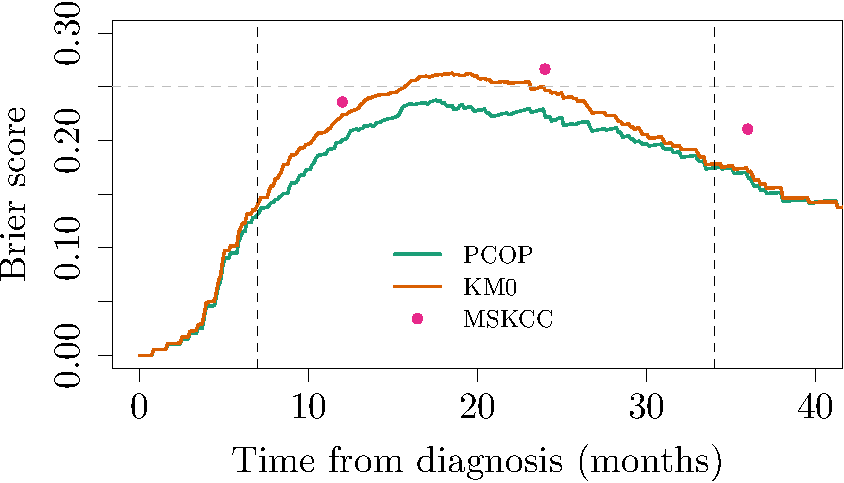
\includegraphics[width=\maxwidth]{figure/07-prob-bs-paths-plot-glasgow-1} 

}


\begin{kframe}\begin{alltt}
\hlkwd{plot}\hlstd{(gg.path.glasgow.brier}\hlopt{$}\hlstd{eval_times}\hlopt{/}\hlnum{365.25}\hlopt{*}\hlnum{12}\hlstd{, gg.path.glasgow.brier}\hlopt{$}\hlstd{bsc,} \hlkwc{col} \hlstd{= pal[}\hlstr{"gg"}\hlstd{],} \hlkwc{type} \hlstd{=} \hlstr{"l"}\hlstd{,} \hlkwc{ylim} \hlstd{=} \hlkwd{c}\hlstd{(}\hlnum{0}\hlstd{,} \hlnum{0.3}\hlstd{),} \hlkwc{xlab} \hlstd{=} \hlstr{"Time from diagnosis (months)"}\hlstd{,} \hlkwc{ylab} \hlstd{=} \hlstr{"Brier score"}\hlstd{,} \hlkwc{lwd} \hlstd{=} \hlnum{2}\hlstd{,} \hlkwc{xlim} \hlstd{=} \hlkwd{c}\hlstd{(}\hlnum{0}\hlstd{,} \hlnum{40}\hlstd{),} \hlkwc{main} \hlstd{=} \hlstr{"Glasgow"}\hlstd{)}
\hlkwd{lines}\hlstd{(gg.path.glasgow.brier}\hlopt{$}\hlstd{eval_times}\hlopt{/}\hlnum{365.25}\hlopt{*}\hlnum{12}\hlstd{, km0.path.glasgow.brier}\hlopt{$}\hlstd{bsc,} \hlkwc{col} \hlstd{= pal[}\hlstr{"km0"}\hlstd{],} \hlkwc{lwd} \hlstd{=} \hlnum{2}\hlstd{)}
\hlkwd{points}\hlstd{(}\hlkwd{c}\hlstd{(}\hlnum{12}\hlstd{,} \hlnum{24}\hlstd{,} \hlnum{36}\hlstd{),} \hlkwd{c}\hlstd{(mskcc_post.12mo.glasgow.brier, mskcc_post.24mo.glasgow.brier, mskcc_post.36mo.glasgow.brier),} \hlkwc{col} \hlstd{= pal[}\hlstr{"mskcc.pre"}\hlstd{],} \hlkwc{cex} \hlstd{=} \hlnum{1}\hlstd{,} \hlkwc{pch} \hlstd{=} \hlnum{16}\hlstd{)}
\hlkwd{points}\hlstd{(}\hlkwd{c}\hlstd{(}\hlnum{12}\hlstd{,} \hlnum{24}\hlstd{,} \hlnum{36}\hlstd{),} \hlkwd{c}\hlstd{(mskcc_pre.12mo.glasgow.brier, mskcc_pre.24mo.glasgow.brier, mskcc_pre.36mo.glasgow.brier),} \hlkwc{col} \hlstd{= pal[}\hlstr{"mskcc.post"}\hlstd{],} \hlkwc{cex} \hlstd{=} \hlnum{1}\hlstd{,} \hlkwc{pch} \hlstd{=} \hlnum{16}\hlstd{)}
\hlkwd{abline}\hlstd{(}\hlkwc{h} \hlstd{=} \hlnum{0.25}\hlstd{,} \hlkwc{col} \hlstd{=} \hlstr{"grey"}\hlstd{,} \hlkwc{lty} \hlstd{=} \hlstr{"dotted"}\hlstd{)}
\hlkwd{abline}\hlstd{(}\hlkwc{v} \hlstd{=} \hlkwd{c}\hlstd{(}\hlnum{7}\hlstd{,} \hlnum{34}\hlstd{))}
\hlkwd{legend}\hlstd{(}\hlstr{"bottom"}\hlstd{,}
        \hlkwc{legend} \hlstd{=} \hlkwd{c}\hlstd{(}     \hlstr{"GG1 Preop"}\hlstd{,}    \hlstr{"KM0"}\hlstd{,}          \hlstr{"MSKCC Postop"}\hlstd{,}         \hlstr{"MSKCC Preop"}\hlstd{),}
        \hlkwc{pch} \hlstd{=} \hlkwd{c}\hlstd{(}        \hlnum{NA}\hlstd{,}                     \hlnum{NA}\hlstd{,}             \hlnum{16}\hlstd{,}                             \hlnum{16}\hlstd{),}
        \hlkwc{col} \hlstd{=} \hlkwd{c}\hlstd{(        pal[}\hlstr{"gg"}\hlstd{],              pal[}\hlstr{"km0"}\hlstd{], pal[}\hlstr{"mskcc.pre"}\hlstd{],   pal[}\hlstr{"mskcc.post"}\hlstd{]),}
        \hlkwc{lty} \hlstd{=} \hlkwd{c}\hlstd{(}        \hlstr{"solid"}\hlstd{,}                \hlstr{"solid"}\hlstd{,}        \hlnum{NA}\hlstd{,}                             \hlnum{NA}\hlstd{),}
        \hlkwc{inset} \hlstd{=} \hlnum{0.05}\hlstd{,} \hlkwc{lwd} \hlstd{=} \hlnum{2}\hlstd{)}
\end{alltt}
\end{kframe}

{\centering 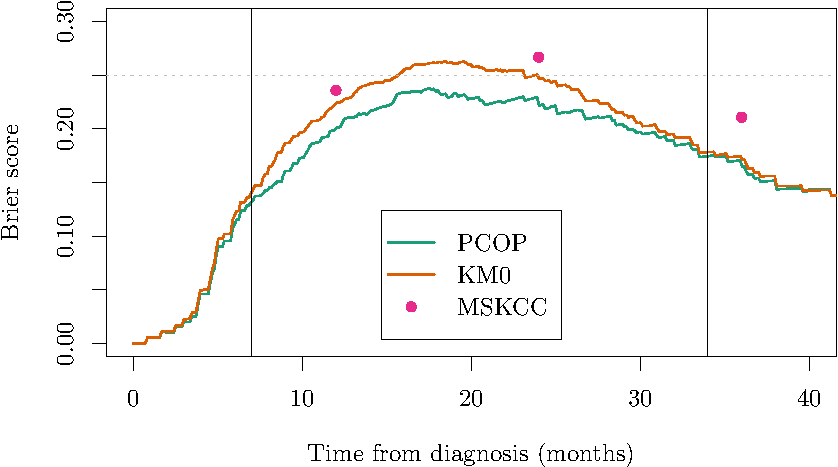
\includegraphics[width=\maxwidth]{figure/07-prob-bs-paths-plot-glasgow-2} 

}


\begin{kframe}\begin{alltt}
\hlkwd{plot}\hlstd{(gg.path.glasgow.brier}\hlopt{$}\hlstd{eval_times}\hlopt{/}\hlnum{365.25}\hlopt{*}\hlnum{12}\hlstd{, km0.path.glasgow.brier}\hlopt{$}\hlstd{bsc} \hlopt{-} \hlstd{gg.path.glasgow.brier}\hlopt{$}\hlstd{bsc,} \hlkwc{col} \hlstd{= pal[}\hlstr{"gg"}\hlstd{],} \hlkwc{type} \hlstd{=} \hlstr{"l"}\hlstd{,} \hlkwc{ylim} \hlstd{=} \hlkwd{c}\hlstd{(}\hlopt{-}\hlnum{0.05}\hlstd{,} \hlnum{0.05}\hlstd{),} \hlkwc{xlab} \hlstd{=} \hlstr{"Time from diagnosis (months)"}\hlstd{,} \hlkwc{ylab} \hlstd{=} \hlstr{"Brier score (Improvement over KM0)"}\hlstd{,} \hlkwc{lwd} \hlstd{=} \hlnum{2}\hlstd{,} \hlkwc{main} \hlstd{=} \hlstr{"Glasgow"}\hlstd{)}
\hlkwd{points}\hlstd{(}\hlkwd{c}\hlstd{(}\hlnum{12}\hlstd{,} \hlnum{24}\hlstd{,} \hlnum{36}\hlstd{),} \hlkwd{approx}\hlstd{(km0.path.glasgow.brier}\hlopt{$}\hlstd{eval_times}\hlopt{/}\hlnum{365.25}\hlopt{*}\hlnum{12}\hlstd{, km0.path.glasgow.brier}\hlopt{$}\hlstd{bsc,} \hlkwd{c}\hlstd{(}\hlnum{12}\hlstd{,} \hlnum{24}\hlstd{,} \hlnum{36}\hlstd{))}\hlopt{$}\hlstd{y} \hlopt{-} \hlkwd{c}\hlstd{(mskcc_post.12mo.glasgow.brier, mskcc_post.24mo.glasgow.brier, mskcc_post.36mo.glasgow.brier),} \hlkwc{col} \hlstd{= pal[}\hlstr{"mskcc.pre"}\hlstd{],} \hlkwc{cex} \hlstd{=} \hlnum{1}\hlstd{,} \hlkwc{pch} \hlstd{=} \hlnum{16}\hlstd{)}
\hlkwd{points}\hlstd{(}\hlkwd{c}\hlstd{(}\hlnum{12}\hlstd{,} \hlnum{24}\hlstd{,} \hlnum{36}\hlstd{),} \hlkwd{approx}\hlstd{(km0.path.glasgow.brier}\hlopt{$}\hlstd{eval_times}\hlopt{/}\hlnum{365.25}\hlopt{*}\hlnum{12}\hlstd{, km0.path.glasgow.brier}\hlopt{$}\hlstd{bsc,} \hlkwd{c}\hlstd{(}\hlnum{12}\hlstd{,} \hlnum{24}\hlstd{,} \hlnum{36}\hlstd{))}\hlopt{$}\hlstd{y} \hlopt{-} \hlkwd{c}\hlstd{(mskcc_pre.12mo.glasgow.brier, mskcc_pre.24mo.glasgow.brier, mskcc_pre.36mo.glasgow.brier),} \hlkwc{col} \hlstd{= pal[}\hlstr{"mskcc.post"}\hlstd{],} \hlkwc{cex} \hlstd{=} \hlnum{1}\hlstd{,} \hlkwc{pch} \hlstd{=} \hlnum{16}\hlstd{)}
\hlkwd{lines}\hlstd{(gg.path.glasgow.brier}\hlopt{$}\hlstd{eval_times}\hlopt{/}\hlnum{365.25}\hlopt{*}\hlnum{12}\hlstd{, km0.path.glasgow.brier}\hlopt{$}\hlstd{bsc} \hlopt{-} \hlnum{0.25}\hlstd{,} \hlkwc{col} \hlstd{=} \hlstr{"grey"}\hlstd{,} \hlkwc{lty} \hlstd{=} \hlstr{"dotted"}\hlstd{)}
\hlkwd{abline}\hlstd{(}\hlkwc{v} \hlstd{=} \hlkwd{c}\hlstd{(}\hlnum{7}\hlstd{,} \hlnum{34}\hlstd{))}
\hlkwd{abline}\hlstd{(}\hlkwc{h} \hlstd{=} \hlnum{0}\hlstd{,} \hlkwc{col} \hlstd{= pal[}\hlstr{"km0"}\hlstd{],} \hlkwc{lwd} \hlstd{=} \hlnum{2}\hlstd{)}
\hlkwd{legend}\hlstd{(}\hlstr{"topright"}\hlstd{,}
        \hlkwc{legend} \hlstd{=} \hlkwd{c}\hlstd{(}     \hlstr{"GG1 Preop"}\hlstd{,}    \hlstr{"MSKCC Postop"}\hlstd{,}         \hlstr{"MSKCC Preop"}\hlstd{),}
        \hlkwc{pch} \hlstd{=} \hlkwd{c}\hlstd{(}        \hlnum{NA}\hlstd{,}                     \hlnum{16}\hlstd{,}                             \hlnum{16}\hlstd{),}
        \hlkwc{col} \hlstd{=} \hlkwd{c}\hlstd{(        pal[}\hlstr{"gg"}\hlstd{],              pal[}\hlstr{"mskcc.pre"}\hlstd{],       pal[}\hlstr{"mskcc.post"}\hlstd{]),}
        \hlkwc{lty} \hlstd{=} \hlkwd{c}\hlstd{(}        \hlstr{"solid"}\hlstd{,}                \hlnum{NA}\hlstd{,}                             \hlnum{NA}\hlstd{),}
        \hlkwc{inset} \hlstd{=} \hlnum{0.05}\hlstd{,} \hlkwc{lwd} \hlstd{=} \hlnum{2}\hlstd{)}
\end{alltt}
\end{kframe}

{\centering 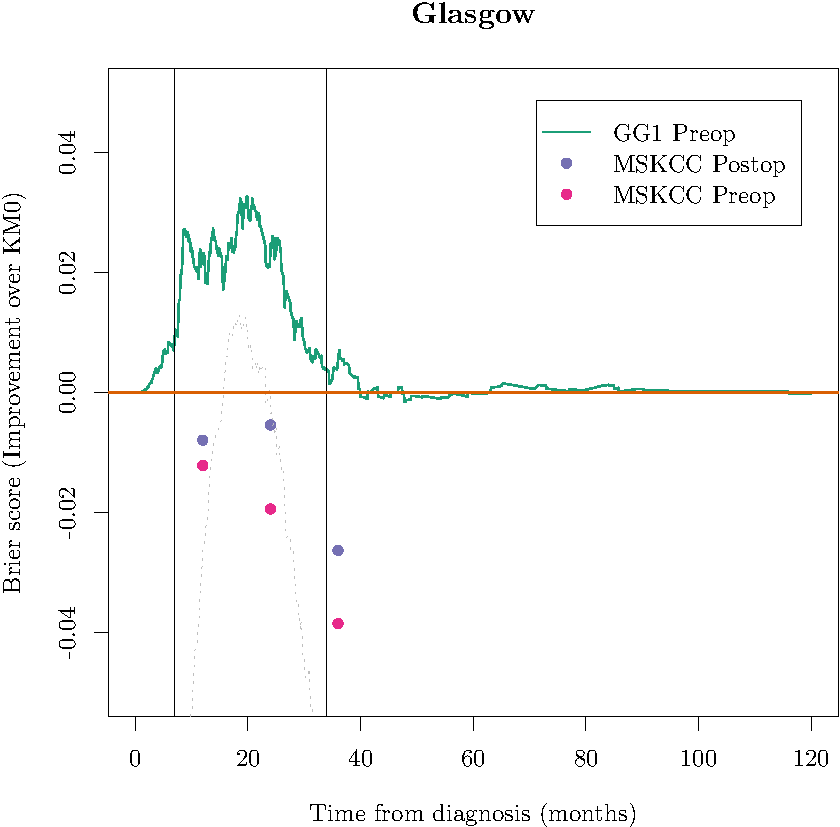
\includegraphics[width=\maxwidth]{figure/07-prob-bs-paths-plot-glasgow-3} 

}


\begin{kframe}\begin{alltt}
\hlkwd{plot}\hlstd{(gg.path.glasgow.brier}\hlopt{$}\hlstd{eval_times}\hlopt{/}\hlnum{365.25}\hlopt{*}\hlnum{12}\hlstd{, km0.path.glasgow.brier}\hlopt{$}\hlstd{bsc} \hlopt{-} \hlstd{gg.path.glasgow.brier}\hlopt{$}\hlstd{bsc,} \hlkwc{col} \hlstd{= pal[}\hlstr{"gg"}\hlstd{],} \hlkwc{type} \hlstd{=} \hlstr{"l"}\hlstd{,} \hlkwc{ylim} \hlstd{=} \hlkwd{c}\hlstd{(}\hlopt{-}\hlnum{0.05}\hlstd{,} \hlnum{0.05}\hlstd{),} \hlkwc{xlab} \hlstd{=} \hlstr{"Time from diagnosis (months)"}\hlstd{,} \hlkwc{ylab} \hlstd{=} \hlstr{"Brier score (Improvement over KM0)"}\hlstd{,} \hlkwc{lwd} \hlstd{=} \hlnum{2}\hlstd{,} \hlkwc{xlim} \hlstd{=} \hlkwd{c}\hlstd{(}\hlnum{0}\hlstd{,} \hlnum{40}\hlstd{),} \hlkwc{main} \hlstd{=} \hlstr{"Glasgow"}\hlstd{)}
\hlkwd{points}\hlstd{(}\hlkwd{c}\hlstd{(}\hlnum{12}\hlstd{,} \hlnum{24}\hlstd{,} \hlnum{36}\hlstd{),} \hlkwd{approx}\hlstd{(km0.path.glasgow.brier}\hlopt{$}\hlstd{eval_times}\hlopt{/}\hlnum{365.25}\hlopt{*}\hlnum{12}\hlstd{, km0.path.glasgow.brier}\hlopt{$}\hlstd{bsc,} \hlkwd{c}\hlstd{(}\hlnum{12}\hlstd{,} \hlnum{24}\hlstd{,} \hlnum{36}\hlstd{))}\hlopt{$}\hlstd{y} \hlopt{-} \hlkwd{c}\hlstd{(mskcc_post.12mo.glasgow.brier, mskcc_post.24mo.glasgow.brier, mskcc_post.36mo.glasgow.brier),} \hlkwc{col} \hlstd{= pal[}\hlstr{"mskcc.pre"}\hlstd{],} \hlkwc{cex} \hlstd{=} \hlnum{1}\hlstd{,} \hlkwc{pch} \hlstd{=} \hlnum{16}\hlstd{)}
\hlkwd{points}\hlstd{(}\hlkwd{c}\hlstd{(}\hlnum{12}\hlstd{,} \hlnum{24}\hlstd{,} \hlnum{36}\hlstd{),} \hlkwd{approx}\hlstd{(km0.path.glasgow.brier}\hlopt{$}\hlstd{eval_times}\hlopt{/}\hlnum{365.25}\hlopt{*}\hlnum{12}\hlstd{, km0.path.glasgow.brier}\hlopt{$}\hlstd{bsc,} \hlkwd{c}\hlstd{(}\hlnum{12}\hlstd{,} \hlnum{24}\hlstd{,} \hlnum{36}\hlstd{))}\hlopt{$}\hlstd{y} \hlopt{-} \hlkwd{c}\hlstd{(mskcc_pre.12mo.glasgow.brier, mskcc_pre.24mo.glasgow.brier, mskcc_pre.36mo.glasgow.brier),} \hlkwc{col} \hlstd{= pal[}\hlstr{"mskcc.post"}\hlstd{],} \hlkwc{cex} \hlstd{=} \hlnum{1}\hlstd{,} \hlkwc{pch} \hlstd{=} \hlnum{16}\hlstd{)}
\hlkwd{lines}\hlstd{(gg.path.glasgow.brier}\hlopt{$}\hlstd{eval_times}\hlopt{/}\hlnum{365.25}\hlopt{*}\hlnum{12}\hlstd{, km0.path.glasgow.brier}\hlopt{$}\hlstd{bsc} \hlopt{-} \hlnum{0.25}\hlstd{,} \hlkwc{col} \hlstd{=} \hlstr{"grey"}\hlstd{,} \hlkwc{lty} \hlstd{=} \hlstr{"dotted"}\hlstd{)}
\hlkwd{abline}\hlstd{(}\hlkwc{v} \hlstd{=} \hlkwd{c}\hlstd{(}\hlnum{7}\hlstd{,} \hlnum{34}\hlstd{))}
\hlkwd{abline}\hlstd{(}\hlkwc{h} \hlstd{=} \hlnum{0}\hlstd{,} \hlkwc{col} \hlstd{= pal[}\hlstr{"km0"}\hlstd{],} \hlkwc{lwd} \hlstd{=} \hlnum{2}\hlstd{)}
\hlkwd{legend}\hlstd{(}\hlstr{"bottom"}\hlstd{,}
        \hlkwc{legend} \hlstd{=} \hlkwd{c}\hlstd{(}     \hlstr{"GG1 Preop"}\hlstd{,}    \hlstr{"MSKCC Postop"}\hlstd{,}         \hlstr{"MSKCC Preop"}\hlstd{),}
        \hlkwc{pch} \hlstd{=} \hlkwd{c}\hlstd{(}        \hlnum{NA}\hlstd{,}                     \hlnum{16}\hlstd{,}                             \hlnum{16}\hlstd{),}
        \hlkwc{col} \hlstd{=} \hlkwd{c}\hlstd{(        pal[}\hlstr{"gg"}\hlstd{],              pal[}\hlstr{"mskcc.pre"}\hlstd{],       pal[}\hlstr{"mskcc.post"}\hlstd{]),}
        \hlkwc{lty} \hlstd{=} \hlkwd{c}\hlstd{(}        \hlstr{"solid"}\hlstd{,}                \hlnum{NA}\hlstd{,}                             \hlnum{NA}\hlstd{),}
        \hlkwc{inset} \hlstd{=} \hlnum{0.05}\hlstd{,} \hlkwc{lwd} \hlstd{=} \hlnum{2}\hlstd{)}
\end{alltt}
\end{kframe}

{\centering 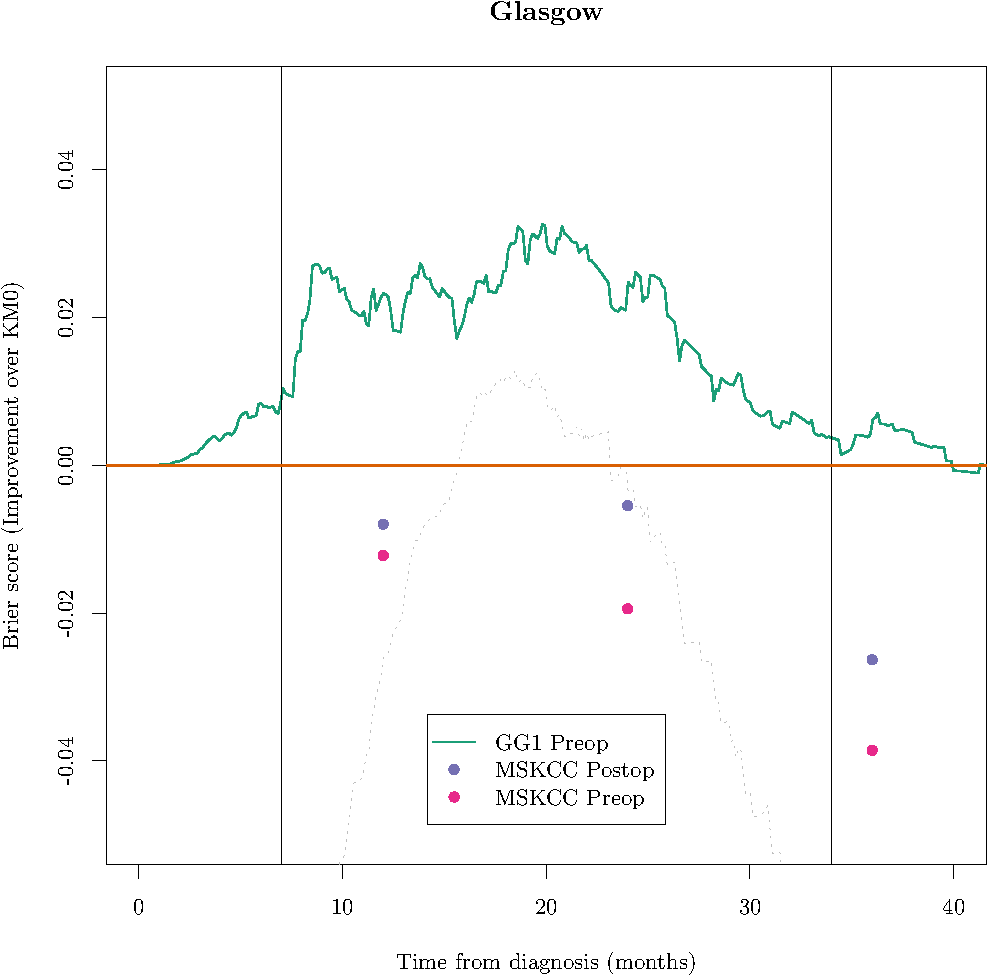
\includegraphics[width=\maxwidth]{figure/07-prob-bs-paths-plot-glasgow-4} 

}



\end{knitrout}


\begin{knitrout}
\definecolor{shadecolor}{rgb}{0.969, 0.969, 0.969}\color{fgcolor}\begin{kframe}
\begin{alltt}
\hlkwd{plot}\hlstd{(gg.path.apgi.brier}\hlopt{$}\hlstd{eval_times}\hlopt{/}\hlnum{365.25}\hlopt{*}\hlnum{12}\hlstd{, gg.path.apgi.brier}\hlopt{$}\hlstd{bsc,} \hlkwc{col} \hlstd{= pal[}\hlstr{"gg"}\hlstd{],} \hlkwc{type} \hlstd{=} \hlstr{"l"}\hlstd{,} \hlkwc{ylim} \hlstd{=} \hlkwd{c}\hlstd{(}\hlnum{0}\hlstd{,} \hlnum{0.3}\hlstd{),} \hlkwc{xlab} \hlstd{=} \hlstr{"Time from diagnosis (months)"}\hlstd{,} \hlkwc{ylab} \hlstd{=} \hlstr{"Brier score"}\hlstd{,} \hlkwc{lwd} \hlstd{=} \hlnum{2}\hlstd{,} \hlkwc{main} \hlstd{=} \hlstr{"APGI"}\hlstd{)}
\hlkwd{lines}\hlstd{(gg.path.apgi.brier}\hlopt{$}\hlstd{eval_times}\hlopt{/}\hlnum{365.25}\hlopt{*}\hlnum{12}\hlstd{, km0.path.apgi.brier}\hlopt{$}\hlstd{bsc,} \hlkwc{col} \hlstd{= pal[}\hlstr{"km0"}\hlstd{],} \hlkwc{lwd} \hlstd{=} \hlnum{2}\hlstd{)}
\hlkwd{points}\hlstd{(}\hlkwd{c}\hlstd{(}\hlnum{12}\hlstd{,} \hlnum{24}\hlstd{,} \hlnum{36}\hlstd{),} \hlkwd{c}\hlstd{(mskcc_post.12mo.apgi.brier, mskcc_post.24mo.apgi.brier, mskcc_post.36mo.apgi.brier),} \hlkwc{col} \hlstd{= pal[}\hlstr{"mskcc.pre"}\hlstd{],} \hlkwc{cex} \hlstd{=} \hlnum{1}\hlstd{,} \hlkwc{pch} \hlstd{=} \hlnum{16}\hlstd{)}
\hlkwd{points}\hlstd{(}\hlkwd{c}\hlstd{(}\hlnum{12}\hlstd{,} \hlnum{24}\hlstd{,} \hlnum{36}\hlstd{),} \hlkwd{c}\hlstd{(mskcc_pre.12mo.apgi.brier, mskcc_pre.24mo.apgi.brier, mskcc_pre.36mo.apgi.brier),} \hlkwc{col} \hlstd{= pal[}\hlstr{"mskcc.post"}\hlstd{],} \hlkwc{cex} \hlstd{=} \hlnum{1}\hlstd{,} \hlkwc{pch} \hlstd{=} \hlnum{16}\hlstd{)}
\hlkwd{abline}\hlstd{(}\hlkwc{h} \hlstd{=} \hlnum{0.25}\hlstd{,} \hlkwc{col} \hlstd{=} \hlstr{"grey"}\hlstd{,} \hlkwc{lty} \hlstd{=} \hlstr{"dotted"}\hlstd{)}
\hlkwd{abline}\hlstd{(}\hlkwc{v} \hlstd{=} \hlkwd{c}\hlstd{(}\hlnum{7}\hlstd{,} \hlnum{34}\hlstd{))}
\hlkwd{legend}\hlstd{(}\hlstr{"topright"}\hlstd{,}
        \hlkwc{legend} \hlstd{=} \hlkwd{c}\hlstd{(}     \hlstr{"GG1 Preop"}\hlstd{,}    \hlstr{"KM0"}\hlstd{,}          \hlstr{"MSKCC Postop"}\hlstd{,}         \hlstr{"MSKCC Preop"}\hlstd{),}
        \hlkwc{pch} \hlstd{=} \hlkwd{c}\hlstd{(}        \hlnum{NA}\hlstd{,}                     \hlnum{NA}\hlstd{,}             \hlnum{16}\hlstd{,}                             \hlnum{16}\hlstd{),}
        \hlkwc{col} \hlstd{=} \hlkwd{c}\hlstd{(        pal[}\hlstr{"gg"}\hlstd{],              pal[}\hlstr{"km0"}\hlstd{], pal[}\hlstr{"mskcc.pre"}\hlstd{],   pal[}\hlstr{"mskcc.post"}\hlstd{]),}
        \hlkwc{lty} \hlstd{=} \hlkwd{c}\hlstd{(}        \hlstr{"solid"}\hlstd{,}                \hlstr{"solid"}\hlstd{,}        \hlnum{NA}\hlstd{,}                             \hlnum{NA}\hlstd{),}
        \hlkwc{inset} \hlstd{=} \hlnum{0.05}\hlstd{,} \hlkwc{lwd} \hlstd{=} \hlnum{2}\hlstd{)}
\end{alltt}
\end{kframe}

{\centering 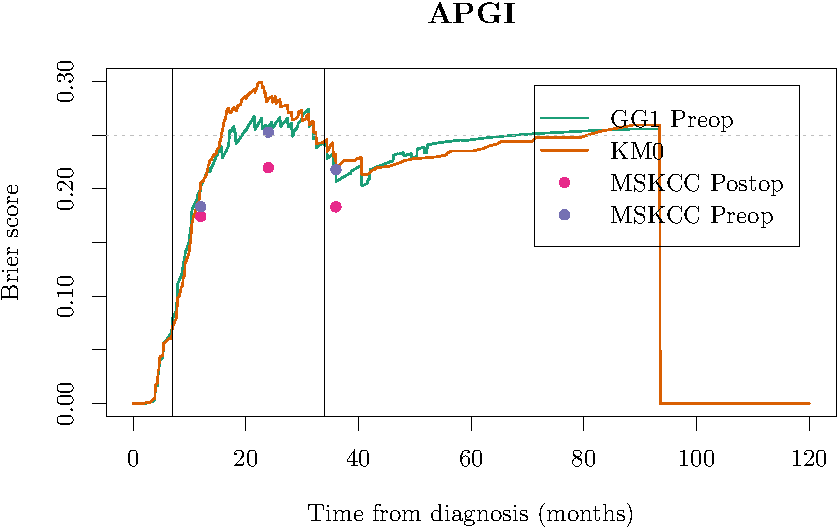
\includegraphics[width=\maxwidth]{figure/07-prob-bs-paths-plot-apgi-1} 

}


\begin{kframe}\begin{alltt}
\hlkwd{plot}\hlstd{(gg.path.apgi.brier}\hlopt{$}\hlstd{eval_times}\hlopt{/}\hlnum{365.25}\hlopt{*}\hlnum{12}\hlstd{, gg.path.apgi.brier}\hlopt{$}\hlstd{bsc,} \hlkwc{col} \hlstd{= pal[}\hlstr{"gg"}\hlstd{],} \hlkwc{type} \hlstd{=} \hlstr{"l"}\hlstd{,} \hlkwc{ylim} \hlstd{=} \hlkwd{c}\hlstd{(}\hlnum{0}\hlstd{,} \hlnum{0.3}\hlstd{),} \hlkwc{xlab} \hlstd{=} \hlstr{"Time from diagnosis (months)"}\hlstd{,} \hlkwc{ylab} \hlstd{=} \hlstr{"Brier score"}\hlstd{,} \hlkwc{lwd} \hlstd{=} \hlnum{2}\hlstd{,} \hlkwc{xlim} \hlstd{=} \hlkwd{c}\hlstd{(}\hlnum{0}\hlstd{,} \hlnum{40}\hlstd{),} \hlkwc{main} \hlstd{=} \hlstr{"APGI"}\hlstd{)}
\hlkwd{lines}\hlstd{(gg.path.apgi.brier}\hlopt{$}\hlstd{eval_times}\hlopt{/}\hlnum{365.25}\hlopt{*}\hlnum{12}\hlstd{, km0.path.apgi.brier}\hlopt{$}\hlstd{bsc,} \hlkwc{col} \hlstd{= pal[}\hlstr{"km0"}\hlstd{],} \hlkwc{lwd} \hlstd{=} \hlnum{2}\hlstd{)}
\hlkwd{points}\hlstd{(}\hlkwd{c}\hlstd{(}\hlnum{12}\hlstd{,} \hlnum{24}\hlstd{,} \hlnum{36}\hlstd{),} \hlkwd{c}\hlstd{(mskcc_post.12mo.apgi.brier, mskcc_post.24mo.apgi.brier, mskcc_post.36mo.apgi.brier),} \hlkwc{col} \hlstd{= pal[}\hlstr{"mskcc.pre"}\hlstd{],} \hlkwc{cex} \hlstd{=} \hlnum{1}\hlstd{,} \hlkwc{pch} \hlstd{=} \hlnum{16}\hlstd{)}
\hlkwd{points}\hlstd{(}\hlkwd{c}\hlstd{(}\hlnum{12}\hlstd{,} \hlnum{24}\hlstd{,} \hlnum{36}\hlstd{),} \hlkwd{c}\hlstd{(mskcc_pre.12mo.apgi.brier, mskcc_pre.24mo.apgi.brier, mskcc_pre.36mo.apgi.brier),} \hlkwc{col} \hlstd{= pal[}\hlstr{"mskcc.post"}\hlstd{],} \hlkwc{cex} \hlstd{=} \hlnum{1}\hlstd{,} \hlkwc{pch} \hlstd{=} \hlnum{16}\hlstd{)}
\hlkwd{abline}\hlstd{(}\hlkwc{h} \hlstd{=} \hlnum{0.25}\hlstd{,} \hlkwc{col} \hlstd{=} \hlstr{"grey"}\hlstd{,} \hlkwc{lty} \hlstd{=} \hlstr{"dotted"}\hlstd{)}
\hlkwd{abline}\hlstd{(}\hlkwc{v} \hlstd{=} \hlkwd{c}\hlstd{(}\hlnum{7}\hlstd{,} \hlnum{34}\hlstd{))}
\hlkwd{legend}\hlstd{(}\hlstr{"bottom"}\hlstd{,}
        \hlkwc{legend} \hlstd{=} \hlkwd{c}\hlstd{(}     \hlstr{"GG1 Preop"}\hlstd{,}    \hlstr{"KM0"}\hlstd{,}          \hlstr{"MSKCC Postop"}\hlstd{,}         \hlstr{"MSKCC Preop"}\hlstd{),}
        \hlkwc{pch} \hlstd{=} \hlkwd{c}\hlstd{(}        \hlnum{NA}\hlstd{,}                     \hlnum{NA}\hlstd{,}             \hlnum{16}\hlstd{,}                             \hlnum{16}\hlstd{),}
        \hlkwc{col} \hlstd{=} \hlkwd{c}\hlstd{(        pal[}\hlstr{"gg"}\hlstd{],              pal[}\hlstr{"km0"}\hlstd{], pal[}\hlstr{"mskcc.pre"}\hlstd{],   pal[}\hlstr{"mskcc.post"}\hlstd{]),}
        \hlkwc{lty} \hlstd{=} \hlkwd{c}\hlstd{(}        \hlstr{"solid"}\hlstd{,}                \hlstr{"solid"}\hlstd{,}        \hlnum{NA}\hlstd{,}                             \hlnum{NA}\hlstd{),}
        \hlkwc{inset} \hlstd{=} \hlnum{0.05}\hlstd{,} \hlkwc{lwd} \hlstd{=} \hlnum{2}\hlstd{)}
\end{alltt}
\end{kframe}

{\centering 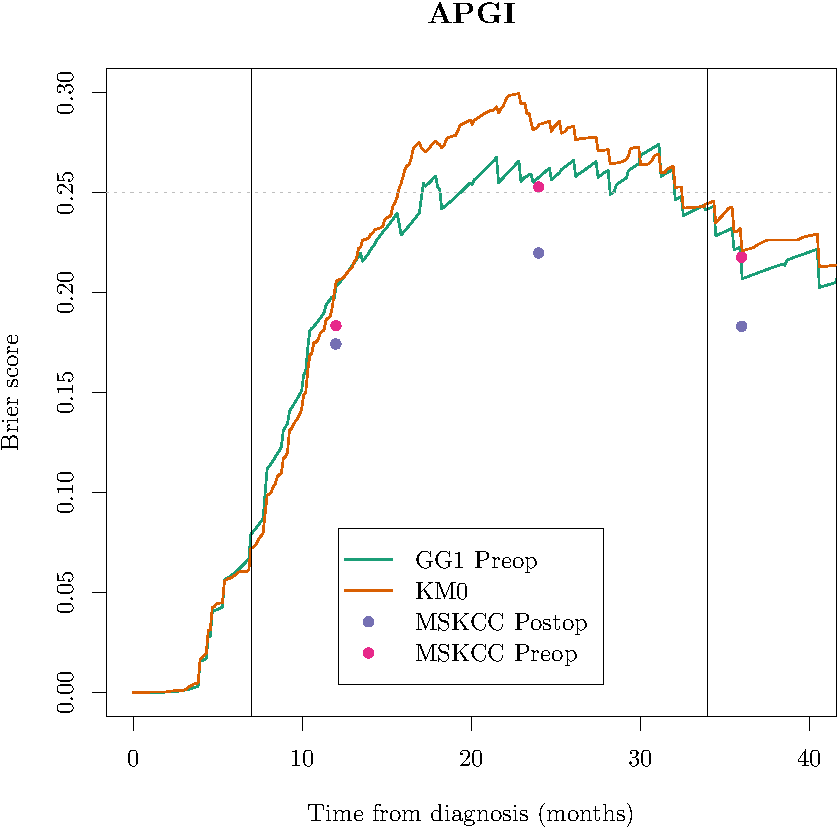
\includegraphics[width=\maxwidth]{figure/07-prob-bs-paths-plot-apgi-2} 

}


\begin{kframe}\begin{alltt}
\hlkwd{plot}\hlstd{(gg.path.apgi.brier}\hlopt{$}\hlstd{eval_times}\hlopt{/}\hlnum{365.25}\hlopt{*}\hlnum{12}\hlstd{, km0.path.apgi.brier}\hlopt{$}\hlstd{bsc} \hlopt{-} \hlstd{gg.path.apgi.brier}\hlopt{$}\hlstd{bsc,} \hlkwc{col} \hlstd{= pal[}\hlstr{"gg"}\hlstd{],} \hlkwc{type} \hlstd{=} \hlstr{"l"}\hlstd{,} \hlkwc{ylim} \hlstd{=} \hlkwd{c}\hlstd{(}\hlopt{-}\hlnum{0.05}\hlstd{,} \hlnum{0.05}\hlstd{),} \hlkwc{xlab} \hlstd{=} \hlstr{"Time from diagnosis (months)"}\hlstd{,} \hlkwc{ylab} \hlstd{=} \hlstr{"Brier score (Improvement over KM0)"}\hlstd{,} \hlkwc{lwd} \hlstd{=} \hlnum{2}\hlstd{,} \hlkwc{main} \hlstd{=} \hlstr{"APGI"}\hlstd{)}
\hlkwd{points}\hlstd{(}\hlkwd{c}\hlstd{(}\hlnum{12}\hlstd{,} \hlnum{24}\hlstd{,} \hlnum{36}\hlstd{),} \hlkwd{approx}\hlstd{(km0.path.apgi.brier}\hlopt{$}\hlstd{eval_times}\hlopt{/}\hlnum{365.25}\hlopt{*}\hlnum{12}\hlstd{, km0.path.apgi.brier}\hlopt{$}\hlstd{bsc,} \hlkwd{c}\hlstd{(}\hlnum{12}\hlstd{,} \hlnum{24}\hlstd{,} \hlnum{36}\hlstd{))}\hlopt{$}\hlstd{y} \hlopt{-} \hlkwd{c}\hlstd{(mskcc_post.12mo.apgi.brier, mskcc_post.24mo.apgi.brier, mskcc_post.36mo.apgi.brier),} \hlkwc{col} \hlstd{= pal[}\hlstr{"mskcc.pre"}\hlstd{],} \hlkwc{cex} \hlstd{=} \hlnum{1}\hlstd{,} \hlkwc{pch} \hlstd{=} \hlnum{16}\hlstd{)}
\hlkwd{points}\hlstd{(}\hlkwd{c}\hlstd{(}\hlnum{12}\hlstd{,} \hlnum{24}\hlstd{,} \hlnum{36}\hlstd{),} \hlkwd{approx}\hlstd{(km0.path.apgi.brier}\hlopt{$}\hlstd{eval_times}\hlopt{/}\hlnum{365.25}\hlopt{*}\hlnum{12}\hlstd{, km0.path.apgi.brier}\hlopt{$}\hlstd{bsc,} \hlkwd{c}\hlstd{(}\hlnum{12}\hlstd{,} \hlnum{24}\hlstd{,} \hlnum{36}\hlstd{))}\hlopt{$}\hlstd{y} \hlopt{-} \hlkwd{c}\hlstd{(mskcc_pre.12mo.apgi.brier, mskcc_pre.24mo.apgi.brier, mskcc_pre.36mo.apgi.brier),} \hlkwc{col} \hlstd{= pal[}\hlstr{"mskcc.post"}\hlstd{],} \hlkwc{cex} \hlstd{=} \hlnum{1}\hlstd{,} \hlkwc{pch} \hlstd{=} \hlnum{16}\hlstd{)}
\hlkwd{lines}\hlstd{(gg.path.apgi.brier}\hlopt{$}\hlstd{eval_times}\hlopt{/}\hlnum{365.25}\hlopt{*}\hlnum{12}\hlstd{, km0.path.apgi.brier}\hlopt{$}\hlstd{bsc} \hlopt{-} \hlnum{0.25}\hlstd{,} \hlkwc{col} \hlstd{=} \hlstr{"grey"}\hlstd{,} \hlkwc{lty} \hlstd{=} \hlstr{"dotted"}\hlstd{)}
\hlkwd{abline}\hlstd{(}\hlkwc{v} \hlstd{=} \hlkwd{c}\hlstd{(}\hlnum{7}\hlstd{,} \hlnum{34}\hlstd{))}
\hlkwd{abline}\hlstd{(}\hlkwc{h} \hlstd{=} \hlnum{0}\hlstd{,} \hlkwc{col} \hlstd{= pal[}\hlstr{"km0"}\hlstd{],} \hlkwc{lwd} \hlstd{=} \hlnum{2}\hlstd{)}
\hlkwd{legend}\hlstd{(}\hlstr{"topright"}\hlstd{,}
        \hlkwc{legend} \hlstd{=} \hlkwd{c}\hlstd{(}     \hlstr{"GG1 Preop"}\hlstd{,}    \hlstr{"MSKCC Postop"}\hlstd{,}         \hlstr{"MSKCC Preop"}\hlstd{),}
        \hlkwc{pch} \hlstd{=} \hlkwd{c}\hlstd{(}        \hlnum{NA}\hlstd{,}                     \hlnum{16}\hlstd{,}                             \hlnum{16}\hlstd{),}
        \hlkwc{col} \hlstd{=} \hlkwd{c}\hlstd{(        pal[}\hlstr{"gg"}\hlstd{],              pal[}\hlstr{"mskcc.pre"}\hlstd{],       pal[}\hlstr{"mskcc.post"}\hlstd{]),}
        \hlkwc{lty} \hlstd{=} \hlkwd{c}\hlstd{(}        \hlstr{"solid"}\hlstd{,}                \hlnum{NA}\hlstd{,}                             \hlnum{NA}\hlstd{),}
        \hlkwc{inset} \hlstd{=} \hlnum{0.05}\hlstd{,} \hlkwc{lwd} \hlstd{=} \hlnum{2}\hlstd{)}
\end{alltt}
\end{kframe}

{\centering 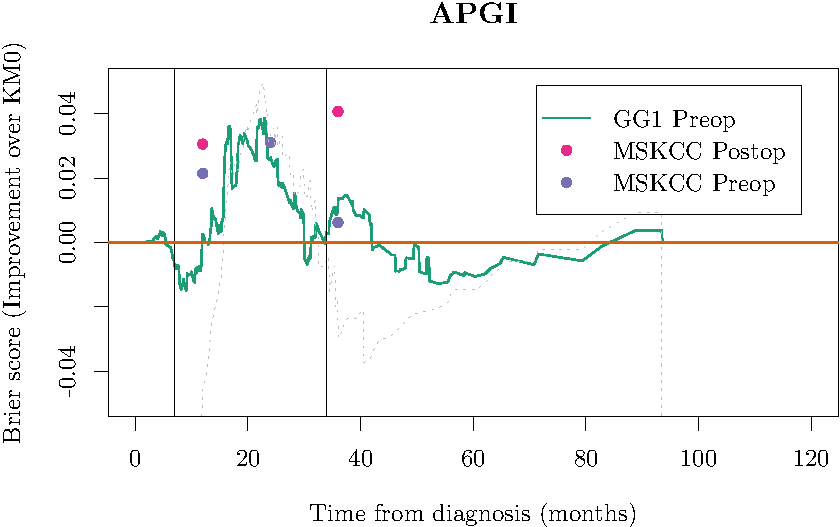
\includegraphics[width=\maxwidth]{figure/07-prob-bs-paths-plot-apgi-3} 

}


\begin{kframe}\begin{alltt}
\hlkwd{plot}\hlstd{(gg.path.apgi.brier}\hlopt{$}\hlstd{eval_times}\hlopt{/}\hlnum{365.25}\hlopt{*}\hlnum{12}\hlstd{, km0.path.apgi.brier}\hlopt{$}\hlstd{bsc} \hlopt{-} \hlstd{gg.path.apgi.brier}\hlopt{$}\hlstd{bsc,} \hlkwc{col} \hlstd{= pal[}\hlstr{"gg"}\hlstd{],} \hlkwc{type} \hlstd{=} \hlstr{"l"}\hlstd{,} \hlkwc{ylim} \hlstd{=} \hlkwd{c}\hlstd{(}\hlopt{-}\hlnum{0.05}\hlstd{,} \hlnum{0.05}\hlstd{),} \hlkwc{xlab} \hlstd{=} \hlstr{"Time from diagnosis (months)"}\hlstd{,} \hlkwc{ylab} \hlstd{=} \hlstr{"Brier score (Improvement over KM0)"}\hlstd{,} \hlkwc{lwd} \hlstd{=} \hlnum{2}\hlstd{,} \hlkwc{xlim} \hlstd{=} \hlkwd{c}\hlstd{(}\hlnum{0}\hlstd{,} \hlnum{40}\hlstd{),} \hlkwc{main} \hlstd{=} \hlstr{"APGI"}\hlstd{)}
\hlkwd{points}\hlstd{(}\hlkwd{c}\hlstd{(}\hlnum{12}\hlstd{,} \hlnum{24}\hlstd{,} \hlnum{36}\hlstd{),} \hlkwd{approx}\hlstd{(km0.path.apgi.brier}\hlopt{$}\hlstd{eval_times}\hlopt{/}\hlnum{365.25}\hlopt{*}\hlnum{12}\hlstd{, km0.path.apgi.brier}\hlopt{$}\hlstd{bsc,} \hlkwd{c}\hlstd{(}\hlnum{12}\hlstd{,} \hlnum{24}\hlstd{,} \hlnum{36}\hlstd{))}\hlopt{$}\hlstd{y} \hlopt{-} \hlkwd{c}\hlstd{(mskcc_post.12mo.apgi.brier, mskcc_post.24mo.apgi.brier, mskcc_post.36mo.apgi.brier),} \hlkwc{col} \hlstd{= pal[}\hlstr{"mskcc.pre"}\hlstd{],} \hlkwc{cex} \hlstd{=} \hlnum{1}\hlstd{,} \hlkwc{pch} \hlstd{=} \hlnum{16}\hlstd{)}
\hlkwd{points}\hlstd{(}\hlkwd{c}\hlstd{(}\hlnum{12}\hlstd{,} \hlnum{24}\hlstd{,} \hlnum{36}\hlstd{),} \hlkwd{approx}\hlstd{(km0.path.apgi.brier}\hlopt{$}\hlstd{eval_times}\hlopt{/}\hlnum{365.25}\hlopt{*}\hlnum{12}\hlstd{, km0.path.apgi.brier}\hlopt{$}\hlstd{bsc,} \hlkwd{c}\hlstd{(}\hlnum{12}\hlstd{,} \hlnum{24}\hlstd{,} \hlnum{36}\hlstd{))}\hlopt{$}\hlstd{y} \hlopt{-} \hlkwd{c}\hlstd{(mskcc_pre.12mo.apgi.brier, mskcc_pre.24mo.apgi.brier, mskcc_pre.36mo.apgi.brier),} \hlkwc{col} \hlstd{= pal[}\hlstr{"mskcc.post"}\hlstd{],} \hlkwc{cex} \hlstd{=} \hlnum{1}\hlstd{,} \hlkwc{pch} \hlstd{=} \hlnum{16}\hlstd{)}
\hlkwd{lines}\hlstd{(gg.path.apgi.brier}\hlopt{$}\hlstd{eval_times}\hlopt{/}\hlnum{365.25}\hlopt{*}\hlnum{12}\hlstd{, km0.path.apgi.brier}\hlopt{$}\hlstd{bsc} \hlopt{-} \hlnum{0.25}\hlstd{,} \hlkwc{col} \hlstd{=} \hlstr{"grey"}\hlstd{,} \hlkwc{lty} \hlstd{=} \hlstr{"dotted"}\hlstd{)}
\hlkwd{abline}\hlstd{(}\hlkwc{v} \hlstd{=} \hlkwd{c}\hlstd{(}\hlnum{7}\hlstd{,} \hlnum{34}\hlstd{))}
\hlkwd{abline}\hlstd{(}\hlkwc{h} \hlstd{=} \hlnum{0}\hlstd{,} \hlkwc{col} \hlstd{= pal[}\hlstr{"km0"}\hlstd{],} \hlkwc{lwd} \hlstd{=} \hlnum{2}\hlstd{)}
\hlkwd{legend}\hlstd{(}\hlstr{"bottom"}\hlstd{,}
        \hlkwc{legend} \hlstd{=} \hlkwd{c}\hlstd{(}     \hlstr{"GG1 Preop"}\hlstd{,}    \hlstr{"MSKCC Postop"}\hlstd{,}         \hlstr{"MSKCC Preop"}\hlstd{),}
        \hlkwc{pch} \hlstd{=} \hlkwd{c}\hlstd{(}        \hlnum{NA}\hlstd{,}                     \hlnum{16}\hlstd{,}                             \hlnum{16}\hlstd{),}
        \hlkwc{col} \hlstd{=} \hlkwd{c}\hlstd{(        pal[}\hlstr{"gg"}\hlstd{],              pal[}\hlstr{"mskcc.pre"}\hlstd{],       pal[}\hlstr{"mskcc.post"}\hlstd{]),}
        \hlkwc{lty} \hlstd{=} \hlkwd{c}\hlstd{(}        \hlstr{"solid"}\hlstd{,}                \hlnum{NA}\hlstd{,}                             \hlnum{NA}\hlstd{),}
        \hlkwc{inset} \hlstd{=} \hlnum{0.05}\hlstd{,} \hlkwc{lwd} \hlstd{=} \hlnum{2}\hlstd{)}
\end{alltt}
\end{kframe}

{\centering 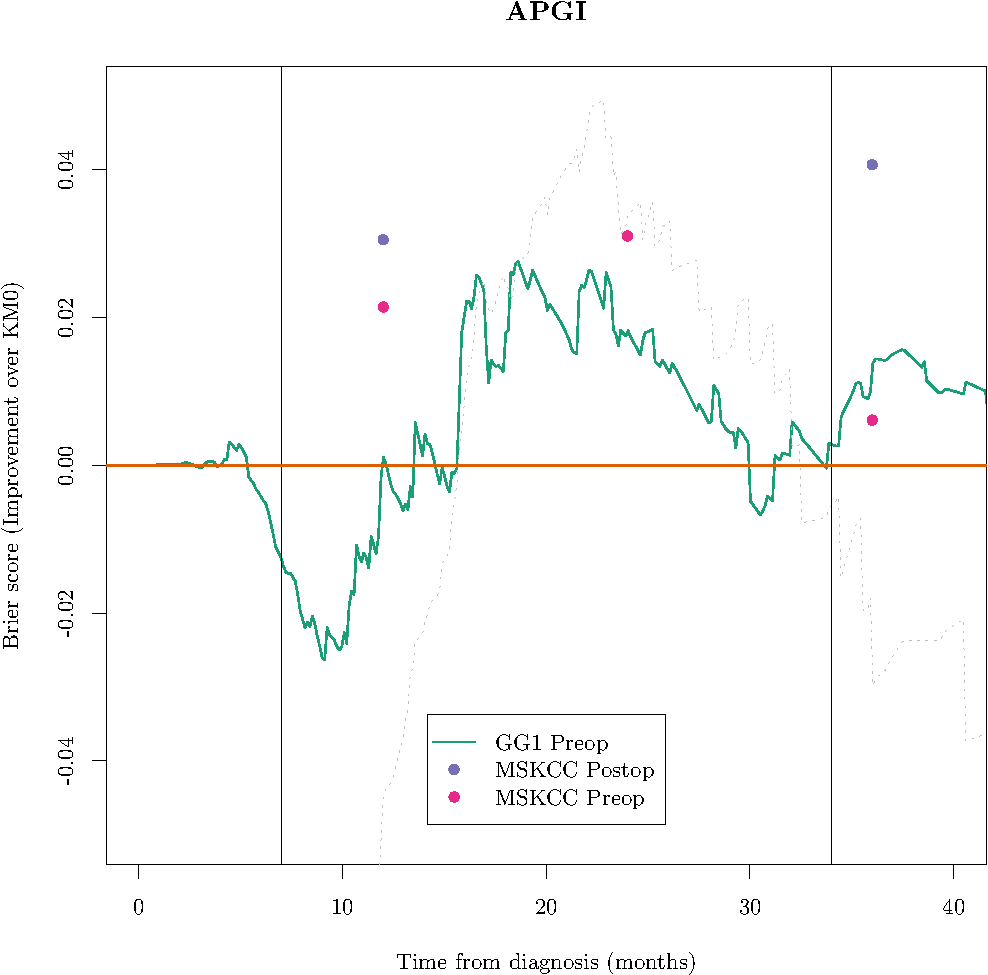
\includegraphics[width=\maxwidth]{figure/07-prob-bs-paths-plot-apgi-4} 

}



\end{knitrout}


\begin{knitrout}
\definecolor{shadecolor}{rgb}{0.969, 0.969, 0.969}\color{fgcolor}\begin{kframe}
\begin{alltt}
\hlstd{probs_bs_boot_func_glasgow} \hlkwb{=} \hlkwa{function}\hlstd{(}\hlkwc{d}\hlstd{,} \hlkwc{i}\hlstd{) \{}
        \hlstd{bs.mskcc.postop.12} \hlkwb{=} \hlkwd{calcBSsingle}\hlstd{(}\hlkwd{Surv}\hlstd{(d}\hlopt{$}\hlstd{Time[i], d}\hlopt{$}\hlstd{DSD[i]), mskcc_post.12mo.glasgow[i],} \hlnum{12}\hlopt{/}\hlnum{12}\hlopt{*}\hlnum{365.25}\hlstd{)}
        \hlstd{bs.mskcc.postop.24} \hlkwb{=} \hlkwd{calcBSsingle}\hlstd{(}\hlkwd{Surv}\hlstd{(d}\hlopt{$}\hlstd{Time[i], d}\hlopt{$}\hlstd{DSD[i]), mskcc_post.24mo.glasgow[i],} \hlnum{24}\hlopt{/}\hlnum{12}\hlopt{*}\hlnum{365.25}\hlstd{)}
        \hlstd{bs.mskcc.postop.36} \hlkwb{=} \hlkwd{calcBSsingle}\hlstd{(}\hlkwd{Surv}\hlstd{(d}\hlopt{$}\hlstd{Time[i], d}\hlopt{$}\hlstd{DSD[i]), mskcc_post.36mo.glasgow[i],} \hlnum{36}\hlopt{/}\hlnum{12}\hlopt{*}\hlnum{365.25}\hlstd{)}
        \hlstd{bs.mskcc.preop.12} \hlkwb{=} \hlkwd{calcBSsingle}\hlstd{(}\hlkwd{Surv}\hlstd{(d}\hlopt{$}\hlstd{Time[i], d}\hlopt{$}\hlstd{DSD[i]), mskcc_pre.12mo.glasgow[i],} \hlnum{12}\hlopt{/}\hlnum{12}\hlopt{*}\hlnum{365.25}\hlstd{)}
        \hlstd{bs.mskcc.preop.24} \hlkwb{=} \hlkwd{calcBSsingle}\hlstd{(}\hlkwd{Surv}\hlstd{(d}\hlopt{$}\hlstd{Time[i], d}\hlopt{$}\hlstd{DSD[i]), mskcc_pre.24mo.glasgow[i],} \hlnum{24}\hlopt{/}\hlnum{12}\hlopt{*}\hlnum{365.25}\hlstd{)}
        \hlstd{bs.mskcc.preop.36} \hlkwb{=} \hlkwd{calcBSsingle}\hlstd{(}\hlkwd{Surv}\hlstd{(d}\hlopt{$}\hlstd{Time[i], d}\hlopt{$}\hlstd{DSD[i]), mskcc_pre.36mo.glasgow[i],} \hlnum{36}\hlopt{/}\hlnum{12}\hlopt{*}\hlnum{365.25}\hlstd{)}

        \hlstd{bs.gg.vals} \hlkwb{=} \hlkwd{t}\hlstd{(}\hlkwd{sapply}\hlstd{(gg.path.glasgow[i],} \hlkwa{function}\hlstd{(}\hlkwc{path}\hlstd{)} \hlkwd{approx}\hlstd{(path[,}\hlnum{1}\hlstd{], path[,}\hlnum{2}\hlstd{],} \hlkwd{c}\hlstd{(}\hlnum{12}\hlstd{,} \hlnum{24}\hlstd{,} \hlnum{36}\hlstd{)}\hlopt{/}\hlnum{12}\hlopt{*}\hlnum{365.25}\hlstd{)}\hlopt{$}\hlstd{y))}
        \hlkwd{rownames}\hlstd{(bs.gg.vals)} \hlkwb{<-} \hlkwa{NULL}
        \hlstd{bs.gg.12} \hlkwb{=} \hlkwd{calcBSsingle}\hlstd{(}\hlkwd{Surv}\hlstd{(d}\hlopt{$}\hlstd{Time[i], d}\hlopt{$}\hlstd{DSD[i]), bs.gg.vals[,}\hlnum{1}\hlstd{],} \hlnum{12}\hlopt{/}\hlnum{12}\hlopt{*}\hlnum{365.25}\hlstd{)}
        \hlstd{bs.gg.24} \hlkwb{=} \hlkwd{calcBSsingle}\hlstd{(}\hlkwd{Surv}\hlstd{(d}\hlopt{$}\hlstd{Time[i], d}\hlopt{$}\hlstd{DSD[i]), bs.gg.vals[,}\hlnum{2}\hlstd{],} \hlnum{24}\hlopt{/}\hlnum{12}\hlopt{*}\hlnum{365.25}\hlstd{)}
        \hlstd{bs.gg.36} \hlkwb{=} \hlkwd{calcBSsingle}\hlstd{(}\hlkwd{Surv}\hlstd{(d}\hlopt{$}\hlstd{Time[i], d}\hlopt{$}\hlstd{DSD[i]), bs.gg.vals[,}\hlnum{3}\hlstd{],} \hlnum{36}\hlopt{/}\hlnum{12}\hlopt{*}\hlnum{365.25}\hlstd{)}

        \hlstd{bs.km0.vals} \hlkwb{=} \hlkwd{approx}\hlstd{(fit.km0}\hlopt{$}\hlstd{time, fit.km0}\hlopt{$}\hlstd{surv,} \hlkwd{c}\hlstd{(}\hlnum{12}\hlstd{,} \hlnum{24}\hlstd{,} \hlnum{36}\hlstd{)}\hlopt{/}\hlnum{12}\hlopt{*}\hlnum{365.25}\hlstd{)}\hlopt{$}\hlstd{y}
        \hlstd{bs.km0.12} \hlkwb{=} \hlkwd{calcBSsingle}\hlstd{(}\hlkwd{Surv}\hlstd{(d}\hlopt{$}\hlstd{Time[i], d}\hlopt{$}\hlstd{DSD[i]),} \hlkwd{rep}\hlstd{(bs.km0.vals[}\hlnum{1}\hlstd{],} \hlkwd{nrow}\hlstd{(d[i,])),} \hlnum{12}\hlopt{/}\hlnum{12}\hlopt{*}\hlnum{365.25}\hlstd{)}
        \hlstd{bs.km0.24} \hlkwb{=} \hlkwd{calcBSsingle}\hlstd{(}\hlkwd{Surv}\hlstd{(d}\hlopt{$}\hlstd{Time[i], d}\hlopt{$}\hlstd{DSD[i]),} \hlkwd{rep}\hlstd{(bs.km0.vals[}\hlnum{2}\hlstd{],} \hlkwd{nrow}\hlstd{(d[i,])),} \hlnum{24}\hlopt{/}\hlnum{12}\hlopt{*}\hlnum{365.25}\hlstd{)}
        \hlstd{bs.km0.36} \hlkwb{=} \hlkwd{calcBSsingle}\hlstd{(}\hlkwd{Surv}\hlstd{(d}\hlopt{$}\hlstd{Time[i], d}\hlopt{$}\hlstd{DSD[i]),} \hlkwd{rep}\hlstd{(bs.km0.vals[}\hlnum{3}\hlstd{],} \hlkwd{nrow}\hlstd{(d[i,])),} \hlnum{36}\hlopt{/}\hlnum{12}\hlopt{*}\hlnum{365.25}\hlstd{)}

        \hlstd{result} \hlkwb{=} \hlkwd{c}\hlstd{(}
                \hlstd{bs.gg.12} \hlopt{-} \hlstd{bs.km0.12,                   bs.mskcc.preop.12} \hlopt{-} \hlstd{bs.km0.12,}
                \hlstd{bs.gg.12} \hlopt{-} \hlstd{bs.mskcc.preop.12,}
                \hlstd{bs.gg.24} \hlopt{-} \hlstd{bs.km0.24,                   bs.mskcc.preop.24} \hlopt{-} \hlstd{bs.km0.24,}
                \hlstd{bs.gg.24} \hlopt{-} \hlstd{bs.mskcc.preop.24,}
                \hlstd{bs.gg.36} \hlopt{-} \hlstd{bs.km0.36,                   bs.mskcc.preop.36} \hlopt{-} \hlstd{bs.km0.36,}
                \hlstd{bs.gg.36} \hlopt{-} \hlstd{bs.mskcc.preop.36)}

        \hlkwd{names}\hlstd{(result)} \hlkwb{<-} \hlkwa{NULL}
        \hlstd{result}
\hlstd{\}}

\hlkwd{set.seed}\hlstd{(}\hlnum{20150208}\hlstd{)}
\hlstd{deltaBrier.boot.glasgow} \hlkwb{=} \hlkwd{boot}\hlstd{(data.glasgow, probs_bs_boot_func_glasgow,} \hlkwc{R} \hlstd{=} \hlnum{500}\hlstd{)}
\hlstd{deltaBrier.boot.glasgow.cis} \hlkwb{=} \hlkwd{t}\hlstd{(}\hlkwd{sapply}\hlstd{(}\hlnum{1}\hlopt{:}\hlkwd{ncol}\hlstd{(deltaBrier.boot.glasgow}\hlopt{$}\hlstd{t),} \hlkwa{function}\hlstd{(}\hlkwc{i}\hlstd{)} \hlkwd{boot.ci}\hlstd{(deltaBrier.boot.glasgow,} \hlkwc{index} \hlstd{= i,} \hlkwc{type} \hlstd{=} \hlstr{"bca"}\hlstd{)}\hlopt{$}\hlstd{bca))}
\hlkwd{colnames}\hlstd{(deltaBrier.boot.glasgow.cis)} \hlkwb{=} \hlkwd{c}\hlstd{(}\hlstr{"level"}\hlstd{,} \hlstr{"lowindex"}\hlstd{,} \hlstr{"highindex"}\hlstd{,} \hlstr{"lci"}\hlstd{,} \hlstr{"uci"}\hlstd{)}
\hlkwd{rownames}\hlstd{(deltaBrier.boot.glasgow.cis)} \hlkwb{=} \hlkwd{c}\hlstd{(}
        \hlstr{"12:gg-km0"}\hlstd{,} \hlstr{"12:pre-km0"}\hlstd{,} \hlstr{"12:gg-pre"}\hlstd{,}
        \hlstr{"24:gg-km0"}\hlstd{,} \hlstr{"24:pre-km0"}\hlstd{,} \hlstr{"24:gg-pre"}\hlstd{,}
        \hlstr{"36:gg-km0"}\hlstd{,} \hlstr{"36:pre-km0"}\hlstd{,} \hlstr{"36:gg-pre"}\hlstd{)}
\hlstd{deltaBrier.boot.glasgow}
\end{alltt}
\begin{verbatim}
## 
## ORDINARY NONPARAMETRIC BOOTSTRAP
## 
## 
## Call:
## boot(data = data.glasgow, statistic = probs_bs_boot_func_glasgow, 
##     R = 500)
## 
## 
## Bootstrap Statistics :
##      original     bias    std. error
## t1* -0.023252 -5.591e-04    0.011020
## t2*  0.012000  5.097e-04    0.014791
## t3* -0.035252 -1.069e-03    0.018703
## t4* -0.024707 -1.173e-03    0.011163
## t5*  0.020378  1.780e-04    0.020822
## t6* -0.045085 -1.351e-03    0.022651
## t7* -0.006137 -3.073e-04    0.006092
## t8*  0.039775 -9.123e-06    0.018277
## t9* -0.045912 -2.982e-04    0.018448
\end{verbatim}
\begin{alltt}
\hlstd{deltaBrier.boot.glasgow.cis}
\end{alltt}
\begin{verbatim}
##            level lowindex highindex        lci        uci
## 12:gg-km0   0.95    19.36     493.3 -0.0438016  0.0001641
## 12:pre-km0  0.95    10.07     485.4 -0.0179132  0.0401415
## 12:gg-pre   0.95     9.88     485.4 -0.0753277 -0.0035136
## 24:gg-km0   0.95    17.35     492.2 -0.0471870 -0.0023731
## 24:pre-km0  0.95    11.87     487.8 -0.0189747  0.0617515
## 24:gg-pre   0.95    19.24     493.3 -0.0845755  0.0024417
## 36:gg-km0   0.95    15.48     490.9 -0.0174246  0.0056702
## 36:pre-km0  0.95     7.75     482.0  0.0002576  0.0703455
## 36:gg-pre   0.95    17.88     492.7 -0.0791661 -0.0078058
\end{verbatim}
\end{kframe}
\end{knitrout}


\begin{knitrout}
\definecolor{shadecolor}{rgb}{0.969, 0.969, 0.969}\color{fgcolor}\begin{kframe}
\begin{alltt}
\hlstd{probs_bs_boot_func_apgi} \hlkwb{=} \hlkwa{function}\hlstd{(}\hlkwc{d}\hlstd{,} \hlkwc{i}\hlstd{) \{}
        \hlstd{bs.mskcc.postop.12} \hlkwb{=} \hlkwd{calcBSsingle}\hlstd{(}\hlkwd{Surv}\hlstd{(d}\hlopt{$}\hlstd{Time[i], d}\hlopt{$}\hlstd{DSD[i]), mskcc_post.12mo.apgi[i],} \hlnum{12}\hlopt{/}\hlnum{12}\hlopt{*}\hlnum{365.25}\hlstd{)}
        \hlstd{bs.mskcc.postop.24} \hlkwb{=} \hlkwd{calcBSsingle}\hlstd{(}\hlkwd{Surv}\hlstd{(d}\hlopt{$}\hlstd{Time[i], d}\hlopt{$}\hlstd{DSD[i]), mskcc_post.24mo.apgi[i],} \hlnum{24}\hlopt{/}\hlnum{12}\hlopt{*}\hlnum{365.25}\hlstd{)}
        \hlstd{bs.mskcc.postop.36} \hlkwb{=} \hlkwd{calcBSsingle}\hlstd{(}\hlkwd{Surv}\hlstd{(d}\hlopt{$}\hlstd{Time[i], d}\hlopt{$}\hlstd{DSD[i]), mskcc_post.36mo.apgi[i],} \hlnum{36}\hlopt{/}\hlnum{12}\hlopt{*}\hlnum{365.25}\hlstd{)}
        \hlstd{bs.mskcc.preop.12} \hlkwb{=} \hlkwd{calcBSsingle}\hlstd{(}\hlkwd{Surv}\hlstd{(d}\hlopt{$}\hlstd{Time[i], d}\hlopt{$}\hlstd{DSD[i]), mskcc_pre.12mo.apgi[i],} \hlnum{12}\hlopt{/}\hlnum{12}\hlopt{*}\hlnum{365.25}\hlstd{)}
        \hlstd{bs.mskcc.preop.24} \hlkwb{=} \hlkwd{calcBSsingle}\hlstd{(}\hlkwd{Surv}\hlstd{(d}\hlopt{$}\hlstd{Time[i], d}\hlopt{$}\hlstd{DSD[i]), mskcc_pre.24mo.apgi[i],} \hlnum{24}\hlopt{/}\hlnum{12}\hlopt{*}\hlnum{365.25}\hlstd{)}
        \hlstd{bs.mskcc.preop.36} \hlkwb{=} \hlkwd{calcBSsingle}\hlstd{(}\hlkwd{Surv}\hlstd{(d}\hlopt{$}\hlstd{Time[i], d}\hlopt{$}\hlstd{DSD[i]), mskcc_pre.36mo.apgi[i],} \hlnum{36}\hlopt{/}\hlnum{12}\hlopt{*}\hlnum{365.25}\hlstd{)}

        \hlstd{bs.gg.vals} \hlkwb{=} \hlkwd{t}\hlstd{(}\hlkwd{sapply}\hlstd{(gg.path.apgi[i],} \hlkwa{function}\hlstd{(}\hlkwc{path}\hlstd{)} \hlkwd{approx}\hlstd{(path[,}\hlnum{1}\hlstd{], path[,}\hlnum{2}\hlstd{],} \hlkwd{c}\hlstd{(}\hlnum{12}\hlstd{,} \hlnum{24}\hlstd{,} \hlnum{36}\hlstd{)}\hlopt{/}\hlnum{12}\hlopt{*}\hlnum{365.25}\hlstd{)}\hlopt{$}\hlstd{y))}
        \hlkwd{rownames}\hlstd{(bs.gg.vals)} \hlkwb{<-} \hlkwa{NULL}
        \hlstd{bs.gg.12} \hlkwb{=} \hlkwd{calcBSsingle}\hlstd{(}\hlkwd{Surv}\hlstd{(d}\hlopt{$}\hlstd{Time[i], d}\hlopt{$}\hlstd{DSD[i]), bs.gg.vals[,}\hlnum{1}\hlstd{],} \hlnum{12}\hlopt{/}\hlnum{12}\hlopt{*}\hlnum{365.25}\hlstd{)}
        \hlstd{bs.gg.24} \hlkwb{=} \hlkwd{calcBSsingle}\hlstd{(}\hlkwd{Surv}\hlstd{(d}\hlopt{$}\hlstd{Time[i], d}\hlopt{$}\hlstd{DSD[i]), bs.gg.vals[,}\hlnum{2}\hlstd{],} \hlnum{24}\hlopt{/}\hlnum{12}\hlopt{*}\hlnum{365.25}\hlstd{)}
        \hlstd{bs.gg.36} \hlkwb{=} \hlkwd{calcBSsingle}\hlstd{(}\hlkwd{Surv}\hlstd{(d}\hlopt{$}\hlstd{Time[i], d}\hlopt{$}\hlstd{DSD[i]), bs.gg.vals[,}\hlnum{3}\hlstd{],} \hlnum{36}\hlopt{/}\hlnum{12}\hlopt{*}\hlnum{365.25}\hlstd{)}

        \hlstd{bs.km0.vals} \hlkwb{=} \hlkwd{approx}\hlstd{(fit.km0}\hlopt{$}\hlstd{time, fit.km0}\hlopt{$}\hlstd{surv,} \hlkwd{c}\hlstd{(}\hlnum{12}\hlstd{,} \hlnum{24}\hlstd{,} \hlnum{36}\hlstd{)}\hlopt{/}\hlnum{12}\hlopt{*}\hlnum{365.25}\hlstd{)}\hlopt{$}\hlstd{y}
        \hlstd{bs.km0.12} \hlkwb{=} \hlkwd{calcBSsingle}\hlstd{(}\hlkwd{Surv}\hlstd{(d}\hlopt{$}\hlstd{Time[i], d}\hlopt{$}\hlstd{DSD[i]),} \hlkwd{rep}\hlstd{(bs.km0.vals[}\hlnum{1}\hlstd{],} \hlkwd{nrow}\hlstd{(d[i,])),} \hlnum{12}\hlopt{/}\hlnum{12}\hlopt{*}\hlnum{365.25}\hlstd{)}
        \hlstd{bs.km0.24} \hlkwb{=} \hlkwd{calcBSsingle}\hlstd{(}\hlkwd{Surv}\hlstd{(d}\hlopt{$}\hlstd{Time[i], d}\hlopt{$}\hlstd{DSD[i]),} \hlkwd{rep}\hlstd{(bs.km0.vals[}\hlnum{2}\hlstd{],} \hlkwd{nrow}\hlstd{(d[i,])),} \hlnum{24}\hlopt{/}\hlnum{12}\hlopt{*}\hlnum{365.25}\hlstd{)}
        \hlstd{bs.km0.36} \hlkwb{=} \hlkwd{calcBSsingle}\hlstd{(}\hlkwd{Surv}\hlstd{(d}\hlopt{$}\hlstd{Time[i], d}\hlopt{$}\hlstd{DSD[i]),} \hlkwd{rep}\hlstd{(bs.km0.vals[}\hlnum{3}\hlstd{],} \hlkwd{nrow}\hlstd{(d[i,])),} \hlnum{36}\hlopt{/}\hlnum{12}\hlopt{*}\hlnum{365.25}\hlstd{)}

        \hlstd{result} \hlkwb{=} \hlkwd{c}\hlstd{(}
                \hlstd{bs.gg.12} \hlopt{-} \hlstd{bs.km0.12,                   bs.mskcc.preop.12} \hlopt{-} \hlstd{bs.km0.12,}
                \hlstd{bs.gg.12} \hlopt{-} \hlstd{bs.mskcc.preop.12,}
                \hlstd{bs.gg.24} \hlopt{-} \hlstd{bs.km0.24,                   bs.mskcc.preop.24} \hlopt{-} \hlstd{bs.km0.24,}
                \hlstd{bs.gg.24} \hlopt{-} \hlstd{bs.mskcc.preop.24,}
                \hlstd{bs.gg.36} \hlopt{-} \hlstd{bs.km0.36,                   bs.mskcc.preop.36} \hlopt{-} \hlstd{bs.km0.36,}
                \hlstd{bs.gg.36} \hlopt{-} \hlstd{bs.mskcc.preop.36)}

        \hlkwd{names}\hlstd{(result)} \hlkwb{<-} \hlkwa{NULL}
        \hlstd{result}
\hlstd{\}}

\hlkwd{set.seed}\hlstd{(}\hlnum{20150208}\hlstd{)}
\hlstd{deltaBrier.boot.apgi} \hlkwb{=} \hlkwd{boot}\hlstd{(data.apgi, probs_bs_boot_func_apgi,} \hlkwc{R} \hlstd{=} \hlnum{500}\hlstd{)}
\hlstd{deltaBrier.boot.apgi.cis} \hlkwb{=} \hlkwd{t}\hlstd{(}\hlkwd{sapply}\hlstd{(}\hlnum{1}\hlopt{:}\hlkwd{ncol}\hlstd{(deltaBrier.boot.apgi}\hlopt{$}\hlstd{t),} \hlkwa{function}\hlstd{(}\hlkwc{i}\hlstd{)} \hlkwd{boot.ci}\hlstd{(deltaBrier.boot.apgi,} \hlkwc{index} \hlstd{= i,} \hlkwc{type} \hlstd{=} \hlstr{"bca"}\hlstd{)}\hlopt{$}\hlstd{bca))}
\hlkwd{colnames}\hlstd{(deltaBrier.boot.apgi.cis)} \hlkwb{=} \hlkwd{c}\hlstd{(}\hlstr{"level"}\hlstd{,} \hlstr{"lowindex"}\hlstd{,} \hlstr{"highindex"}\hlstd{,} \hlstr{"lci"}\hlstd{,} \hlstr{"uci"}\hlstd{)}
\hlkwd{rownames}\hlstd{(deltaBrier.boot.apgi.cis)} \hlkwb{=} \hlkwd{c}\hlstd{(}
        \hlstr{"12:gg-km0"}\hlstd{,} \hlstr{"12:pre-km0"}\hlstd{,} \hlstr{"12:gg-pre"}\hlstd{,}
        \hlstr{"24:gg-km0"}\hlstd{,} \hlstr{"24:pre-km0"}\hlstd{,} \hlstr{"24:gg-pre"}\hlstd{,}
        \hlstr{"36:gg-km0"}\hlstd{,} \hlstr{"36:pre-km0"}\hlstd{,} \hlstr{"36:gg-pre"}\hlstd{)}
\hlstd{deltaBrier.boot.apgi}
\end{alltt}
\begin{verbatim}
## 
## ORDINARY NONPARAMETRIC BOOTSTRAP
## 
## 
## Call:
## boot(data = data.apgi, statistic = probs_bs_boot_func_apgi, R = 500)
## 
## 
## Bootstrap Statistics :
##     original     bias    std. error
## t1* -0.00113 -0.0011691    0.015701
## t2* -0.02190 -0.0009299    0.018710
## t3*  0.02077 -0.0002392    0.028129
## t4* -0.01807  0.0005315    0.013458
## t5* -0.03102 -0.0029566    0.030885
## t6*  0.01295  0.0034881    0.034386
## t7* -0.01368  0.0004382    0.008461
## t8* -0.00230 -0.0019783    0.031044
## t9* -0.01138  0.0024165    0.031451
\end{verbatim}
\begin{alltt}
\hlstd{deltaBrier.boot.apgi.cis}
\end{alltt}
\begin{verbatim}
##            level lowindex highindex      lci      uci
## 12:gg-km0   0.95    14.99     490.7 -0.02914 0.029597
## 12:pre-km0  0.95    19.61     493.7 -0.05458 0.021352
## 12:gg-pre   0.95    11.55     487.5 -0.03594 0.073835
## 24:gg-km0   0.95    14.16     490.0 -0.04298 0.010080
## 24:pre-km0  0.95    24.25     495.0 -0.08215 0.036547
## 24:gg-pre   0.95     6.77     478.8 -0.06156 0.073555
## 36:gg-km0   0.95     6.89     480.5 -0.03200 0.001481
## 36:pre-km0  0.95    13.87     489.6 -0.06168 0.053566
## 36:gg-pre   0.95    15.08     490.8 -0.06278 0.051051
\end{verbatim}
\end{kframe}
\end{knitrout}


\begin{knitrout}
\definecolor{shadecolor}{rgb}{0.969, 0.969, 0.969}\color{fgcolor}\begin{kframe}
\begin{alltt}
\hlstd{temp.time} \hlkwb{=} \hlkwd{gsub}\hlstd{(}\hlstr{":.*"}\hlstd{,} \hlstr{""}\hlstd{,} \hlkwd{rownames}\hlstd{(deltaBrier.boot.glasgow.cis))}
\hlstd{temp.methodpos} \hlkwb{=} \hlkwd{gsub}\hlstd{(}\hlstr{".*:"}\hlstd{,} \hlstr{""}\hlstd{,} \hlkwd{gsub}\hlstd{(}\hlstr{"-.*"}\hlstd{,} \hlstr{""}\hlstd{,} \hlkwd{rownames}\hlstd{(deltaBrier.boot.glasgow.cis)))}
\hlstd{temp.methodneg} \hlkwb{=} \hlkwd{gsub}\hlstd{(}\hlstr{".*-"}\hlstd{,} \hlstr{""}\hlstd{,} \hlkwd{rownames}\hlstd{(deltaBrier.boot.glasgow.cis))}
\hlstd{temp.methods} \hlkwb{=} \hlkwd{sort}\hlstd{(}\hlkwd{unique}\hlstd{(}\hlkwd{c}\hlstd{(temp.methodpos, temp.methodneg)))}
\hlkwd{tapply}\hlstd{(}\hlnum{1}\hlopt{:}\hlkwd{length}\hlstd{(temp.time), temp.time,} \hlkwa{function}\hlstd{(}\hlkwc{is}\hlstd{) \{}
        \hlstd{res} \hlkwb{=} \hlkwd{matrix}\hlstd{(}\hlnum{0}\hlstd{,} \hlkwc{nrow} \hlstd{=} \hlkwd{length}\hlstd{(temp.methods),} \hlkwc{ncol} \hlstd{=} \hlkwd{length}\hlstd{(temp.methods))}
        \hlkwd{rownames}\hlstd{(res)} \hlkwb{=} \hlstd{temp.methods}
        \hlkwd{colnames}\hlstd{(res)} \hlkwb{=} \hlstd{temp.methods}
        \hlcom{# Make res signed.  0 => NS.  +1 => row is better than col (BS_row - BS_col < 0).  -1 => row is worse than col (BS_row - BS_col > 0).}
        \hlstd{res[}\hlkwd{cbind}\hlstd{(temp.methodpos[is], temp.methodneg[is])]} \hlkwb{=} \hlstd{(}\hlkwd{sign}\hlstd{(deltaBrier.boot.glasgow.cis[is,} \hlstr{"uci"}\hlstd{])} \hlopt{==} \hlkwd{sign}\hlstd{(deltaBrier.boot.glasgow.cis[is,} \hlstr{"lci"}\hlstd{]))} \hlopt{*} \hlkwd{sign}\hlstd{(}\hlopt{-}\hlstd{deltaBrier.boot.glasgow.cis[is,} \hlstr{"uci"}\hlstd{])}
        \hlstd{res[}\hlkwd{cbind}\hlstd{(temp.methodneg[is], temp.methodpos[is])]} \hlkwb{=} \hlstd{(}\hlkwd{sign}\hlstd{(deltaBrier.boot.glasgow.cis[is,} \hlstr{"uci"}\hlstd{])} \hlopt{==} \hlkwd{sign}\hlstd{(deltaBrier.boot.glasgow.cis[is,} \hlstr{"lci"}\hlstd{]))} \hlopt{*} \hlkwd{sign}\hlstd{(deltaBrier.boot.glasgow.cis[is,} \hlstr{"uci"}\hlstd{])}
        \hlstd{res}
\hlstd{\})}
\end{alltt}
\begin{verbatim}
## $`12`
##     gg km0 pre
## gg   0   0   1
## km0  0   0   0
## pre -1   0   0
## 
## $`24`
##     gg km0 pre
## gg   0   1   0
## km0 -1   0   0
## pre  0   0   0
## 
## $`36`
##     gg km0 pre
## gg   0   0   1
## km0  0   0   1
## pre -1  -1   0
\end{verbatim}
\end{kframe}
\end{knitrout}

\begin{knitrout}
\definecolor{shadecolor}{rgb}{0.969, 0.969, 0.969}\color{fgcolor}\begin{kframe}
\begin{alltt}
\hlstd{temp.time} \hlkwb{=} \hlkwd{gsub}\hlstd{(}\hlstr{":.*"}\hlstd{,} \hlstr{""}\hlstd{,} \hlkwd{rownames}\hlstd{(deltaBrier.boot.apgi.cis))}
\hlstd{temp.methodpos} \hlkwb{=} \hlkwd{gsub}\hlstd{(}\hlstr{".*:"}\hlstd{,} \hlstr{""}\hlstd{,} \hlkwd{gsub}\hlstd{(}\hlstr{"-.*"}\hlstd{,} \hlstr{""}\hlstd{,} \hlkwd{rownames}\hlstd{(deltaBrier.boot.apgi.cis)))}
\hlstd{temp.methodneg} \hlkwb{=} \hlkwd{gsub}\hlstd{(}\hlstr{".*-"}\hlstd{,} \hlstr{""}\hlstd{,} \hlkwd{rownames}\hlstd{(deltaBrier.boot.apgi.cis))}
\hlstd{temp.methods} \hlkwb{=} \hlkwd{sort}\hlstd{(}\hlkwd{unique}\hlstd{(}\hlkwd{c}\hlstd{(temp.methodpos, temp.methodneg)))}
\hlkwd{tapply}\hlstd{(}\hlnum{1}\hlopt{:}\hlkwd{length}\hlstd{(temp.time), temp.time,} \hlkwa{function}\hlstd{(}\hlkwc{is}\hlstd{) \{}
        \hlstd{res} \hlkwb{=} \hlkwd{matrix}\hlstd{(}\hlnum{0}\hlstd{,} \hlkwc{nrow} \hlstd{=} \hlkwd{length}\hlstd{(temp.methods),} \hlkwc{ncol} \hlstd{=} \hlkwd{length}\hlstd{(temp.methods))}
        \hlkwd{rownames}\hlstd{(res)} \hlkwb{=} \hlstd{temp.methods}
        \hlkwd{colnames}\hlstd{(res)} \hlkwb{=} \hlstd{temp.methods}
        \hlcom{# Make res signed.  0 => NS.  +1 => row is better than col (BS_row - BS_col < 0).  -1 => row is worse than col (BS_row - BS_col > 0).}
        \hlstd{res[}\hlkwd{cbind}\hlstd{(temp.methodpos[is], temp.methodneg[is])]} \hlkwb{=} \hlstd{(}\hlkwd{sign}\hlstd{(deltaBrier.boot.apgi.cis[is,} \hlstr{"uci"}\hlstd{])} \hlopt{==} \hlkwd{sign}\hlstd{(deltaBrier.boot.apgi.cis[is,} \hlstr{"lci"}\hlstd{]))} \hlopt{*} \hlkwd{sign}\hlstd{(}\hlopt{-}\hlstd{deltaBrier.boot.apgi.cis[is,} \hlstr{"uci"}\hlstd{])}
        \hlstd{res[}\hlkwd{cbind}\hlstd{(temp.methodneg[is], temp.methodpos[is])]} \hlkwb{=} \hlstd{(}\hlkwd{sign}\hlstd{(deltaBrier.boot.apgi.cis[is,} \hlstr{"uci"}\hlstd{])} \hlopt{==} \hlkwd{sign}\hlstd{(deltaBrier.boot.apgi.cis[is,} \hlstr{"lci"}\hlstd{]))} \hlopt{*} \hlkwd{sign}\hlstd{(deltaBrier.boot.apgi.cis[is,} \hlstr{"uci"}\hlstd{])}
        \hlstd{res}
\hlstd{\})}
\end{alltt}
\begin{verbatim}
## $`12`
##     gg km0 pre
## gg   0   0   0
## km0  0   0   0
## pre  0   0   0
## 
## $`24`
##     gg km0 pre
## gg   0   0   0
## km0  0   0   0
## pre  0   0   0
## 
## $`36`
##     gg km0 pre
## gg   0   0   0
## km0  0   0   0
## pre  0   0   0
\end{verbatim}
\end{kframe}
\end{knitrout}

Cumulative-dynamic:
\begin{knitrout}
\definecolor{shadecolor}{rgb}{0.969, 0.969, 0.969}\color{fgcolor}\begin{kframe}
\begin{alltt}
\hlstd{mskcc_pre.cdroc.glasgow} \hlkwb{=} \hlkwd{timeROC}\hlstd{(data.glasgow}\hlopt{$}\hlstd{Time}\hlopt{/}\hlnum{365.25}\hlopt{*}\hlnum{12}\hlstd{, data.glasgow}\hlopt{$}\hlstd{DSD, mskcc_pre.linpred.glasgow,} \hlkwc{cause} \hlstd{=} \hlnum{1}\hlstd{,} \hlkwc{times} \hlstd{=} \hlkwd{seq}\hlstd{(}\hlnum{1}\hlstd{,} \hlnum{36}\hlstd{,} \hlnum{1}\hlstd{),} \hlkwc{iid} \hlstd{=} \hlnum{TRUE}\hlstd{)}
\hlstd{mskcc_post.cdroc.glasgow} \hlkwb{=} \hlkwd{timeROC}\hlstd{(data.glasgow}\hlopt{$}\hlstd{Time}\hlopt{/}\hlnum{365.25}\hlopt{*}\hlnum{12}\hlstd{, data.glasgow}\hlopt{$}\hlstd{DSD, mskcc_post.linpred.glasgow,} \hlkwc{cause} \hlstd{=} \hlnum{1}\hlstd{,} \hlkwc{times} \hlstd{=} \hlkwd{seq}\hlstd{(}\hlnum{1}\hlstd{,} \hlnum{36}\hlstd{,} \hlnum{1}\hlstd{),} \hlkwc{iid} \hlstd{=} \hlnum{TRUE}\hlstd{)}
\hlstd{gg.cdroc.glasgow} \hlkwb{=} \hlkwd{timeROC}\hlstd{(data.glasgow}\hlopt{$}\hlstd{Time}\hlopt{/}\hlnum{365.25}\hlopt{*}\hlnum{12}\hlstd{, data.glasgow}\hlopt{$}\hlstd{DSD, gg.linpred.glasgow,} \hlkwc{cause} \hlstd{=} \hlnum{1}\hlstd{,} \hlkwc{times} \hlstd{=} \hlkwd{seq}\hlstd{(}\hlnum{1}\hlstd{,} \hlnum{36}\hlstd{,} \hlnum{1}\hlstd{),} \hlkwc{iid} \hlstd{=} \hlnum{TRUE}\hlstd{)}
\hlkwd{plotAUCcurve}\hlstd{(mskcc_pre.cdroc.glasgow,} \hlkwc{conf.int} \hlstd{=} \hlnum{FALSE}\hlstd{,} \hlkwc{add} \hlstd{=} \hlnum{FALSE}\hlstd{,} \hlkwc{col} \hlstd{= pal[}\hlstr{"mskcc.pre"}\hlstd{])}
\hlkwd{plotAUCcurve}\hlstd{(mskcc_post.cdroc.glasgow,} \hlkwc{conf.int} \hlstd{=} \hlnum{FALSE}\hlstd{,} \hlkwc{add} \hlstd{=} \hlnum{TRUE}\hlstd{,} \hlkwc{col} \hlstd{= pal[}\hlstr{"mskcc.post"}\hlstd{])}
\hlkwd{plotAUCcurve}\hlstd{(gg.cdroc.glasgow,} \hlkwc{conf.int} \hlstd{=} \hlnum{FALSE}\hlstd{,} \hlkwc{add} \hlstd{=} \hlnum{TRUE}\hlstd{,} \hlkwc{col} \hlstd{= pal[}\hlstr{"gg"}\hlstd{])}
\hlkwd{legend}\hlstd{(}\hlstr{"topright"}\hlstd{,} \hlkwc{legend} \hlstd{=} \hlkwd{c}\hlstd{(}\hlstr{"Glasgow Preop"}\hlstd{,} \hlstr{"Glasgow Postop"}\hlstd{,} \hlstr{"GG"}\hlstd{),} \hlkwc{col} \hlstd{=} \hlkwd{c}\hlstd{(pal[}\hlstr{"mskcc.pre"}\hlstd{], pal[}\hlstr{"mskcc.post"}\hlstd{], pal[}\hlstr{"gg"}\hlstd{]),} \hlkwc{lty} \hlstd{=} \hlstr{"solid"}\hlstd{,} \hlkwc{lwd} \hlstd{=} \hlnum{2}\hlstd{)}
\end{alltt}
\end{kframe}

{\centering 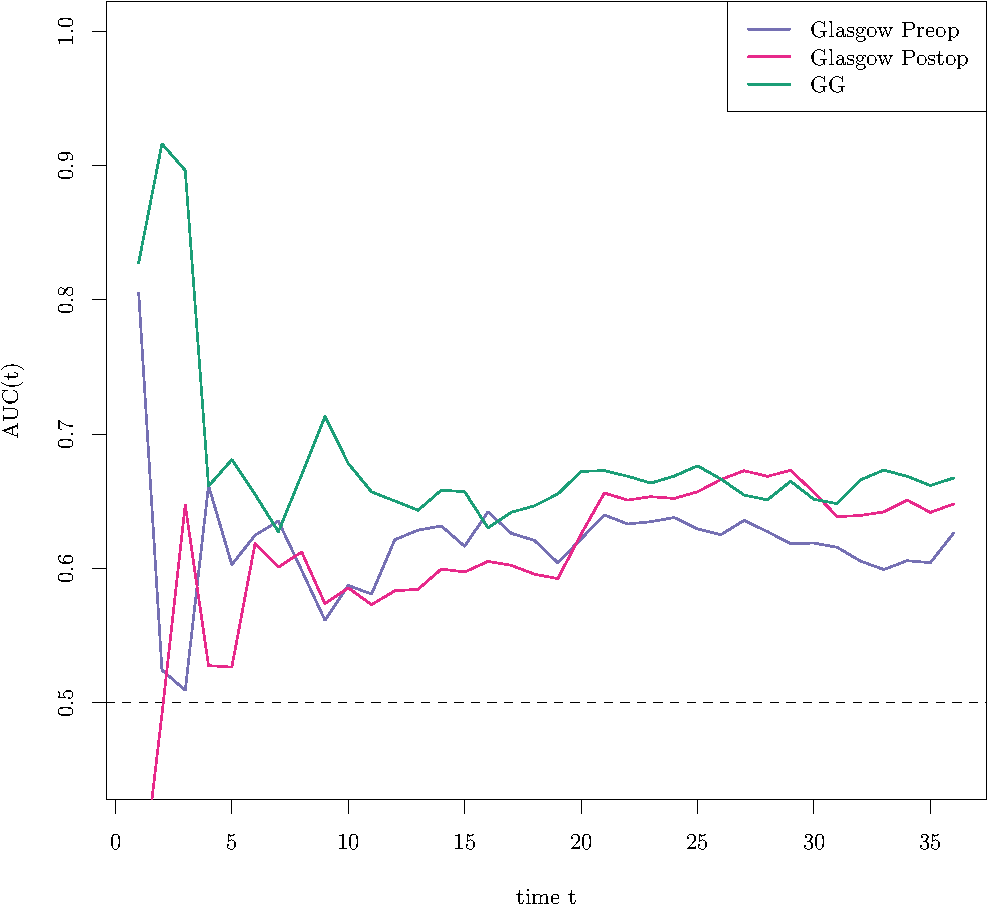
\includegraphics[width=\maxwidth]{figure/07-timeROC-glasgow-1} 

}



\end{knitrout}

\begin{knitrout}
\definecolor{shadecolor}{rgb}{0.969, 0.969, 0.969}\color{fgcolor}\begin{kframe}
\begin{alltt}
\hlstd{mskcc_pre.cdroc.apgi} \hlkwb{=} \hlkwd{timeROC}\hlstd{(data.apgi}\hlopt{$}\hlstd{Time}\hlopt{/}\hlnum{365.25}\hlopt{*}\hlnum{12}\hlstd{, data.apgi}\hlopt{$}\hlstd{DSD, mskcc_pre.linpred.apgi,} \hlkwc{cause} \hlstd{=} \hlnum{1}\hlstd{,} \hlkwc{times} \hlstd{=} \hlkwd{seq}\hlstd{(}\hlnum{1}\hlstd{,} \hlnum{36}\hlstd{,} \hlnum{1}\hlstd{),} \hlkwc{iid} \hlstd{=} \hlnum{TRUE}\hlstd{)}
\hlstd{mskcc_post.cdroc.apgi} \hlkwb{=} \hlkwd{timeROC}\hlstd{(data.apgi}\hlopt{$}\hlstd{Time}\hlopt{/}\hlnum{365.25}\hlopt{*}\hlnum{12}\hlstd{, data.apgi}\hlopt{$}\hlstd{DSD, mskcc_post.linpred.apgi,} \hlkwc{cause} \hlstd{=} \hlnum{1}\hlstd{,} \hlkwc{times} \hlstd{=} \hlkwd{seq}\hlstd{(}\hlnum{1}\hlstd{,} \hlnum{36}\hlstd{,} \hlnum{1}\hlstd{),} \hlkwc{iid} \hlstd{=} \hlnum{TRUE}\hlstd{)}
\hlstd{gg.cdroc.apgi} \hlkwb{=} \hlkwd{timeROC}\hlstd{(data.apgi}\hlopt{$}\hlstd{Time}\hlopt{/}\hlnum{365.25}\hlopt{*}\hlnum{12}\hlstd{, data.apgi}\hlopt{$}\hlstd{DSD, gg.linpred.apgi,} \hlkwc{cause} \hlstd{=} \hlnum{1}\hlstd{,} \hlkwc{times} \hlstd{=} \hlkwd{seq}\hlstd{(}\hlnum{1}\hlstd{,} \hlnum{36}\hlstd{,} \hlnum{1}\hlstd{),} \hlkwc{iid} \hlstd{=} \hlnum{TRUE}\hlstd{)}
\hlkwd{plotAUCcurve}\hlstd{(mskcc_pre.cdroc.apgi,} \hlkwc{conf.int} \hlstd{=} \hlnum{FALSE}\hlstd{,} \hlkwc{add} \hlstd{=} \hlnum{FALSE}\hlstd{,} \hlkwc{col} \hlstd{= pal[}\hlstr{"mskcc.pre"}\hlstd{])}
\hlkwd{plotAUCcurve}\hlstd{(mskcc_post.cdroc.apgi,} \hlkwc{conf.int} \hlstd{=} \hlnum{FALSE}\hlstd{,} \hlkwc{add} \hlstd{=} \hlnum{TRUE}\hlstd{,} \hlkwc{col} \hlstd{= pal[}\hlstr{"mskcc.post"}\hlstd{])}
\hlkwd{plotAUCcurve}\hlstd{(gg.cdroc.apgi,} \hlkwc{conf.int} \hlstd{=} \hlnum{FALSE}\hlstd{,} \hlkwc{add} \hlstd{=} \hlnum{TRUE}\hlstd{,} \hlkwc{col} \hlstd{= pal[}\hlstr{"gg"}\hlstd{])}
\hlkwd{legend}\hlstd{(}\hlstr{"topright"}\hlstd{,} \hlkwc{legend} \hlstd{=} \hlkwd{c}\hlstd{(}\hlstr{"APGI Preop"}\hlstd{,} \hlstr{"APGI Postop"}\hlstd{,} \hlstr{"GG"}\hlstd{),} \hlkwc{col} \hlstd{=} \hlkwd{c}\hlstd{(pal[}\hlstr{"mskcc.pre"}\hlstd{], pal[}\hlstr{"mskcc.post"}\hlstd{], pal[}\hlstr{"gg"}\hlstd{]),} \hlkwc{lty} \hlstd{=} \hlstr{"solid"}\hlstd{,} \hlkwc{lwd} \hlstd{=} \hlnum{2}\hlstd{)}
\hlkwd{abline}\hlstd{(}\hlkwc{v} \hlstd{=} \hlkwd{c}\hlstd{(}\hlnum{7}\hlstd{,} \hlnum{31}\hlstd{))}
\end{alltt}
\end{kframe}

{\centering 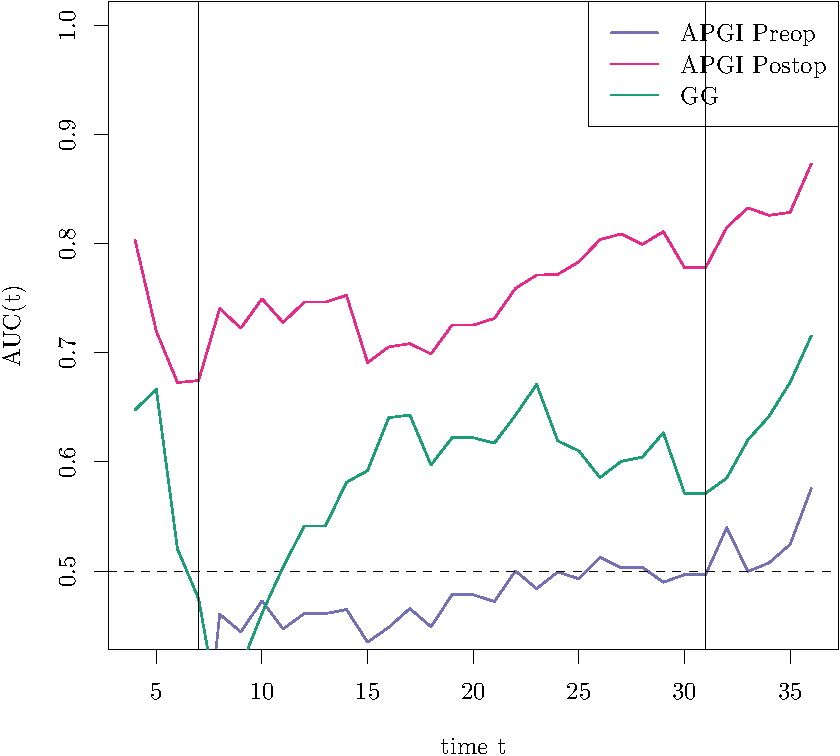
\includegraphics[width=\maxwidth]{figure/07-timeROC-apgi-1} 

}



\end{knitrout}

Incident-dynamic:
\begin{knitrout}
\definecolor{shadecolor}{rgb}{0.969, 0.969, 0.969}\color{fgcolor}\begin{kframe}
\begin{alltt}
\hlkwd{invisible}\hlstd{(}\hlkwd{risksetAUC}\hlstd{(data.glasgow}\hlopt{$}\hlstd{Time}\hlopt{/}\hlnum{365.25}\hlopt{*}\hlnum{12}\hlstd{,} \hlkwc{status} \hlstd{= data.glasgow}\hlopt{$}\hlstd{DSD,} \hlkwc{marker} \hlstd{= mskcc_pre.linpred.glasgow,} \hlkwc{tmax} \hlstd{=} \hlnum{36}\hlstd{,} \hlkwc{col} \hlstd{= pal[}\hlstr{"mskcc.pre"}\hlstd{],} \hlkwc{lwd} \hlstd{=} \hlnum{2}\hlstd{))}
\hlkwd{par}\hlstd{(}\hlkwc{new} \hlstd{=} \hlnum{TRUE}\hlstd{)}
\hlkwd{invisible}\hlstd{(}\hlkwd{risksetAUC}\hlstd{(data.glasgow}\hlopt{$}\hlstd{Time}\hlopt{/}\hlnum{365.25}\hlopt{*}\hlnum{12}\hlstd{,} \hlkwc{status} \hlstd{= data.glasgow}\hlopt{$}\hlstd{DSD,} \hlkwc{marker} \hlstd{= mskcc_post.linpred.glasgow,} \hlkwc{tmax} \hlstd{=} \hlnum{36}\hlstd{,} \hlkwc{col} \hlstd{= pal[}\hlstr{"mskcc.post"}\hlstd{],} \hlkwc{lwd} \hlstd{=} \hlnum{2}\hlstd{))}
\hlkwd{par}\hlstd{(}\hlkwc{new} \hlstd{=} \hlnum{TRUE}\hlstd{)}
\hlkwd{invisible}\hlstd{(}\hlkwd{risksetAUC}\hlstd{(data.glasgow}\hlopt{$}\hlstd{Time}\hlopt{/}\hlnum{365.25}\hlopt{*}\hlnum{12}\hlstd{,} \hlkwc{status} \hlstd{= data.glasgow}\hlopt{$}\hlstd{DSD,} \hlkwc{marker} \hlstd{= gg.linpred.glasgow,} \hlkwc{tmax} \hlstd{=} \hlnum{36}\hlstd{,} \hlkwc{col} \hlstd{= pal[}\hlstr{"gg"}\hlstd{],} \hlkwc{lwd} \hlstd{=} \hlnum{2}\hlstd{))}
\hlkwd{par}\hlstd{(}\hlkwc{new} \hlstd{=} \hlnum{TRUE}\hlstd{)}
\hlkwd{legend}\hlstd{(}\hlstr{"top"}\hlstd{,} \hlkwc{legend} \hlstd{=} \hlkwd{c}\hlstd{(}\hlstr{"Glasgow Preop"}\hlstd{,} \hlstr{"Glasgow Postop"}\hlstd{,} \hlstr{"GG"}\hlstd{),} \hlkwc{col} \hlstd{=} \hlkwd{c}\hlstd{(pal[}\hlstr{"mskcc.pre"}\hlstd{], pal[}\hlstr{"mskcc.post"}\hlstd{], pal[}\hlstr{"gg"}\hlstd{]),} \hlkwc{lty} \hlstd{=} \hlstr{"solid"}\hlstd{,} \hlkwc{lwd} \hlstd{=} \hlnum{2}\hlstd{)}
\hlkwd{abline}\hlstd{(}\hlkwc{v} \hlstd{=} \hlkwd{c}\hlstd{(}\hlnum{7}\hlstd{,} \hlnum{31}\hlstd{))}
\end{alltt}
\end{kframe}

{\centering 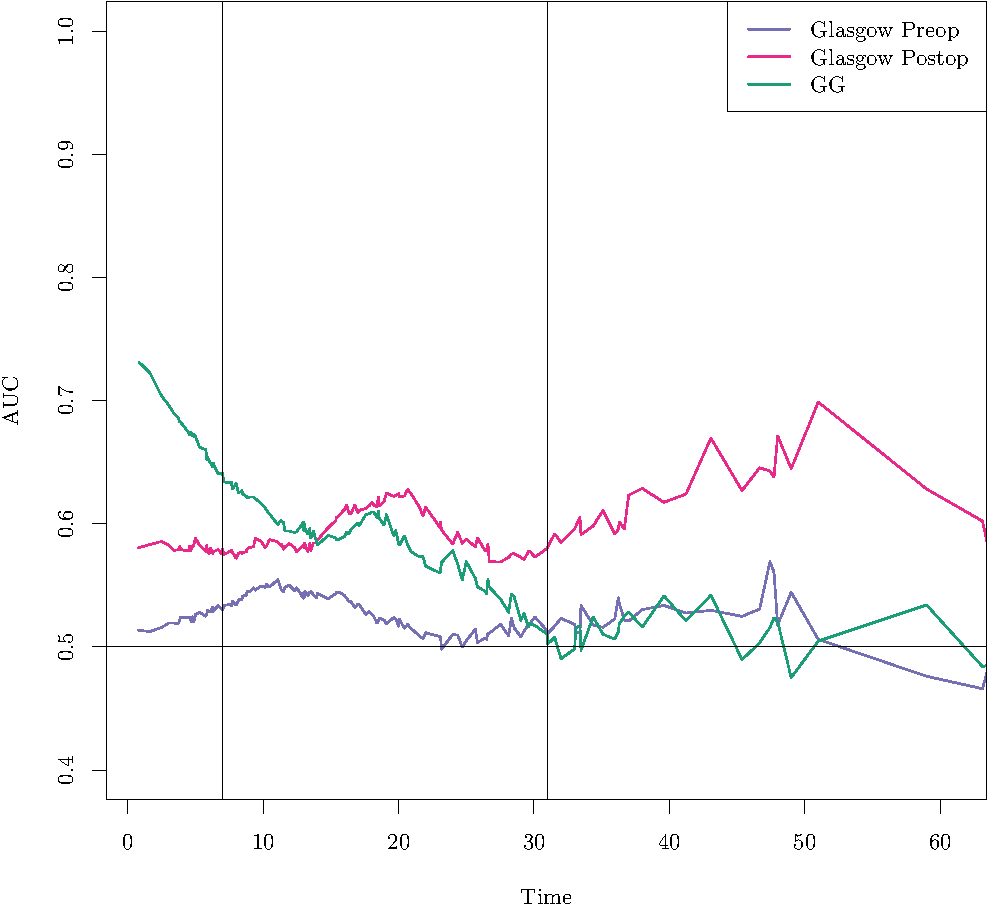
\includegraphics[width=\maxwidth]{figure/07-risksetROC-glasgow-1} 

}



\end{knitrout}

\begin{knitrout}
\definecolor{shadecolor}{rgb}{0.969, 0.969, 0.969}\color{fgcolor}\begin{kframe}
\begin{alltt}
\hlkwd{invisible}\hlstd{(}\hlkwd{risksetAUC}\hlstd{(data.apgi}\hlopt{$}\hlstd{Time}\hlopt{/}\hlnum{365.25}\hlopt{*}\hlnum{12}\hlstd{,} \hlkwc{status} \hlstd{= data.apgi}\hlopt{$}\hlstd{DSD,} \hlkwc{marker} \hlstd{= mskcc_pre.linpred.apgi,} \hlkwc{tmax} \hlstd{=} \hlnum{36}\hlstd{,} \hlkwc{col} \hlstd{= pal[}\hlstr{"mskcc.pre"}\hlstd{],} \hlkwc{lwd} \hlstd{=} \hlnum{2}\hlstd{))}
\hlkwd{par}\hlstd{(}\hlkwc{new} \hlstd{=} \hlnum{TRUE}\hlstd{)}
\hlkwd{invisible}\hlstd{(}\hlkwd{risksetAUC}\hlstd{(data.apgi}\hlopt{$}\hlstd{Time}\hlopt{/}\hlnum{365.25}\hlopt{*}\hlnum{12}\hlstd{,} \hlkwc{status} \hlstd{= data.apgi}\hlopt{$}\hlstd{DSD,} \hlkwc{marker} \hlstd{= mskcc_post.linpred.apgi,} \hlkwc{tmax} \hlstd{=} \hlnum{36}\hlstd{,} \hlkwc{col} \hlstd{= pal[}\hlstr{"mskcc.post"}\hlstd{],} \hlkwc{lwd} \hlstd{=} \hlnum{2}\hlstd{))}
\hlkwd{par}\hlstd{(}\hlkwc{new} \hlstd{=} \hlnum{TRUE}\hlstd{)}
\hlkwd{invisible}\hlstd{(}\hlkwd{risksetAUC}\hlstd{(data.apgi}\hlopt{$}\hlstd{Time}\hlopt{/}\hlnum{365.25}\hlopt{*}\hlnum{12}\hlstd{,} \hlkwc{status} \hlstd{= data.apgi}\hlopt{$}\hlstd{DSD,} \hlkwc{marker} \hlstd{= gg.linpred.apgi,} \hlkwc{tmax} \hlstd{=} \hlnum{36}\hlstd{,} \hlkwc{col} \hlstd{= pal[}\hlstr{"gg"}\hlstd{],} \hlkwc{lwd} \hlstd{=} \hlnum{2}\hlstd{))}
\hlkwd{par}\hlstd{(}\hlkwc{new} \hlstd{=} \hlnum{TRUE}\hlstd{)}
\hlkwd{legend}\hlstd{(}\hlstr{"top"}\hlstd{,} \hlkwc{legend} \hlstd{=} \hlkwd{c}\hlstd{(}\hlstr{"APGI Preop"}\hlstd{,} \hlstr{"APGI Postop"}\hlstd{,} \hlstr{"GG"}\hlstd{),} \hlkwc{col} \hlstd{=} \hlkwd{c}\hlstd{(pal[}\hlstr{"mskcc.pre"}\hlstd{], pal[}\hlstr{"mskcc.post"}\hlstd{], pal[}\hlstr{"gg"}\hlstd{]),} \hlkwc{lty} \hlstd{=} \hlstr{"solid"}\hlstd{,} \hlkwc{lwd} \hlstd{=} \hlnum{2}\hlstd{)}
\hlkwd{abline}\hlstd{(}\hlkwc{v} \hlstd{=} \hlkwd{c}\hlstd{(}\hlnum{7}\hlstd{,} \hlnum{31}\hlstd{))}
\end{alltt}
\end{kframe}

{\centering 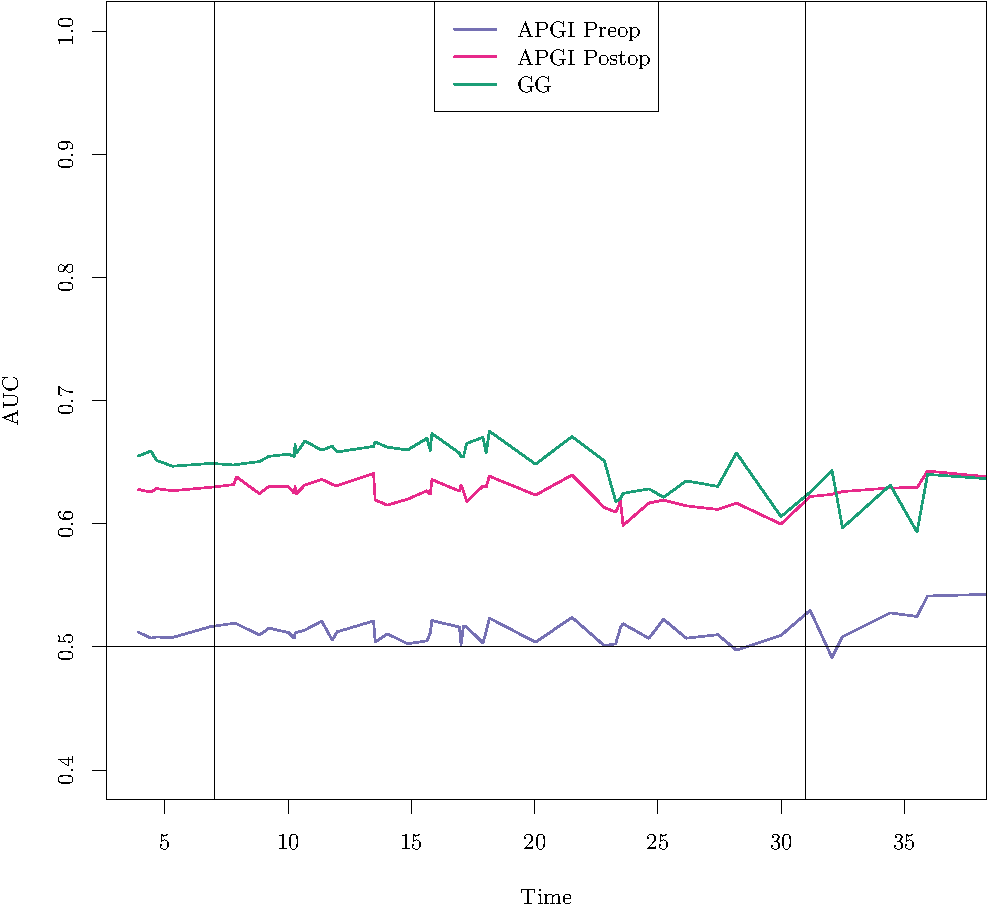
\includegraphics[width=\maxwidth]{figure/07-risksetROC-apgi-1} 

}



\end{knitrout}

\end{document}
